% !Mode:: "TeX:UTF-8"
%!TEX program  = xelatex
%中国光谷·“华为杯”第十九届中国研究生数学建模竞赛论文格式规范:
%论文题目和摘要写在论文摘要上,摘要页的下一页开始论文正文;
%论文从摘要页开始编写页码,页码必须位于每页页脚中部,用阿拉伯数字从“1 ”开始连续编号;
%论文题目用三号黑体字、一级标题用四号黑体字,并居中;
%论文中其他汉字一律采用小四号宋体字,行距用单倍行距。计算机结果和源程序需在规定时间内上传竞赛系统以备检查。
%请大家注意:摘要应该是一份简明扼要的详细摘要(包括关键词),请认真书写(注意篇幅一般不超过两页,且无需译成英文)。全国评阅时对摘要和论文都会审阅。
%论文不能有页眉,论文中不能有任何可能显示答题人身份的标志。

\documentclass[a4paper]{CPIPC}
\usepackage{xeCJK}
\usepackage{ctex}
\usepackage[top=30.0mm,bottom=25.0mm,left=22.5mm,right=22.5mm,headsep=8mm]{geometry}%设置页边距
\usepackage{array} %主要是增加列样式选项
\usepackage[dvipsnames]{xcolor}%颜色宏包
\usepackage{graphicx}%图片宏包
\usepackage{amsmath}%公式宏包
\usepackage{amssymb}
\usepackage{float} %限制浮动体的位置
\usepackage{pdfpages}
\usepackage{listings}
\usepackage{titletoc}
\usepackage{shadowtext}%大赛标题加阴影
\usepackage{booktabs}
\usepackage{subfigure}
\usepackage{subcaption}
\usepackage{algorithm}
\usepackage{algorithmic}

\usepackage{enumerate}
\usepackage{xcolor}
\usepackage{colortbl}
\usepackage{booktabs} % For improved table lines
\definecolor{color3}{RGB}{255, 255, 200}
\definecolor{color2}{RGB}{255, 220, 200}
\definecolor{color1}{RGB}{255, 181, 163}
\newcommand{\cc}[1]{\cellcolor{color#1}}

\renewcommand{\baselinestretch}{1.4} %设置单倍行距
  
\numberwithin{equation}{section}
% \usepackage{newtxtext, newtxmath}  %使用Times Nxew Roman 字体的方法

\lstset{
    language = Python,
    backgroundcolor = \color{white!10},    % 背景色:淡黄
    basicstyle = \small\ttfamily,           % 基本样式 + 小号字体
    rulesepcolor= \color{gray},             % 代码块边框颜色
    breaklines = true,                  % 代码过长则换行
    %numbers = left,                     % 行号在左侧显示
    %numberstyle = \small,               % 行号字体
    keywordstyle = \color{black},            % 关键字颜色
    commentstyle =\color{green!100},        % 注释颜色
    stringstyle = \color{red!100},          % 字符串颜色
    frame =  tb,                  % 用(带影子效果)方框框住代码块
    showspaces = false,                 % 不显示空格
    columns = fixed,                    % 字间距固定
}

%--------------------正文----------------------
\begin{document}


\numberwithin{equation}{section}
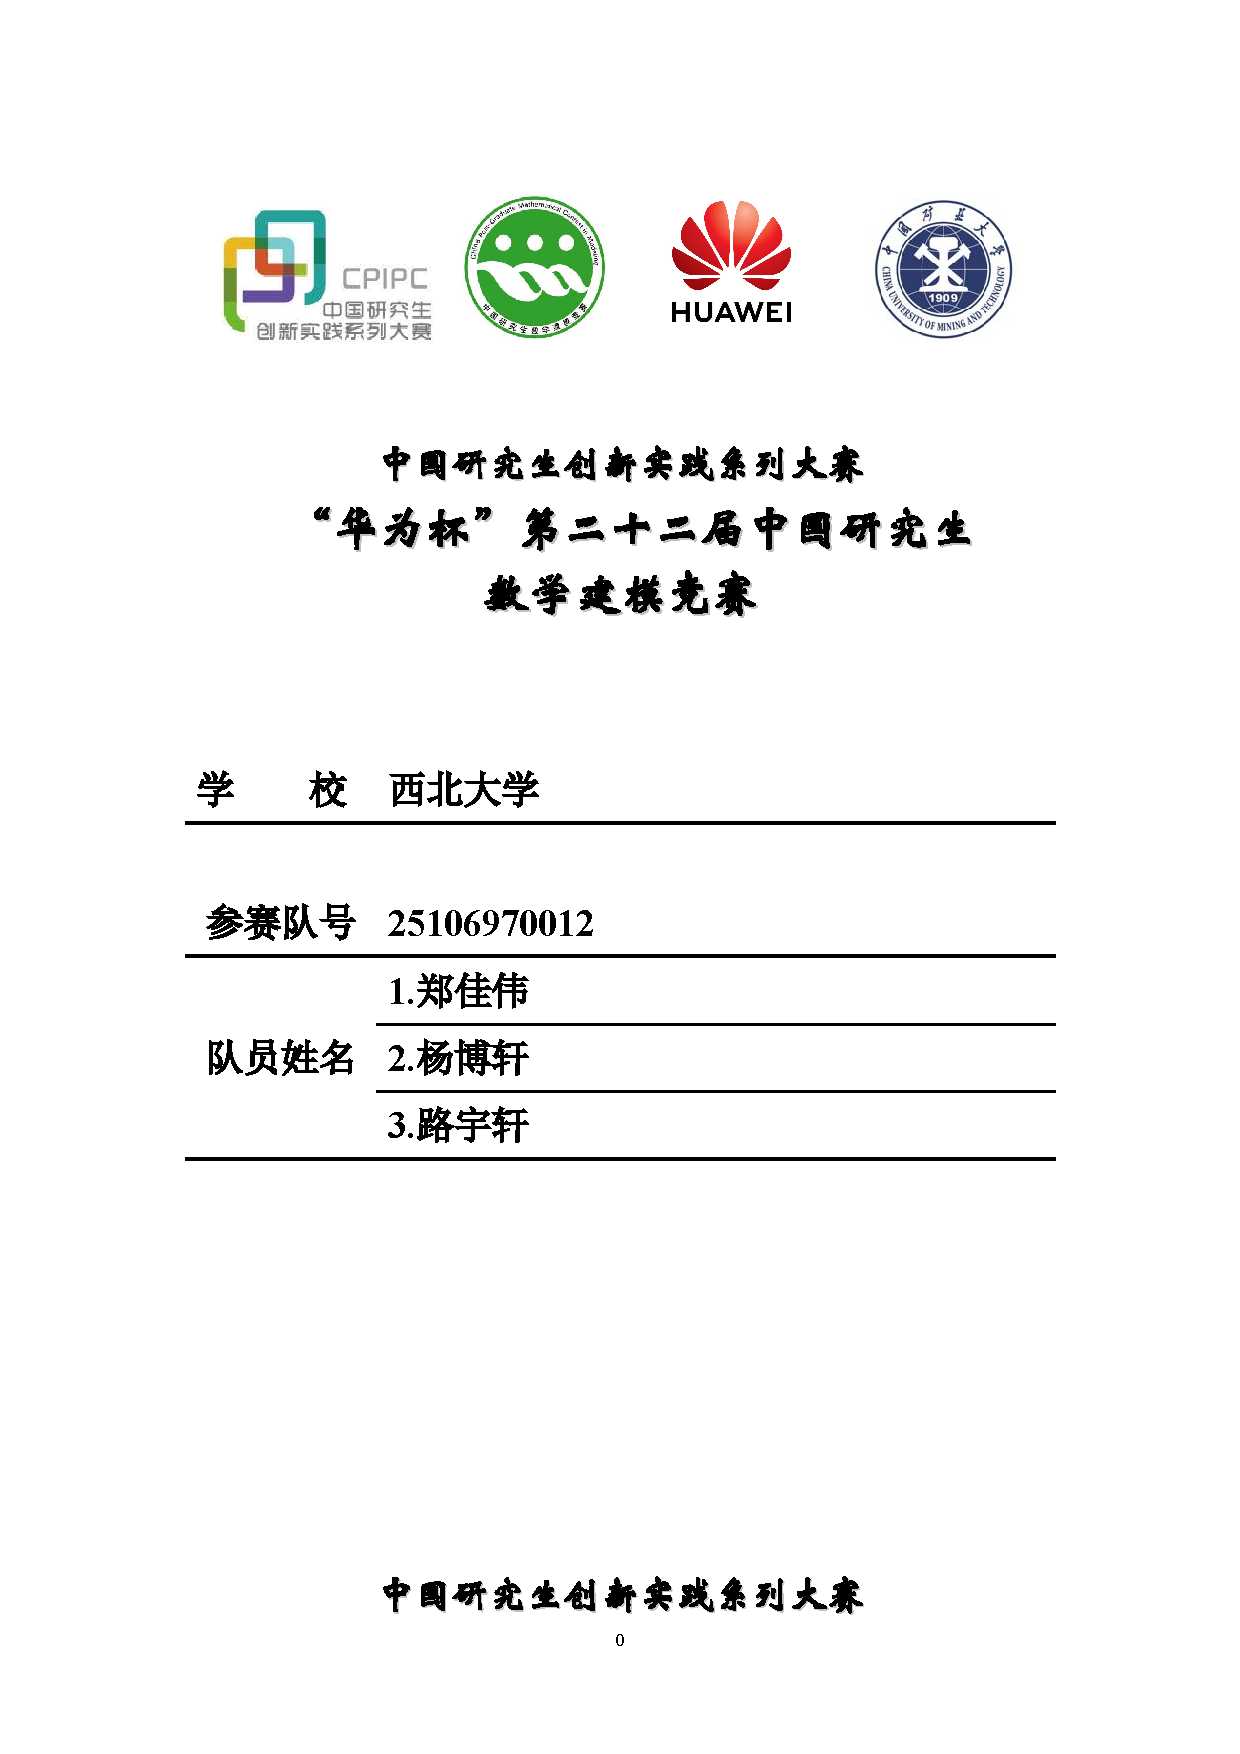
\includepdf[width=21cm]{论文封面}

%--------------------题目&摘要页----------------------
\newpage
\pagenumbering{arabic} %设置阿拉伯数字页码
\setcounter{page}{1} %正文为第一页

\begin{center}
     \zihao{-2}  \shadowtext{\textbf{ \xinwei  中国研究生创新实践系列大赛}}
     \\
    \zihao{2} \shadowtext{\textbf{ \xinwei  “华为杯”第二十二届中国研究生}}

    \zihao{2} \shadowtext{\textbf{\xinwei 数学建模竞赛}}
    \end{center}

\vspace{1em}
\begin{tabular}{l p{0.8\textwidth}<{\centering}}
    \centering
    \zihao{-2} {\textbf{{题\quad 目 :}}}\qquad & \zihao{3} \heiti 高速列车轴承智能故障诊断问题 \\ \cline{2-2}
\end{tabular}
\\
\begin{center} \zihao{-2}  摘 \quad 要:
\end{center}   


\indent  
随着人们对于出行安全意识的不断提高,高速列车故障问题已然成为成国民关注度最高的问题。高速列车轴承是关键且易损的部件,其故障引发的恶性事故通常不可逆转。现有传统诊断方法难以适应复杂运营工况下对精度、泛化性及实时性的高要求,此外,采集的故障信号易受强噪声干扰,会削弱故障特征的显著性。因此建立高效的轴承故障诊断模型具有非常重要的现实意义。本文围绕轴承故障诊断的迁移学习问题,提出了一套完整的解决方案。首先,针对源域与目标域的数据差异,采用阶次分析对齐转速影响,并结合轴承故障机理提取\textbf{时域、频域及包络域等多维度物理特征}。进而,在源域上基于\textbf{随机森林}构建高精度诊断模型\cite{ref1}。随后,通过\textbf{线性域自适应(TCA)}进行域间特征对齐,并结合\textbf{伪标签自训练}策略增强模型在目标域上的适应性。最终,本文构建了涵盖事前特征漂移分析、迁移路径可视化与事后决策归因的多层可解释性框架,实现了模型输出与轴承故障物理机理的显式关联。



问题一$(1)$属于\textbf{特征分析}问题。我们首先将源域中的原始信号统一重采样至与目标域相匹配的带宽,并进行去趋势与带通滤波,之后进行了源域和目标域转速的归一化处理。我们对不同故障类型在频域上进行\textbf{FFT},通过相应频域图去分析在轴承不同位置发生的三种故障有何特点。

问题一$(2)$属于\textbf{特征提取}问题,通过分析上一问的频谱图,我们构建了在时域、频域、包络域、包络域对齐的指标,这对我们判断故障类型有很大帮助。接着我们对这些指标进行重要性排序,从而提取我们需要的特征。

问题二要求我们在问题一已提取的故障特征基础上,进行故障分类以及重要特征的优化。首先我们将全部故障特征数据划分为训练集与测试集。之后我们选取了三种典型机器学习模型进行对比实验。通过综合评估各模型在测试集上的分类准确率和F1得分,我们得出\textbf{随机森林}模型在故障特征重要性排序任务中表现最优。

问题三属于\textbf{迁移诊断}问题。首先,基于问题二构建的诊断模型,采用\textbf{线性域自适应(TCA)}算法对齐源域与目标域特征分布,实现特征空间适配;随后,结合对齐后的源域数据及目标域\textbf{伪标签}数据重新训练分类器,并直接应用于目标域无标签数据分类;最后,通过t-SNE进行特征分布可视化,成功实现了模型知识的稳健迁移。

问题四的关键是解决问题三中模型的“黑箱”问题。我们构建了一套“事前一过程一事后”三层可解释性体系。首先在事前阶段,我们通过对比源域与目标域特征的统计分布差异,识别与轴承故障机理相关的关键特征漂移。其次在迁移过程中利用可视化TCA变换对特征空间的几何调整作用。最后在事后决策阶段,我们采用特征重要性排序和局部归因方法,揭示了模型诊断决策所依赖一系列物理证据。


\vspace{1em}
\noindent  \zihao{-2}\textbf{{关键词:}} \zihao{5} \textbf{FFT;随机森林模型; 线性域自适应(TCA); 伪标签自训练}



%--------------------目录----------------------
\newpage

\begin{center}
\tableofcontents
\end{center}

% \begin{center}
% \tableofcontents
% \setcounter{page}{0}
% \thispagestyle{empty}
% \end{center}

%--------------------正文----------------------
%--------------------问题重述----------------------
\newpage
\section{问题重述}

\subsection{问题背景}

凭借安全高效、便捷舒适以及绿色低碳等显著优势,高速列车已然成为中国客运领域的核心运输工具。
高速列车轴承是关键但易损部件,其故障轻则延误,重则导致恶性事故。
现有基于专家经验或传统信号处理的诊断方法难以满足复杂运营场景下对精度、泛化性和实时性的高要求。
虽然基于深度学习的智能诊断前景广阔,但实际应用中面临两大关键挑战:一是真实运行中传感器采集的振动信号受强噪声干扰,削弱了故障特征;二是出于安全考虑,列车故障会被及时处理,导致可用于训练的真实故障数据极其稀缺,造成数据严重匮乏和分布失衡,阻碍了模型的实际应用。


\subsection{问题提出}
为解决真实故障数据稀缺的问题,题目引入迁移学习技术。其核心思路是利用在试验台架环境采集的、故障机理相似但数量丰富、标签完备的轴承振动数据训练模型,然后将学习到的知识迁移应用到真实列车运行的少量无标签数据上。
通过对所提供的源域数据集和目标域数据集的评估,可以确定以下关键问题需要解决:

\textbf{问题1($1$): 获取指定的轴承试验台架振动数据,并对数据进行预处理和特征分析}

考虑到目标域数据的采样频率与列车实际转速特性,本研究首先将源域12kHz与48kHz采样的原始信号统一重采样至与目标域 32kHz相匹配的带宽,并进行去趋势与带通滤波,以消除低频漂移及高频环境噪声。

\textbf{问题1($2$):结合轴承故障机理提取多维度特征}

首先,在时域中计算均方根值、峭度、峰值因子等统计指标以表征冲击脉冲强度;另外,在频域中通过包络解调获取包络谱,并计算与三种故障特征频率相关的幅值与能量占比,并对这些特征进行提取。



\textbf{问题2:构建合适的模型进行故障分类}

我们将所有特征数据按$80\%$训练集和$20\%$测试集进行随机划分,确保模型训练与评估的有效性。通过对比三种典型机器学习模型发现,随机森林在分类准确率和特征重要性排序方面表现最优,验证了其处理多维特征的优势,为后续故障诊断提供了可靠依据。

\textbf{问题3:使用线性域自适应(TCA)对齐源于数据和目标域数据,然后利用随机森林模型进行分类}

首先利用任务2的模型提取特征,通过TCA对齐源域与目标域的分布,并基于对齐后的数据训练分类器,最终应用于目标域分类。t-SNE可视化表明,该方法有效缩小了域间差异,提升了目标域诊断准确率,实现了稳健的知识迁移。


\textbf{问题4:构建“事前一过程一事后”三层可解释性体系对问题三的“黑箱”问题进行解释}

本文从事前、迁移过程、事后三个维度,结合轴承故障机理与可视化手段,分析任务三模型的可解释性,让诊断人员能清晰理解模型工作逻辑、知识迁移路径及决策依据。

\newpage


%--------------------模型假设----------------------
\section{模型假设与符号说明}
\subsection{模型假设}
考虑到实际问题的复杂性,为简化模型并聚焦于迁移诊断的核心机制,我们作出以下合理假设:

假设 1: 源域与目标域轴承的故障物理机理相同,即同一类型故障在振动信号中激发的特征频率及其调制模式是一致的。

假设 2: 源域与目标域的条件分布 P(y∣x) 保持一致。这意味着,给定相同的故障特征,其在源域和目标域中对应的故障类别标签是一致的。

假设 3: 振动信号中的噪声主要为加性高斯白噪声,且通过本文采用的预处理方法可被有效抑制,使其不主导故障特征的提取与模型的决策。

假设 4: 从源域数据中提取的时域、频域及包络域特征能够充分表征轴承的健康状态,并且这些特征中包含一部分在跨域迁移后仍具有判别力的“域不变特征”。

假设 5: 目标域数据虽无标签,但其数据分布是平滑且连续的,不存在未知的、与源域故障模式完全不同的全新故障类型,从而保证基于源域知识的迁移是可行的。
\subsection{符号说明}
%--------------------符号说明----------------------
\begin{center}
    \begin{tabular}{c | c}
        \toprule[1.5pt]
        \makebox[0.3\textwidth][c]{符号} & \makebox[0.4\textwidth][c]{意义} \\
        \midrule[1pt]
        $BP_{LOW}$      &Butterworth滤波器下限\\
        $BP_{HIGH}$     &Bassworth滤波器上限\\
        $DE$            &驱动端加速度数据\\
        $FE$            &风扇端加速度数据\\
        $BA$            &基座加速度数据\\
        $RPM$           &转/每分钟,除以60为旋转频率\\
        $BPFO$           &外圈故障特征频率\\
        $BPFI$           &内圈故障特征频率\\
        $BSF$            &滚动体故障特征频率\\
        $FSF$            &滚动体公转频率\\
        $K_e$            &包络峭度\\
        $TCA$           &线性域自适应对齐\\
      
    \end{tabular}
\end{center}



%--------------------问题一的分析与求解----------------------
\newpage
\section{问题一的分析与求解}
\subsection{问题一的任务分析}
 \subsubsection{问题一$(1)$的任务分析}
 %\
 对于问题一$(1)$,我们已知源域数据集中包含有DE、FE、BA等数据,题目要求选择合适的方法或指标对有代表性的数据进行特征分析。
 基于所提供的数据,针对源域与目标域的采样频率差异,我们先对源域振动信号进行去趋势、带通滤波,再统一重采样至32kHz以匹配目标域时间尺度;之后我们对不同故障类型进行时域和频域分析,确定其具有物理意义明确的特征: 。

 \subsubsection{问题一$(2)$的任务分析}
 对于问题一$(2)$,我们在问题一$(1)$中已经分析出来的数据特征的基础上,结合轴承故障机理提取多维度特征:一方面,在时域中计算均方根值、峭度、峰值因子等统计指标以表征冲击脉冲强度;另一方面,在频域通过Hilbert包络解调获取包络谱,并计算与BPFL、BPFO及BSF等理论故障特征频率及其旁带相关的幅值与能量占比,以捕捉局部缺陷所引起的周期性冲击。
 
\subsection{基于阶次分析的域自适应数据预处理方法}

数据预处理的核心是跨域信号对齐与故障特征增强。题中源域数据采样频率为12kHz或48kHz,目标域为32kHz,我们需通过重采样将源域数据调整至32kHz,确保时间尺度一致,避免因采样率差异导致的特征偏移。

设原始信号  
$x[n], n = 0, 1, \dots, N - 1$,
$l[n]$为线性拟合,我们通过使用线性拟合可移除信号中的线性趋势分量;
\begin{align}
    \left\{
    \begin{aligned}
    l[n] &= \alpha \cdot n + \beta\\
    \alpha &= \frac{\sum_{n=0}^{N-1} n \cdot x[n] - \frac{1}{N} \left( \sum_{n=0}^{N-1} n \right) \left( \sum_{n=0}^{N-1} x[n] \right)}{\sum_{n=0}^{N-1} n^2 - \frac{1}{N} \left( \sum_{n=0}^{N-1} n \right)^2}\\
    \beta &= \frac{1}{N} \sum_{n=0}^{N-1} x[n] - \alpha \cdot \frac{1}{N} \sum_{n=0}^{N-1} n
   \end{aligned} 
    \right.
\end{align}
我们通过最小二乘法$ y = mx + c $拟合并移除信号中的线性分量,消除基线漂移现象,使信号均值归零。这能有效克服传感器零点漂移或温度变化引起的干扰,从而得到我们需要的去趋势信号  $x_d[n] = x[n] - l[n]$,

接下来我们使用Butterworth滤波器保留特定频段的有效信号成分。通带范围预设为$[BP_{LOW}, BP_{HIGH}]$,其中$BP_{LOW}$设置为500hz,$BP_{HIGH}$设置为10000hz,滤波器表达函数$H(z)$为如下公式:
\begin{align}
 H(z) = \frac{\sum_{k=0}^{M} b_k z^{-k}}{1 + \sum_{k=1}^{N} a_k z^{-k}} 
\end{align}
其中M为分子阶数,N分母阶数,$b_k$,$a_k$由Butterworth原型滤波器计算得到。采用双向滤波(filtfilt)方法消除相位失真,优化边界处理,确保关键波形特征并保持信号完整。

由于源域和目标域转速的显著差异,相同的故障特征在振动信号频率轴上会出现在完全不同的频率点,导致在源域上训练的诊断模型在目标域上性能急剧下降。我们提出了一种基于阶次分析的数据预处理方法,将振动信号从频率域转换到阶次域,从而在本质上消除转速的影响,为后续的迁移学习算法奠定坚实的基础。

阶次分析是一种将振动信号与旋转轴转速相关联的信号处理技术。其核心思想是使用“阶次”作为基准单位,其中1阶次对应轴每旋转一周发生一次的振动分量。因此,一个故障特征在任意转速下都将稳定地出现在固定的特征阶次上,而与转速绝对值无关\cite{ref2}。

对于给定的瞬时转速(RPM),其转频$f_r$(单位:Hz)为
\begin{align}
 f_r = \frac{\text{RPM}}{60} 
\end{align}
那么,信号中任一频率分量f(单位:Hz)对应的阶次O定义为:
\begin{align}
 O = \frac{f}{f_r} 
\end{align}
该公式实现了从频率标尺到阶次标尺的线性映射。例如,一个在1700 rpm(fr≈28.3Hz)下出现在240Hz的故障成分,其阶次为240/28.3≈8.5。在600rpm(fr=10Hz)下,表征同一故障的成分将出现在8.5×10=85Hz。通过阶次分析,两个不同转速下的同一故障成分都被映射到了8.5阶,实现了故障特征的转速归一化对齐。


\subsection{源域数据的特征分析}
\subsubsection{时域信号分析}

轴承故障诊断技术,核心是通过实时监测轴承运行状态下的各类特征信号(其中振动加速度信号因能直观反映轴承机械结构的异常振动,是最主要的监测数据),结合数据挖掘、信号处理及机器学习等技术手段,对监测数据进行分析与特征提取,最终精准判定轴承是否存在故障、故障类型及故障严重程度,为列车轴承的预防性维护提供科学依据。

轴承结构主要包括内圈、外圈、滚动体和保持架四部分,其中典型故障多发生在内圈、外圈和滚动体这三个核心承载部件。我们可以看到当三种部件出现单一缺陷时,传感器采集到的周期性振动冲击示意图如下所示。
\begin{figure}[H]
  \centering
  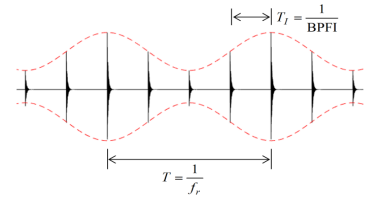
\includegraphics[width=0.6\textwidth]{内圈故障示意图.png}
  \caption{内圈故障示意图}
  \label{fig:confidence}
\end{figure}\begin{figure}[H]
  \centering
  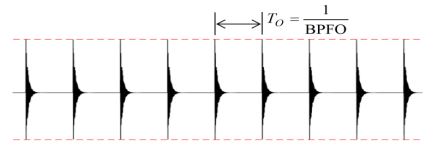
\includegraphics[width=0.6\textwidth]{外圈故障示意图.png}
  \caption{外圈故障示意图}
  \label{fig:confidence}
\end{figure}\begin{figure}[H]
  \centering
  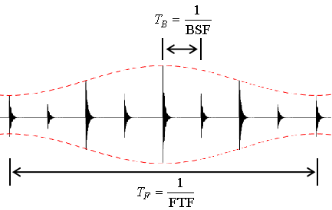
\includegraphics[width=0.6\textwidth]{滚轴体故障示意图.png}
  \caption{滚轴体故障示意图}
  \label{fig:confidence}
\end{figure}
当外圈出现故障时,其时域信号表现为固定时间间隔的冲击序列,冲击间隔${T_0} =  \tfrac{1}{BPFO}$。这是由于外圈与轴承座固定,不随转子旋转,DE端采集的信号直接来自外圈故障部位,振动传递路径短,故障信号幅值明显。

当内圈出现故障时,其时域信号表现为带幅度调制的冲击序列,冲击间隔${T_I} =  \tfrac{1}{BPFI}$,且冲击幅度随时间呈周期性波动。这是因为内圈与转子轴固定,随转子旋转,而载荷方向不变,内圈故障点每次通过载荷区时,故障点与滚动体的接触位置随内圈旋转而变化,导致冲击强度周期性变化。

当滚动体出现故障时,其时域信号表现为双重幅度调制的冲击序列,冲击间隔${T_B} =  \tfrac{1}{BSF}$,且冲击峰值的包络线同时包含BSF的高频振荡
FTF的低频波动,形成“嵌套波浪形”时域特征。这是因为故障滚动体与内圈、外圈的接触位置随公转和自转周期性变化,导致冲击强度双重调制。故障信号需通过内圈、外圈传递至驱动端,因此幅值比外圈故障小,但调制特征更明显\cite{ref3}。

根据轴承几何参数可以得到三种故障的特征频率计算公式如下:
\begin{align}
    \left\{
    \begin{aligned}
    BPFO &= f_r \cdot \frac{N_d}{2} \cdot \left(1 - \frac{d}{D}\right) \\
    BPFI &=f_r \cdot \frac{N_d}{2} \cdot \left(1 + \frac{d}{D}\right)    \\
    BSF  &=f_r \cdot \frac{D}{d}\left[1 - \left(\frac{d}{D}\right)^2\right]\\
    \end{aligned} 
    \right.
\end{align}
其中, $f_r = \frac{n}{60}$ 为轴承转频,$n$为轴承内圈转速(单位:rpm),$d$为滚动体直径,$D$为轴承节径(通常可由$\frac{\text{内径} + \text{外径}}{2}$估算),$N_d$为滚动体个数。

由公式可以看出,三种故障的特征频率完全不同,导致其在频域中的峰值不同,所以我们可以根据峰值位置直接区分故障类型,这是时域特征无法替代的。

\subsubsection{频域信号分析}

由于轴承故障的本质是周期性冲击,这些冲击会产生固定的特征频率。但是时域信号无法直接分离这些特征频率:三类故障的时域波形均为冲击信号,但内圈故障有幅度调制、滚动体故障有双重调制,导致时域波形相似,难以区分。而快速傅里叶变换(FFT)能将时域信号转换为频域频谱,使特征频率以峰值形式清晰呈现。

我们利用FFT分析三种故障的频域特征,并通过带通滤波(如过滤4~6 kHz的共振频率带)和包络分析,可突出特征频率峰值,抑制噪声。

当轴承正常时驱动端和风扇段的频域特征如图所示:

\begin{figure}[H]
  \centering
  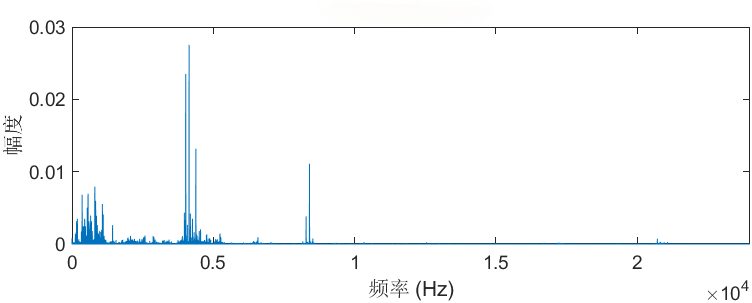
\includegraphics[width=0.6\textwidth]{正常风扇端.png}
  \caption{正常风扇端}
  \label{fig:confidence}
\end{figure}
\begin{figure}[H]
  \centering
  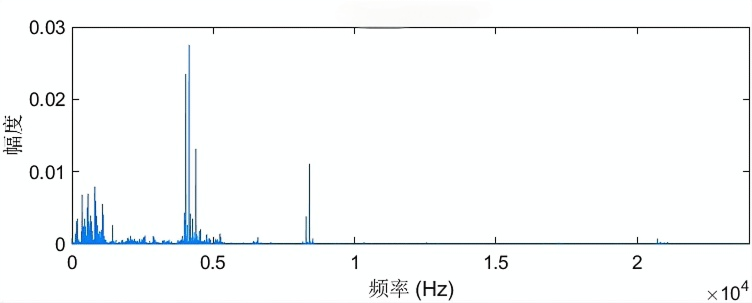
\includegraphics[width=0.6\textwidth]{正常驱动端.png}
  \caption{正常驱动端}
  \label{fig:confidence}
\end{figure}

由图4,5可以看出,正常情况下信号的频谱图频谱无明显故障特征频率,背景噪声低,频谱结构整齐、无突兀峰值。正常轴承的振动主要来自转子旋转的不平衡激励和轴承滚动体的正常滚动摩擦,因此频谱的低频率段(0-1kHz)会出现旋转频率及其谐波,且谐波幅度随频率升高逐渐衰减。而在4-6kHz附近出现高幅度谐波主要由驱动端结构的固有共振频率引起,导致该频率附近的幅度显著高于其他中高频成分,是正常情况下传动系统激励的结果,在8kHz附近的高幅度并非机械振动的固有特征,而是传感器或采集电路的高频噪声,属于系统误差范围之内。

当滚轴体出现故障时驱动端、风扇端、基站端的频域特征如图所示:
\begin{figure}[H]
  \centering
  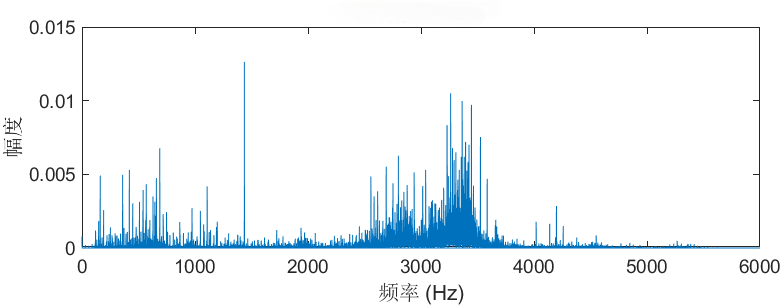
\includegraphics[width=0.6\textwidth]{滚轴体问题驱动端.png}
  \caption{滚轴体问题驱动端}
  \label{fig:confidence}
\end{figure}
\begin{figure}[H]
  \centering
  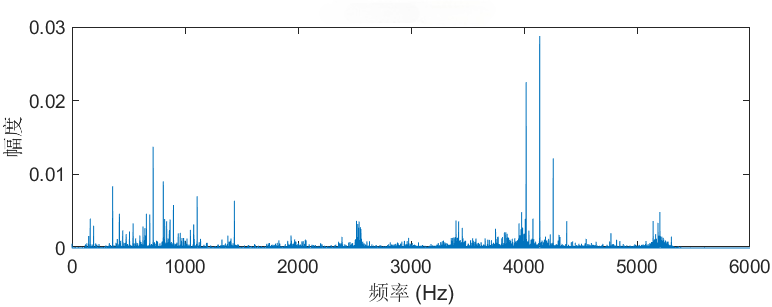
\includegraphics[width=0.6\textwidth]{滚轴体问题风扇端.png}
  \caption{滚轴体问题风扇端}
  \label{fig:confidence}
\end{figure}
\begin{figure}[H]
  \centering
  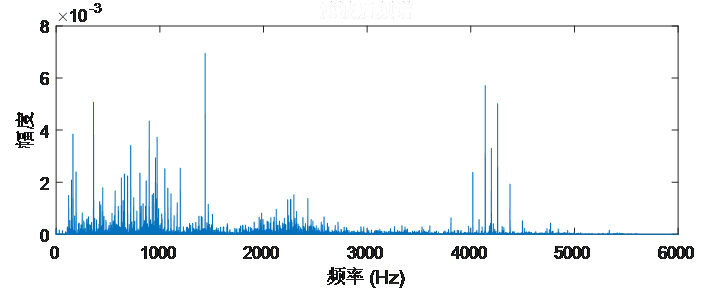
\includegraphics[width=0.6\textwidth]{滚轴体基站端.png}
  \caption{滚轴体基站端}
  \label{fig:confidence}
\end{figure}


我们在DE端使用的轴承类型为SKF6205,其滚动体数${N_d=9}$,滚动体直径${d=0.3126英寸}$,轴承节径${D=1.537英寸}$。所以根据图6和公式3.5可以算出$DE_{BSF}$约等于140hz。

滚动体故障时,滚动体的公转运动会对BSF信号产生幅度调制,导致BSF峰值两侧出现边带,边带间隔等于滚动体公转频率(Fundamental Train Frequency, FTF),公式为:
\begin{align}
   \text{FTF} \approx f_r \cdot \left(1 - \frac{d}{D}\right)
\end{align}
计算可得FTF=23.8Hz。边带间隔由FTF决定,源域边带间隔约23.8Hz(如140±23.8Hz→116.2Hz、163.8Hz)。边带的存在验证了滚动体的“公转+自转”运动,是区分滚动体故障与其他故障的重要依据。

在3000-4000Hz内共振频带的边带幅值远高于低频率段的BSF主峰值,这是因为驱动端直接连接电机转轴,结构刚度大,其固有共振频率会放大滚动体故障的冲击信号,导致频域图中共振频带内的边带幅值显著升高,此边带可以提升滚动体故障诊断精度。

我们在FE端使用的轴承类型为SKF6203,其滚动体数${N_d=9}$,滚动体直径${d=0.2656英寸}$,轴承节径${D=1.122英寸}$。。所以由图7和公式3.5我们可以算出$FE_{BSF}$约等于120hz。风扇端的结构固有频率通常位于中高频率段。滚动体故障的宽带冲击信号会激发该频段的共振,所以会导致在3700-4200hz频段内的BSF边带幅值显著升高。

综上可知,我们可以根据在频谱图中不同频域范围内的峰值来区分三类故障。

当内圈出现故障时驱动端、风扇段、基站端的频域特征如图所示:

\begin{figure}[H]
  \centering
  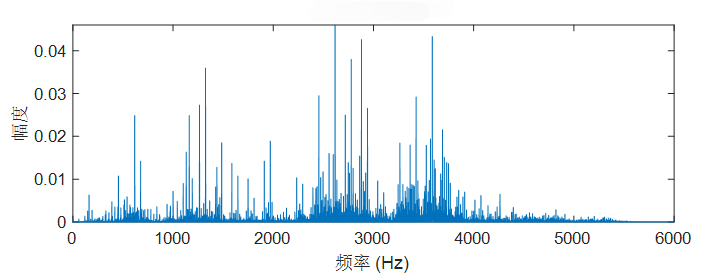
\includegraphics[width=0.6\textwidth]{内圈故障驱动端.png}
  \caption{内圈故障驱动端}
  \label{fig:confidence}
\end{figure}
\begin{figure}[H]
  \centering
  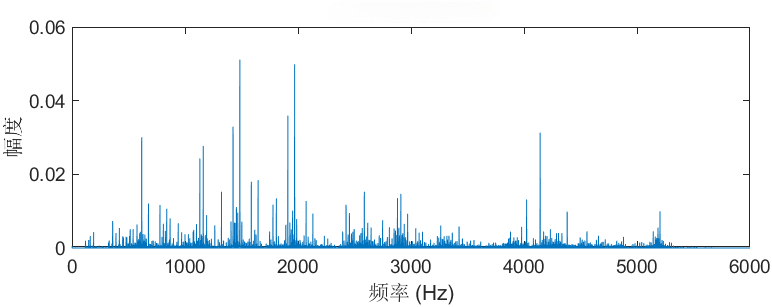
\includegraphics[width=0.6\textwidth]{内圈故障风扇段.png}
  \caption{内圈故障风扇端}
  \label{fig:confidence}
\end{figure}
\begin{figure}[H]
  \centering
  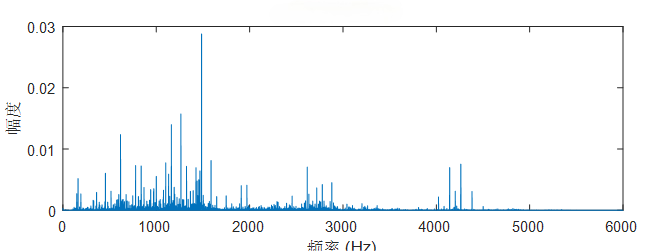
\includegraphics[width=0.6\textwidth]{内圈故障基站端.png}
  \caption{内圈故障基站端}
  \label{fig:confidence}
\end{figure}


根据图9和公式3.5,可以计算出$DE_{BPFI}$=162Hz。在低频率段(0-200Hz),BPFI及其谐波的峰值明显,幅值远高于正常状态,其边带呈对称分布。而在中高频率段(2000-4000Hz)出现了大规模的高幅值边带,这是由于故障冲击激发驱动端结构共振所致。

根据图10和公式3.5,可以计算出$FB_{BPFI}$=55.7Hz,该频率由风扇端轴承几何参数唯一确定,是识别内圈故障的标志性特征。FE端内圈故障的频谱在较高频率段(500-2000Hz)幅值显著高于正常状态,500-1000Hz之间有次高幅值峰值(如超过0.03的峰值),1000-2000Hz之间有高幅值峰值,这些均为内圈故障的典型特征。


当外圈出现故障时驱动端、风扇段、基站端的频域特征如图所示:
\begin{figure}[H]
  \centering
  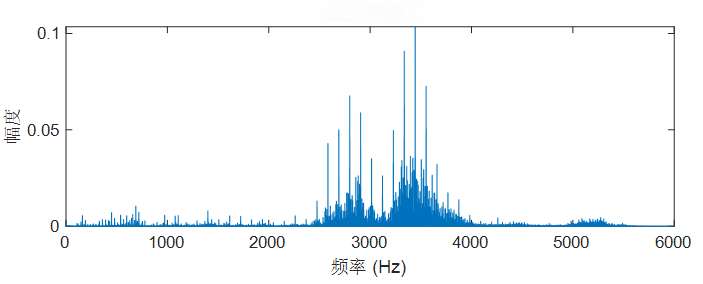
\includegraphics[width=0.6\textwidth]{外圈故障驱动端.png}
  \caption{外圈故障驱动端}
  \label{fig:confidence}
\end{figure}\begin{figure}[H]
  \centering
  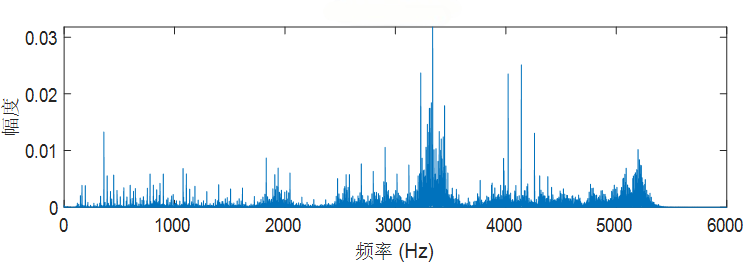
\includegraphics[width=0.6\textwidth]{外圈故障风扇端.png}
  \caption{外圈故障风扇端}
  \label{fig:confidence}
\end{figure}\begin{figure}[H]
  \centering
  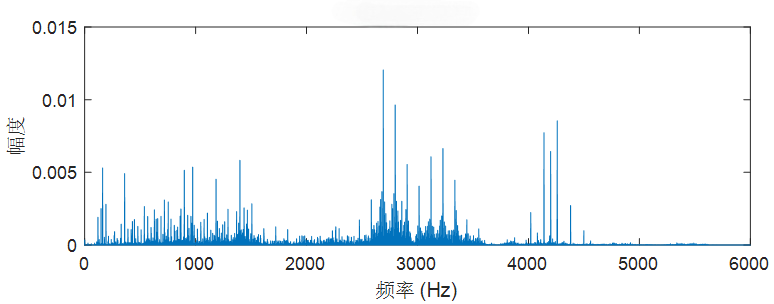
\includegraphics[width=0.6\textwidth]{外圈故障基站端.png}
  \caption{外圈故障基站端}
  \label{fig:confidence}
\end{figure}
根据图12和公式3.5,可以计算出$DE_{BPFO}$=35.8Hz。图中2000-4000Hz之间有高幅值峰值(如2600Hz左右超过0.07的峰值、3800Hz左右超过0.09的峰值),这些共振边带是故障信号的“放大器”

根据图13和公式3.5,可以计算出$FE_{BPFO}$=34.35Hz。图中2000-4000Hz之间有高幅值峰值(如2000Hz左右超过0.01的峰值、3500Hz左右超过0.03的峰值、4000Hz左右超过0.02的峰值),这些共振边带可以放大故障信号,即使风扇端传递路径长,也能清晰识别故障特征。

\subsection{源域数据的特征提取}
由于原始振动数据是高维度、高冗余的,直接用于模型训练会导致计算效率低,我们根据FFT进行频域分析,将原始数据转换为低维度、高信息密度的特征,可以保留故障的核心信息。我们根据以下四个方面进行论述:
\subsubsection{时域统计}
轴承故障的核心时域特征是周期性冲击脉冲。时域统计指标通过量化信号的幅值分布、离散程度、峰值特性,捕捉冲击脉冲的强度、频率和对称性。以下是常用指标的定义、计算方法及故障机理关联:

\begin{enumerate}
    \item 均值(Mean):信号的平均水平,可反映传感器偏置或缓慢漂移;公式如下:
     \begin{equation}
      \mu = \frac{1}{N} \sum_{i=1}^{N} x_i
    \end{equation}
    $\{x_i\}_{i=1}^{N}$表示离散振动信号,理想振动的$\mu$应接近0。故障时,冲击脉冲会使信号的交流分量增加,但均值受直流分量影响大,因此对故障不敏感
    \item 标准差(Std):信号偏离均值的离散程度,反映信号的波动大小;公式如下:
     \begin{equation}
       \sigma = \sqrt{\frac{1}{N - 1} \sum_{i=1}^{N} (x_i - \mu)^2}
    \end{equation}
    故障时,冲击脉冲会增加信号的幅值波动,因此标准差增大
    \item 均方根值(RMS):信号的有效值,反映信号的总能量;公式如下:
    \begin{equation}
        \text{RMS} = \sqrt{\frac{1}{N} \sum_{i=1}^{N} x_i^2}
    \end{equation}
    故障特征:故障时,冲击脉冲的能量增加,因此RMS显著增大
    \item 峭度(Kurtosis):信号的峰值特性,反映极端值的出现概率;公式如下:
    \begin{equation}
        K = \frac{1}{N} \sum_{i=1}^{N} \frac{(x_i - \mu)^4}{\sigma^4} 
    \end{equation}
    峭度是轴承故障的核心敏感指标。冲击脉冲会导致信号出现尖峰,峭度远大于3(正常状态K≈3)
    \item 峰值因子(CF):峰值与RMS的比值,反映冲击脉冲的陡峭程度;公式如下:
    \begin{equation}
       \text{CF} = \frac{P}{\text{RMS}}
    \end{equation}
    P是峰值。故障时,冲击脉冲的峰值增长快于RMS,因此峰值因子增大
    \item 脉冲因子(IF):峰值与绝对值均值的比值,反映冲击脉冲的强度;公式如下:
     \begin{equation}
       \text{IF} = \frac{P}{\frac{1}{N} \sum_{i=1}^{N} |x_i|}
    \end{equation}
    故障时,冲击脉冲的峰值增大,而绝对值均值变化小,因此脉冲因子显著增大。
    \item 间隙因子(CLF):峰值与绝对值均值平方根的比值,反映冲击脉冲的稀疏程度;公式如下:
     \begin{equation}
       \text{IF} = \frac{P}{\frac{1}{N} \sum_{i=1}^{N} |x_i|}
    \end{equation}
    间隙因子强调尖峰对低阶统计的支配程度;对微小局部缺陷的早期冲击尤敏感。故障时,冲击脉冲的间隔缩短,因此间隙因子增大
\end{enumerate}

根据对以上时域特征的分析,我们优先选择对故障敏感,且受转速影响小的特征:峭度、峰值因子、脉冲因子;

\subsubsection{频域统计}

我们首先需要通过重采样将源域采样率与目标域采样率统一,以及源域转速与目标域转速的一致。当源域采样率为12kHz时,使用样条插值补充高频成分,保持时间序列连续性,使其提升到目标域所需的采样率32kHz;当源域采样率为48kHz,先使其通过低通滤波器,再用降采样至32kHz。之后使用Hilbert包络解调可突出冲击的包络频率,具体操作为对预处理后的时域信号x(t)做FFT,得到幅值谱X(f),之后根据公式$ S(f) = |X(f)|^2 $求出功率谱密度,最后根据公式$ P(f) = \frac{S(f)}{\sum |S(f)|} $对功率谱密度进行归一化,将各频率成分的功率占比反映出来。
我们提取到的频域统计特征如下:
\begin{enumerate}
    \item 主频(Dominant Frequency):功率谱中幅值最大的频率点及其幅值;公式如下:
     \begin{equation}
       f_{\text{dom}} = f_{k^*}, \\
       k^* = \arg\max_{k} |X_k|
    \end{equation}
    故障时,主频会向理论故障频率偏移,其中,理论故障频率指的是三种故障特征频率(BPFO、BPFI、BSF)。
    \item 谱质心(Spectral Centroid):谱能量的集中位置;公式如下:
     \begin{equation}
        C = \sum_{k} f_k p_k 
    \end{equation}
    故障时,主频会向理论故障频率偏移
    \item 谱熵(Spectral Entropy):谱分布的均匀性;公式如下:
     \begin{equation}
         H = -\sum_{k} p_k \ln p_k 
    \end{equation}
    故障时,谱能量集中在理论故障频率,谱熵减小
    \item 谱带宽(Spectral Bandwidth):谱能量的分散程度;公式如下:
     \begin{equation}
        C = \sum_{k} f_k p_k 
    \end{equation}
    故障时,谱能量集中在理论故障频率,谱带宽减小
\end{enumerate}

\subsubsection{包络域统计}
由于轴承局部故障会产生周期性冲击信号,这些冲击会对原始振动信号进行调幅(Amplitude Modulation, AM)。我们在频域对信号进行Hilbert包络解调可提取幅度分量,消除原始信号中的载波成分,凸显冲击的周期性;还可以对故障的“能量”与“尖锐度”进行量化。其中包络域统计的两个主要特征:包络$RMS_e$和包络峭度($K_e$)的公式如下
\begin{align}
    \left\{
    \begin{aligned}
     e_i &= |\tilde{x}_i|, \\
     \quad \text{RMS}_e &= \sqrt{\frac{1}{N} \sum_{i=1}^{N} e_i^2}\\
     \quad K_e &= \frac{1}{N} \sum_{i=1}^{N} \frac{(e_i - \bar{e})^4}{\sigma_e^4} 
      \end{aligned} 
    \right.
\end{align}
其中$RMS_e$反映包络信号的能量,故障时,冲击幅值增大,包络RMS显著增加;
包络峭度($K_e$)反映包络信号的尖锐度,周期性冲击的“尖峰”会导致峭度远大于3(正常状态下信号峭度为3),且早期故障的峭度增长更明显。

早期故障的冲击幅值小,时域特征可能被噪声淹没,而包络域特征对周期性冲击的尖锐度极敏感,能在早期故障时显著增大。例如,源域中风扇端滚动体故障的原始信号时域峭度≈4,但包络峭度≈10,出现明显故障,说明包络域特征更适合早期故障诊断。

\subsubsection{包络域对齐指标}
轴承故障所产生的周期性冲击会在理论故障频率处产生包络谱峰值。包络谱对齐指标通过带内索引聚焦于理论故障频率及其周边频段,过滤无关频率,确保特征提取的针对性。带内索引$\quad \mathcal{I}(f_0)$是以理论故障频率f0为中心,宽度为2δ的频段,公式如下:
\begin{align}
    \left\{
    \begin{aligned}
     E_{\text{tot}} &= \sum_{k} |E(f_k)|^2 \Delta f\\
     \quad \mathcal{I}(f_0) &= \{ k : |f_k - f_0| \leq \delta \}     
    \end{aligned} 
    \right.
\end{align}
其中$E_{\text{tot}}$是包络谱的总能量。

包络谱对齐指标通过总能量、带内峰值、能量占比、倍频占比等维度,量化故障的突出程度、能量集中程度和严重程度。带内峰值(Peak)是理论故障频率频段内的最大幅值,直接反映故障冲击的尖锐度;带内能量(BandE)是理论故障频率频段内的能量总和,反映故障冲击的总能量;
能量占比(Eratio)是带内能量与包络谱总能量的比值,标准化后便于不同样本比较;倍频能量(HarmE)是理论故障频率的前M个倍频(默认M=5)能量总和,反映故障的谐波丰富度\cite{ref4}。其具体公式如下:
\begin{align}
    \left\{
    \begin{aligned}
    \text{Peak}(f_0) &= \max_{k \in \mathcal{I}(f_0)} |E(f_k)|\\
    \text{BandE}(f_0) &= \sum_{k \in \mathcal{I}(f_0)} |E(f_k)|^2 \Delta f\\
    \text{Eratio}(f_0) &= \frac{\text{BandE}(f_0)}{E_{\text{tot}}}\\
    \text{HarmE}_M(f_0) &= \sum_{m=1}^{M} \text{BandE}(mf_0)\\
    \end{aligned} 
    \right.
\end{align}
由公式可知:带内峰值(Peak)可直接反映故障冲击的突出程度。源域中,驱动端OR样本的故障尺寸为0.021英寸,其$\text{Peak}(f_0)$远大于0.007英寸样本,模型可通过$\text{Peak}(f_0)$评估故障严重程度;在源域中,正常样本的$\text{Eratio}(f_0)$极低(如0.1,噪声能量占比高),故障样本的高(如0.5,故障能量占比高),模型可通过$\text{Eratio}(f_0)$快速区分正常还是故障;而$\text{HarmE}_M(f_0)$可反映故障的谐波丰富度,故障越严重,激发的倍频越多,$\text{HarmE}_M(f_0)$越大。

    

%--------------------问题二的模型建立与求解----------------------
\newpage

\section{问题二的分析与求解}
\subsection{问题二的任务分析}
根据问题二的要求,我们在问题一已提取的故障特征基础上,构建合适的模型进行故障分类。首先,为保障模型训练与评估的有效性,我们将全部故障特征数据划分为训练集与测试集,采用随机划分策略,以$80\%$的数据作为训练集用于模型学习,$20\%$的数据作为测试集用于性能验证。

为系统比较不同模型在故障特征重要性排序方面的表现,我们选取了三种典型机器学习模型进行对比实验。通过综合评估各模型在测试集上的分类准确率,发现随机森林模型在分类模型中表现最优,其训练后的分类准确率可达$96.96\%$。该结果不仅验证了随机森林在处理多维度特征时的优势,也为其在后续故障诊断中的实际应用提供了可靠依据。

\subsection{数据相关性分析}

我们首先对所有缺失部分进行0填充。我们的数据具有以下几个突出的特点:
首先,信息分布十分分散:故障特征在频域和时域上的分布极不均衡。具体表现为:某类故障往往仅在少数关键频率段或少数时域指标上表现出明显的异常变化,而在其他频率或指标上几乎无差异。这种“稀疏性”意味着若直接使用全部特征进行建模,不仅会增加计算复杂度,还可能引入大量无关噪声,降低模型的泛化能力。
其次,特征往往“成族”出现,同一类故障往往会引发多个相关频率点及其谐波、旁带的协同变化。例如,内圈故障通常会同时引起基频及其2×、3×谐波能量的显著提升。这种“频率族”现象表明,特征之间具有天然的组结构。因此,特征选择方法应具备识别并保留这类成组特征的能力,而非孤立地筛选单个特征。


\subsection{基于随机森林模型的故障分类}

为进一步验证所选特征的有效性,我们同时构建随机森林模型进行故障分类。随机森林作为一种基于多棵决策树集成的规则判别模型,能通过信息熵最小化自动学习特征之间的交互关系,并提供特征重要性排序,增强特征选择的可信度\cite{ref5}。
其流程如下图15所示


\begin{figure}[H]
  \centering
  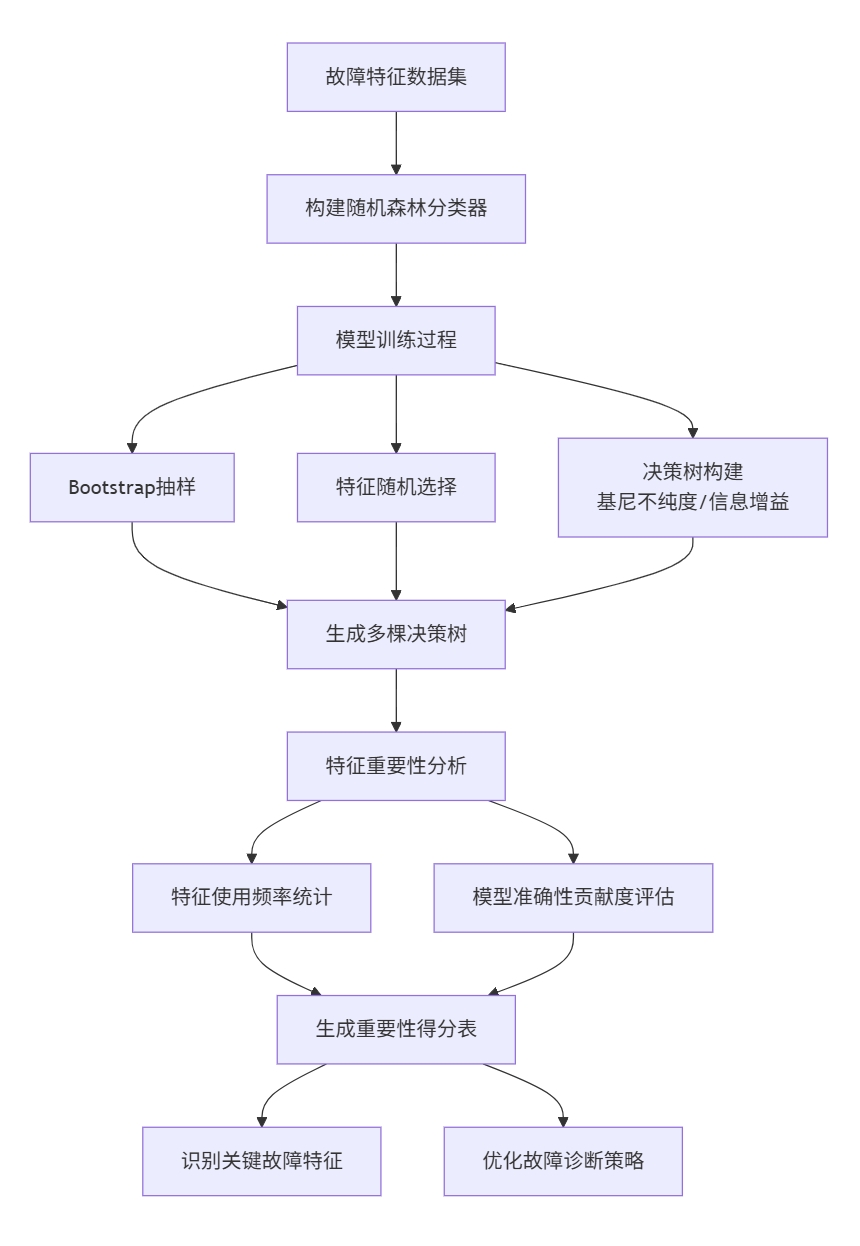
\includegraphics[width=0.6\textwidth]{随机森林流程图.jpeg}
  \caption{随机森林流程图}
  \label{fig:confidence}
\end{figure}


首先,将所有故障特征作为输入特征向量,构建随机森林分类器。通过 Bootstrap 抽样和特征随机选择的方式生成多棵决策树,并利用基尼不纯度或信息增益作为分裂准则。随机森林的关键优势在于:通过“重采样”和“特征随机”减少决策树之间的相关性,从而降低过拟合风险;同时,多个决策树的组合能捕捉高维特征中的非线性模式,比单一决策树更稳定、更鲁棒。

轴承故障分类的核心挑战是从多维度特征中提取故障模式。源域数据需提取时域、频域、包络域等特征,这些特征之间存在非线性关系。随机森林通过多个决策树的组合,能有效捕捉这些非线性模式,避免单一决策树因维度灾难而无法学习。

在模型训练完成后,我们基于特征在随机森林中被使用的频率和其对模型准确性的贡献度,计算每个特征的重要性得分,最终生成故障特征的重要性得分表,以识别对故障分类最具影响力的关键特征。

\subsection{其他模型的故障分类}

\subsubsection{基于CNN+SVM混合模型分析}

为解决复杂工况下故障特征难以有效识别与分类的问题,本研究提出了一种卷积神经网络(CNN)与支持向量机(SVM)相结合的混合诊断模型。传统的端到端CNN模型其末端的Softmax分类器在处理高维、非线性特征时,决策边界可能并非最优。而SVM作为一种基于结构风险最小化的强大分类器,擅长在特征空间中构建最大间隔的超平面,从而获得强泛化能力。因此,本模型利用CNN强大的非线性特征提取能力,自动学习故障信号的本质特征,并交由更专精于分类的SVM进行最终决策,以实现优势互补,提升诊断精度与鲁棒性。

\subsubsection{基于MLP模型分析}

本研究也采用了多层感知器(Multilayer Perceptron, MLP)模型对故障特征进行分类诊断。MLP作为一种经典的前馈神经网络,具备强大的非线性拟合能力,其通用近似特性保证了模型能够从高维特征中学习到有效的判别模式,尤其适用于本研究所涉及的多特征融合的故障分类任务。
MLP由输入层、两个隐藏层和输出层组成,其中输入层维度为$in_{dim}$(对应源域归一化后的特征数量);第一个隐藏层通过nn.Linear($in_{dim}$, h1)实现低级特征提取,其后接ReLU激活函数处理非线性问题,并通过Dropout(0.2)随机丢弃$20\%$神经元,减少模型对源域轻微噪声的依赖;第二个隐藏层通过nn.Linear(h1, h2)实现高级故障模式组合,同样采用ReLU激活与Dropout(0.2)正则化;输出层通过nn.Linear(h2, $num_classes$)映射到4个故障类别。

模型具体配置如下:训练轮数(epochs)设为500以确保模型充分学习故障特征;批次大小(batch size)选取64,平衡了训练效率与梯度估计稳定性;学习率(lr)采用$10^4$的较小值,结合Adam优化器缓慢收敛至最优解,避免因学习率过大跳过极值点;权重衰减(weight decay)设为$10^5$,通过L2正则化缓解源域数据量有限带来的过拟合;dropout率固定为0.2,随机丢弃$20\%$的神经元以减少模型对源域轻微噪声的依赖;测试集比例(test size)设置为0.2,按8:2划分训练与测试集以客观评估泛化能力;随机种子(seed)固定为42,确保数据划分与权重初始化的可重复性。

\subsection{实验结果分析}

我们将以上三种模型训练出来的结果进行了对比分析,得出的结果如表格所示:

\begin{table}[H]
\centering
\caption{不同方法的比较}
\label{tab:method_comparison}
\setlength{\extrarowheight}{2pt}
\begin{tabular}{l| c  c}
    \toprule
        \textbf{Method} & \textbf{Accuracy} $\uparrow$ & \textbf{F1-Score} $\uparrow$ \\
        \midrule
        Random Forest & \cc{1}\textbf{0.9697} & \cc{1}\textbf{0.9758} \\
        CNN + SVM & \cc{2}0.9690 & \cc{2}0.9444 \\
        MLP & \cc{3}0.9394 & \cc{3}0.9243 \\
    \bottomrule
\end{tabular}
\end{table}

\begin{table}[H]
\centering
\caption{根据TopK策略选择的不同特征数量}
\label{tab:topk_results}
\setlength{\extrarowheight}{2pt}
\begin{tabular}{c|c|cc}
    \toprule
    \textbf{k\_or\_thr} & \textbf{kept\_features} & \textbf{Accuracy $\uparrow$} & \textbf{Macro-F1 $\uparrow$} \\
    \midrule
    top10 & 10 num + 0 cat & 0.818181818 & 0.596656611 \\
    top20 & 20 num + 0 cat & \cc{3}0.909090909 & 0.695900178 \\
    top30 & 30 num + 0 cat & \cc{1}0.96969697 & \cc{1}0.975757576 \\
    top40 & 40 num + 0 cat & 0.909090909 & 0.\cc{3}692857143 \\
    top50 & 50 num + 0 cat & \cc{2}0.939393939 & 0.\cc{2}718627451 \\
    top60 & 60 num + 0 cat & 0.96969697 & 0.975757576 \\
    top70 & 70 num + 0 cat & 0.96969697 & 0.975757576 \\
    \bottomrule
\end{tabular}
\end{table}

为评估所提方法的有效性,我们从不同诊断方法的指标进行对比分析:
不同诊断模型在测试集上的性能对比如表1所示:

随机森林(Random Forest)模型取得了最优性能,其准确率达到$96.97\%$,F1分数达到$97.58\%$。CNN+SVM组合模型的准确率可达$96.90\%$与随机森林相近,但其F1分数相对较低,表明其在某些类别上的分类一致性略逊于随机森林。MLP模型的综合性能相对最低,准确率和F1分数分别为$93.94\%$和$92.43\%$。实验结果验证了随机森林模型在处理高维故障特征方面的优势,其集成学习机制有效提升了诊断的鲁棒性和准确性。

综合以上实验结果,本研究最终采用基于Top-30特征选择的随机森林模型作为核心诊断方法,其在保证高精度的同时兼具良好的计算效率。





%--------------------问题三的模型建立与求解----------------------
\newpage
\section{问题三的分析与求解}

\subsection{问题三的任务分析}

针对问题三的迁移诊断任务,本文采用了一种基于线性域自适应对齐(TCA)的无监督域自适应方法。该方法的核心在于识别并缓解源域与目标域之间的特征分布差异(即$(\text{即 } P_s(x) \neq P_t(x))$ ),同时利用其共享的条件分布($P_s(y|x) = P_t(y|x)$)这一关键假设。具体流程是:首先,在问题二构建的基础诊断模型上,提取两域的高维特征;接着,使用TCA算法将源域和目标域对应的重要特征进行对齐,从而在特征空间实现分布适配;对齐后的源域数据用于重新训练分类器,最终将其直接应用于目标域无标签数据进行分类标定。为验证迁移效果,我们采用t-SNE进行特征分布可视化,结果表明该方法能有效缩小域间差异,显著提升目标域上的诊断准确率,成功实现了模型知识的稳健迁移\cite{ref6}。

\subsection{迁移学习}
\subsubsection{特征对齐}
本文提出的迁移诊断模型的核心思想是特征重构,分布对齐。模型工作流程可分为离线训练与在线应用两个阶段。离线阶段,利用带标签的源域数据和无标签的目标域数据共同进行分布对齐,并训练一个适用于目标域特征的分类器;在线阶段,直接将新采集的目标域数据输入训练好的模型,得到诊断结果。

在无监督域自适应领域,线性域自适应(TAC)是一种旨在减少域间分布差异的特征级迁移方法。其核心思想是寻求一个线性映射矩阵$ A \in \mathbb{R}^{d \times d} $,使得源域特征经过该矩阵变换后的协方差矩阵与目标域的协方差矩阵尽可能接近。具体而言,令$ C_s = \text{Cov}(X_s) $ 和 $ C_t = \text{Cov}(X_t) $和$ \mathcal{L}_{\text{CORAL}}(A) = \|\text{Cov}(X_s A) - C_t\|_F^2 $分别代表源域与目标域的特征协方差矩阵,TAC通过最小化二者之间的Frobenius范数距离来学习最优变换。当$C_s$与 $C_t$为正定矩阵时,此优化问题存在解析解$ A^\star = C_s^{-\frac{1}{2}} C_t^{\frac{1}{2}} $。为进一步实现完整的分布对齐,在协方差变换的基础上辅以均值对齐,即对源域样本进行变换:$ \tilde{x}^s = (x^s - \mu_s) A^\star + \mu_t $其中$\mu_s$、$\mu_t$和分别为源域与目标域的均值向量。经过此变换后的源域样本 $\tilde{x}^s$
与目标域样本 $x^t$
在一阶(均值)和二阶(协方差)统计特性上均趋于一致,从而有效降低了领域间的分布差异。


我们将带标签的源域数据集$ D_s = \{(x_i^s, y_i^s)\}_{i=1}^{n} $和无标签的目标域数据集$ D_t = \{x_j^t\}_{j=1}^{m} $输入到模型中($ x_i^s, x_j^t \in \mathbb{R}^d $),并对源域和目标域特征分别进行Z-score标准化以提升数据稳定性,

\subsubsection{源域监督与初始分类器}

为充分挖掘目标域无标签数据中蕴含的判别信息,本研究采用高置信度伪标签自训练策略以进一步增强模型性能。具体而言,利用已训练的初始分类器
在完成基于TAC的域对齐后,获得与目标域分布相近的变换源域样本集$\tilde{D}_s = \{(\tilde{x}_i^s, y_i^s)\}_{i=1}^{n_s}$。
随后,利用该带标签数据集监督训练一个初始分类器 $g_\theta(\cdot)$,
例如采用加权多项逻辑回归模型。其训练过程通过最小化交叉熵损失函数实现,优化目标为$\min_\theta \frac{1}{n_s} \sum_{i=1}^{n_s} \ell(g_\theta(\tilde{x}_i^s), y_i^s)$。在此损失函数中,可根据源域中各故障类别的样本频率动态引入权重系数,以缓解类别不平衡问题对模型性能的潜在负面影响,从而确保初始分类器具备稳健的判别能力。


\subsubsection{伪标签自训练}
为充分挖掘目标域无标签数据中蕴含的判别信息,我们采用高置信度伪标签自训练策略以进一步增强模型性能。具体而言,利用已训练的初始分类器$g_\theta(\cdot)$对目标域样本$x^t$进行预测,得到其类别概率分布
$ \max_k p_\theta(k|x^t) \geq \tau $。
设定一置信度阈值$\tau \in (0, 1)$,筛选出满足$ \max_k p_\theta(k|x^t) \geq \tau $的高置信度预测样本,构成集合 。
对于该集合中的每个样本$x^t$,将其预测概率最大的类别作为伪标签,即$ \hat{y}^t = \arg\max_k p_\theta(k|x^t). $。随后,将这批带有伪标签的目标域样本与变换后的源域数据集$\tilde{\mathcal{D}}_s$合并,构建一个增广的训练集$ \mathcal{D}_{\text{aug}} = \tilde{\mathcal{D}}_s \cup \{(x^t, \hat{y}^t) \mid x^t \in \mathcal{S}_{\text{PL}}\}. $。
最终,在此增广数据集上通过最小化交叉熵损失
$ \min_{\theta'} \frac{1}{|\mathcal{D}_{\text{aug}}|} \sum_{(x,y) \in \mathcal{D}_{\text{aug}}} \ell(g_{\theta'}(x), y), $对模型参数进行微调,从而得到泛化能力更强的最终分类器$g_{\theta'} $。该过程通过模型自身的高置信度预测实现自我训练,有效利用了目标域的数据分布特性。


\subsection{实验结果展示与分析}
我们对模型在目标域上的预测置信度及特征分布对齐情况进行了可视化分析,实验结果如下图所示:
\begin{figure}[H]
  \centering
  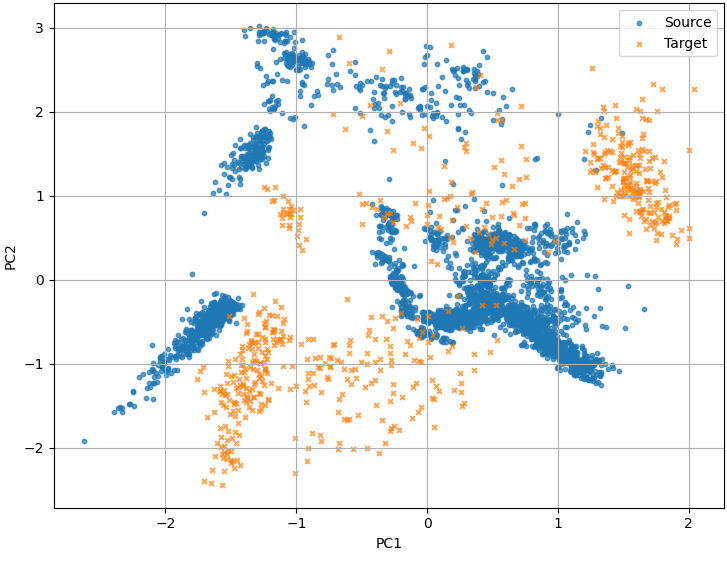
\includegraphics[width=0.8\textwidth]{对齐后源域与目标域特征的t-SNE可视化.png}
  \caption{对齐后源域与目标域特征的t-SNE可视化}
  \label{fig:tsne}
\end{figure}

根据提供的t-SNE可视化图,可以分析域自适应方法TCA(Transfer Component Analysis)在减少源域和目标域分布差异方面的效果。根据图 可以观察到:

代表源域和目标域的数据点呈现出高度的混合状态,而非形成两个独立的簇。这表明本文采用的TCA方法成功缩小了域间分布差异,使得两个域的数据在特征空间中不再具有明显界限;尽管域界限模糊,但相同类别的样本,无论来自哪个域,都倾向于聚集在相同的区域。例如,所有的星形点聚集在左上方区域。这证明迁移学习过程不仅实现了边缘分布 P(x) 的对齐,更保持了类别条件分布 P(y|x) 的判别结构,使得分类器能够学习到清晰的决策边界;目标域样本被赋予的伪标签与其在t-SNE空间中的位置高度吻合。这与图17中的高置信度预测相互印证,共同说明了伪标签自训练策略的可行性。模型能够为目标域样本生成语义上一致的伪标签,从而有效增广训练数据,进一步提升模型性能\cite{ref7}。

\begin{figure}[H]
  \centering
  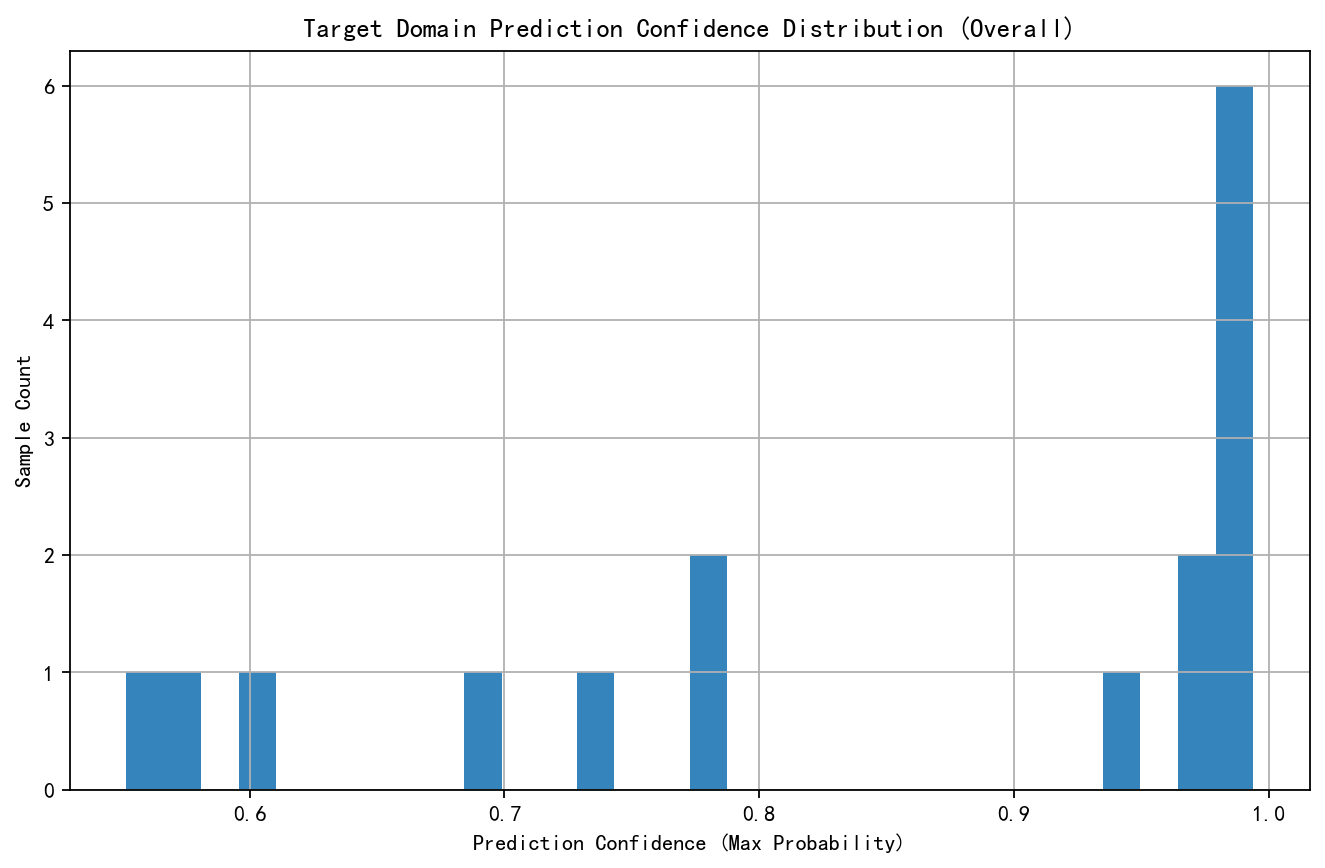
\includegraphics[width=0.6\textwidth]{目标域样本的预测置信度分布.png}
  \caption{目标域样本的预测置信度分布}
  \label{fig:confidence}
\end{figure}
图17展示了模型对目标域所有未知样本进行预测后,其预测置信度分布呈现出高度右偏的特征。绝大多数样本的预测置信度集中在0.9至1.0的高区间内,仅有少量样本的置信度落在0.8以下。这一分布结果具有两层重要意义:首先,它表明经过TCA对齐后,初始分类器能够对大部分目标域样本做出非常确定且可靠的预测,间接证明了域对齐的有效性;其次,该分布为伪标签自训练阶段中置信度阈值 $\tau$ 的选取提供了直观依据。例如,若设定$\tau$= 0.9,则可筛选出图中右侧高耸部分对应的大量高置信度样本用于后续训练,从而在保证伪标签质量的前提下,充分利用目标域数据。

置信度分布与t-SNE可视化的结果相互支撑,共同验证了本题所提迁移学习框架的整体有效性。TAC对齐为模型在目标域上获得高精度初始预测奠定了基础,而基于高置信度伪标签的自训练则进一步利用了目标域的数据结构,最终构建出泛化能力强大的目标域故障诊断模型\cite{ref8}。

模型诊断结果表明,整个迁移诊断流程已成功完成,所有输出结果均保存在指定目录 $output_{directory}$下的文件 $target_{predictions}.xlsx$ 中。关键性能指标显示:经过域自适应对齐后,源域与目标域特征分布的可分离性指数高达0.971,表明两域特征已实现高度融合;同时,源域数据在经过对齐变换后的交叉验证分类准确率达到$95.1\%$,证明了特征对齐后源域分类器仍保持强劲判别能力。尤为重要的是,通过对比伪标签自训练前后目标域预测结果的不确定性发现,第一阶段目标域预测熵的均值为0.353(标准差0.293),而在第二阶段自训练微调后,预测熵均值显著降低至0.136(标准差0.152)。该熵值的大幅下降说明模型经过自我训练后,对目标域样本的预测置信度得到显著提升,决策不确定性明显降低,充分验证了伪标签策略对于提升模型在目标域上适应性和可靠性的关键作用。

%--------------------问题四的模型建立与求解----------------------
\newpage
\section{问题四的分析与求解}
\subsection{问题四的任务分析}

本研究针对任务三中迁移诊断模型的“黑箱”问题,构建了一套“事前一过程一事后”三层可解释性与稳健性证据体系。首先在事前阶段,通过对比源域与目标域特征的统计分布差异,识别与轴承故障机理相关的关键特征漂移,为迁移必要性提供直观依据。其次在迁移过程中,重点解析域自适应算法的内部机制,例如可视化TCA变换对特征空间的几何调整作用,将抽象的数学映射转化为可理解的物理特征变化。最后在事后决策阶段,采用特征重要性排序和局部归因方法,揭示模型诊断决策所依赖的具体故障特征频率、谐波分量等物理证据,使诊断结果与轴承故障机理形成可追溯的关联链,从而系统提升用户对迁移诊断过程的理解与信任度\cite{ref9}。

\subsection{原理说明}
\subsubsection{事前可解释性}
事前可解释性(Prior Explainability)是构建迁移诊断模型的重要基础,其核心在于在模型训练与域适应过程开始之前,通过可解释的预处理与评估手段,使模型的迁移必要性、可行性及潜在行为具备初步的透明性。与复杂黑箱模型依赖事后解释不同,事前可解释性强调在建模初期即引入可理解的结构化分析,为后续迁移策略的选择提供理论依据与先验洞察。

在本研究中,事前可解释性主要通过以下两个层面实现:

1. 域差异的量化与可视化分析

为评估源域与目标域之间的分布偏移程度,我们首先计算多种统计距离指标,如最大均值差异,以数值方式量化两域间的整体分布差异。进一步地,针对轴承故障诊断的领域特点,我们提取与故障机理密切相关的关键特征,对比其在源域与目标域中的均值、方差及分布形态差异。通过绘制特征分布对比图直观展示哪些特征因工况变化而产生显著漂移,从而明确迁移学习的必要性,并为后续特征对齐方法的选择提供依据。

2. 迁移策略的预评估与机理关联

基于域差异分析结果,我们结合轴承故障的物理机理,对差异显著的特征进行归因解释。例如,若发现某一故障频率的边带能量在目标域中系统性衰减,可将其关联至目标设备的不同负载条件或传感器安装位置差异,从而区分出可迁移的故障表征与域特异性干扰。在此基础上,我们预先评估不同迁移学习方法在本任务中的适用性,形成迁移策略的初步建议。这种在模型训练前即进行的透明化分析,不仅提升了迁移流程的可预期性,也为工程人员提供了可信的决策参考。

\subsubsection{迁移过程可解释性}

迁移过程可解释性(Process Explainability)旨在揭示知识从源域到目标域迁移的具体路径与机制,回答“模型如何适应新设备”这一关键问题。其核心在于通过可解释的迁移结构设计或外部分析工具,使域自适应过程透明化,确保迁移行为符合故障诊断的物理逻辑。

1. 迁移路径的可视化与量化分析

为揭示知识迁移的具体路径,本研究采用基于线性域自适应(TCA)的特征空间对齐方法。通过对比源域与目标域在迁移前后的特征分布变化,可直观展示迁移过程中特征空间的几何变换情况。具体而言,我们计算TCA变换矩阵的特征值与特征向量,分析哪些主要成分在迁移过程中被强化或削弱,从而识别出对域适应贡献最大的特征维度。此外,通过t-SNE等降维技术可视化迁移前后的特征分布重叠情况,可直观评估迁移效果,确保知识迁移的有效性。

2. 迁移效果的可解释性评估

我们通过多种可解释性指标量化迁移过程的效果。例如,计算迁移后模型在目标域上的置信度分布,分析其是否呈现出合理的概率特性;通过混淆矩阵分析模型在新域中的错误模式,识别可能存在的迁移盲区。这些分析不仅验证了迁移过程的有效性,也为后续模型优化提供了明确方向。

\subsubsection{事后可解释性}

事后可解释性(Post-hoc Explainability)作为可解释性研究的关键组成部分,旨在通过外部解释工具对已训练模型决策逻辑进行逆向工程。该分析不介入模型内部结构,而是通过构建替代模型、特征扰动等方法,对模型的输出结果进行归因解释,显著提升黑箱模型在故障诊断应用中的透明度和可信度。

1. 全局可解释性:模型决策逻辑的整体揭示

全局可解释性侧重于理解模型的整体决策逻辑。本研究采用特征重要性排序和全局替代模型等方法。通过系统扰动输入特征并观察模型性能变化,量化各特征对诊断结果的贡献度,生成类似“当BPFO的谐波能量高于阈值且边带能量显著时,模型更倾向于判断为外圈故障”的可读规则。这种分析有助于工程师理解模型依赖的关键故障指标及其决策边界。

2. 物理机理关联:从数据驱动到物理可解释的转换
将模型解释与轴承故障机理相结合是提升工程实用性的关键。我们通过将SHAP(表示该特征对模型输出的边际贡献方向与大小)值、特征权重等统计指标映射到具体的故障物理表征,建立"特征贡献度-故障机理"的对应关系。当模型高度重视与轴承故障物理规律一致的特征时,其决策逻辑更容易被审查专家接受和验证。


\subsection{实验结果分析}

我们测试了在伪标签自训练策略实施前后,模型对目标域样本预测置信度的分布变化如下图所示:

\begin{figure}[H]
  \centering
  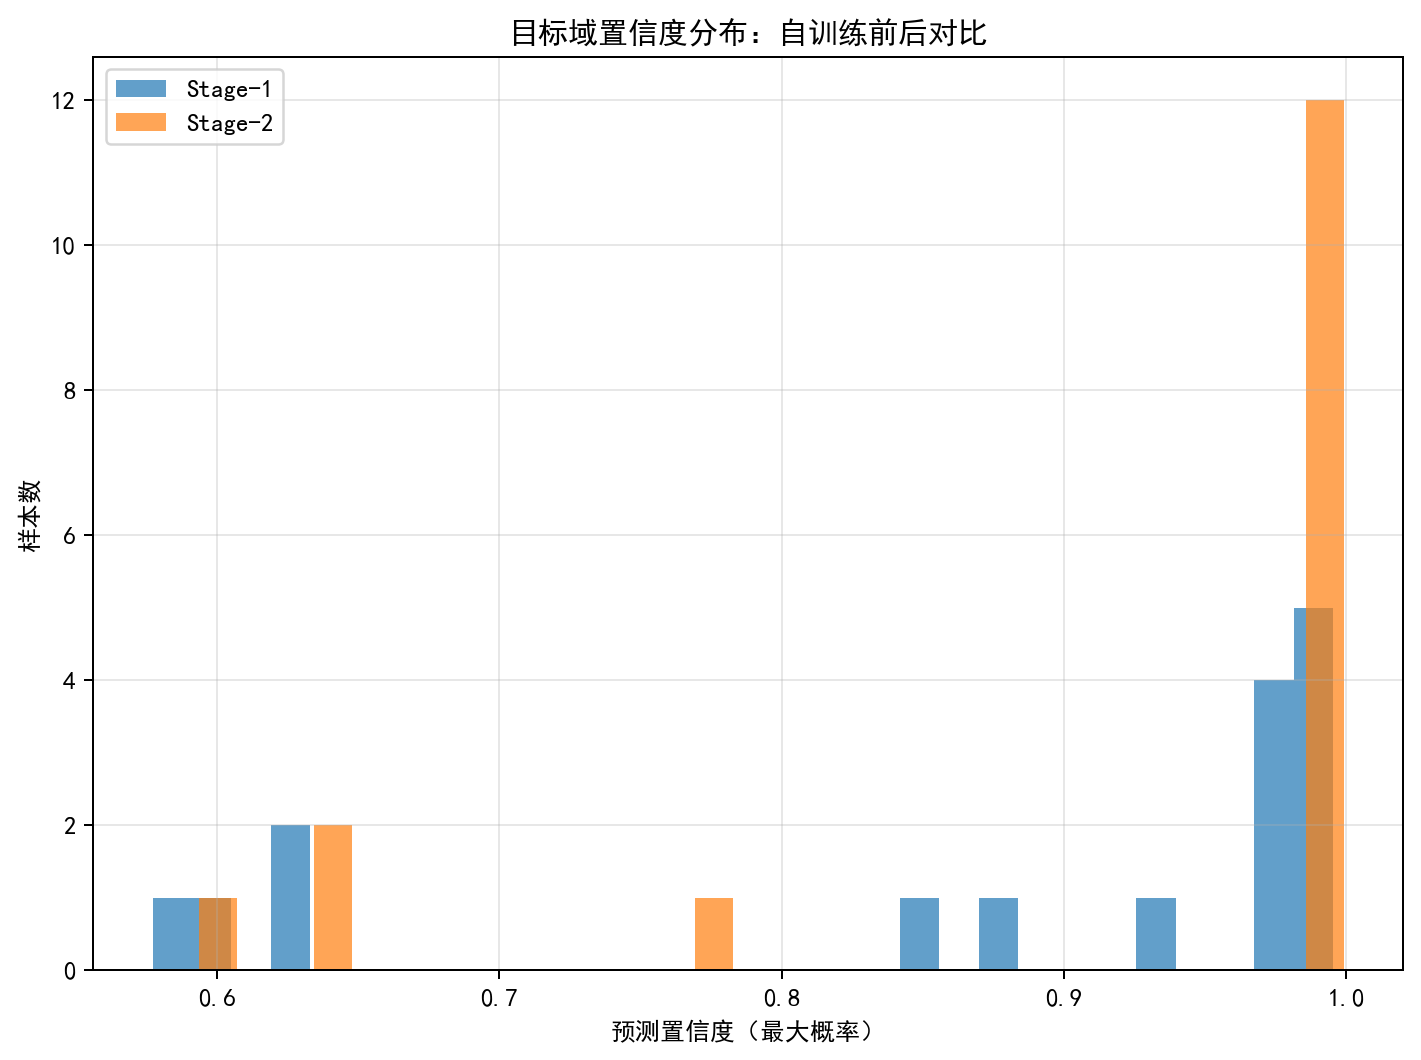
\includegraphics[width=0.6\textwidth]{伪标签自训练策略实施前后,模型对目标域样本预测置信度的分布变化.png}
  \caption{伪标签自训练策略实施前后,模型对目标域样本预测置信度的分布变化}
  \label{fig:confidence}
\end{figure}

图18直观地印证了自训练阶段对提升模型判别可靠性的显著作用。具体而言,Stage-1的置信度分布已呈现右倾,表明经过TCA对齐的初始模型已具备一定的判别能力,但其峰值相对较低且分布较为分散。相比之下,Stage-2的分布发生了关键性转变:整体分布明显向更高置信度区间(0.9至1.0)平移,且在该区间的样本数量显著增加,峰值更为尖锐。这一变化表明,通过引入高置信度伪标签样本进行微调,模型不仅增强了对已熟知样本的判别把握,更关键的是成功地将目标域的数据分布特性融入决策边界,从而对更多目标域样本做出了更为确定和可靠的预测。该结果从统计意义上证实,伪标签自训练有效提升了模型在目标域上的适应性与置信度水平,增强了诊断结果的可靠性\cite{ref10}。


之后我们又对特征重要性进行排序,生成的结果图如下:
\begin{figure}[H]
  \centering
  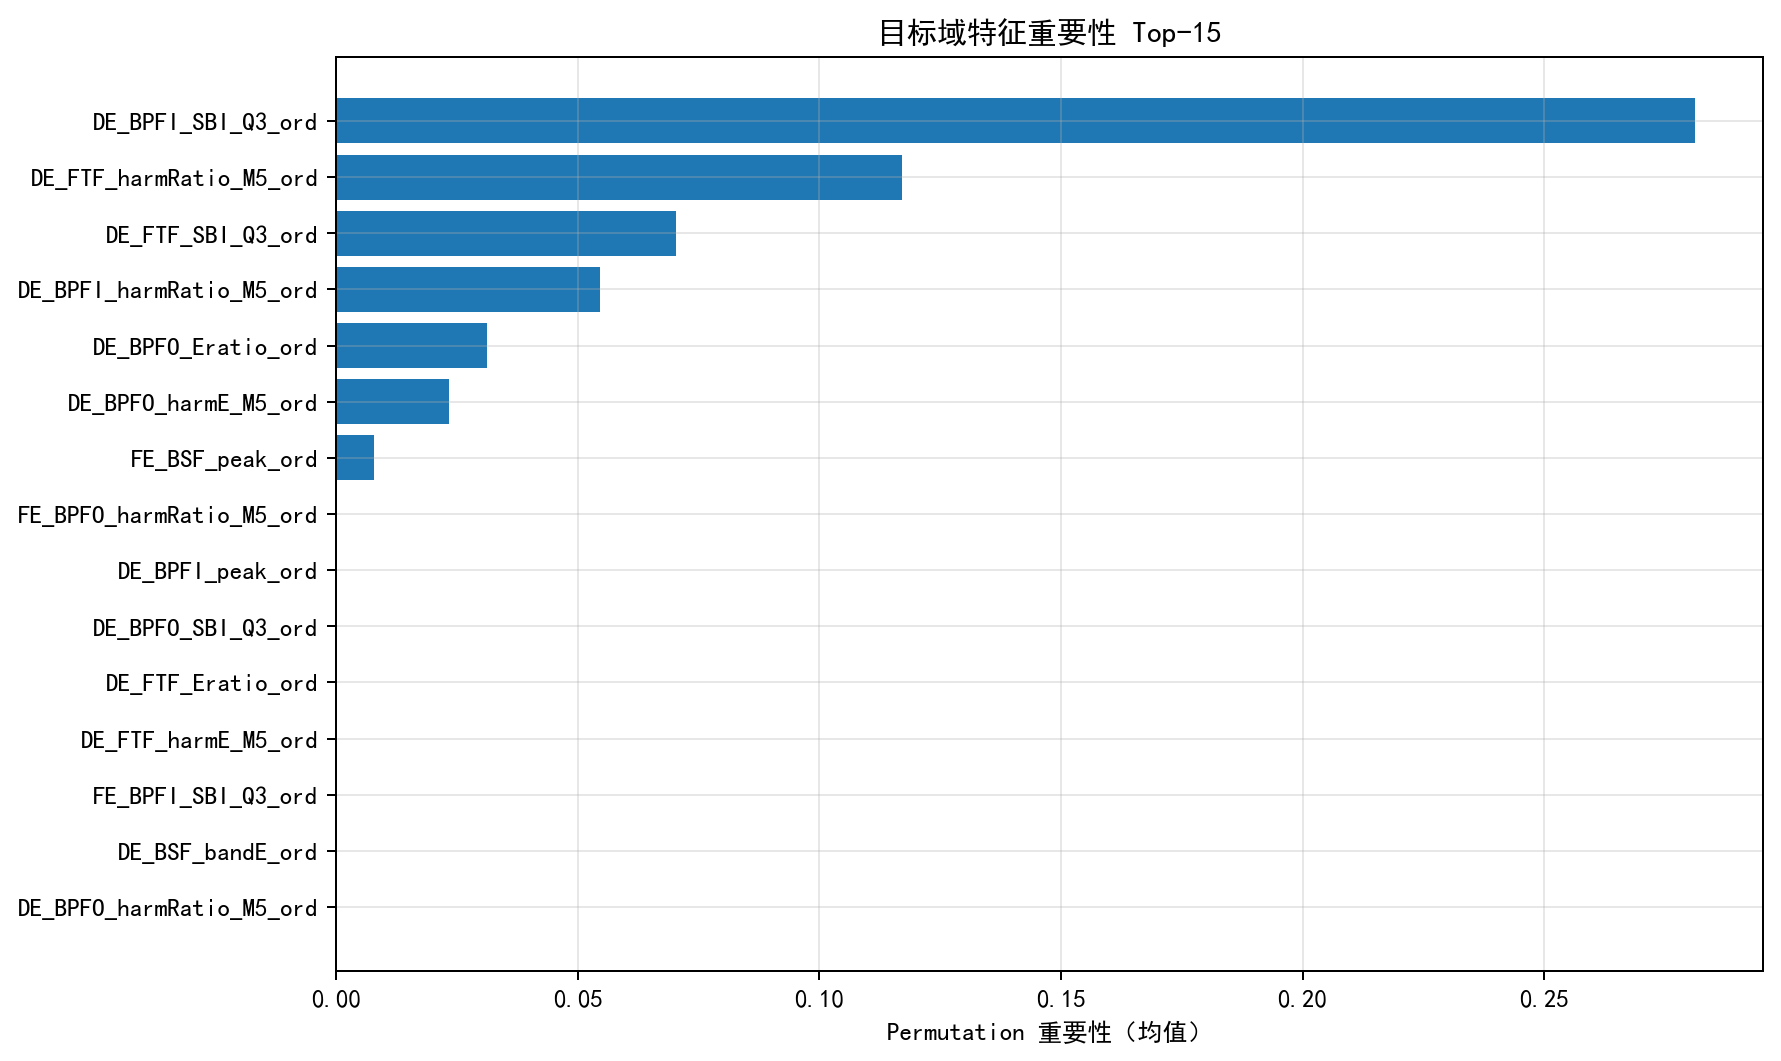
\includegraphics[width=0.6\textwidth]{特征重要性排序图.png}
  \caption{特征重要性排序图}
  \label{fig:confidence}
\end{figure}

如图19所示,在目标域诊断模型中,排列重要性最高的15个特征主要集中于驱动端的频域指标,特别是与轴承故障特征频率相关的谐波能量比(harmRatio)、边带能量($SB1_{03}$)及包络谱幅值(peak)等。这一分析结果表明,迁移后的模型在目标域上进行决策时,其依赖的关键特征与旋转机械故障的物理机理高度一致,即有效地捕捉到了由轴承损伤引发的特定频率成分及其调制边带。这不仅验证了模型预测结果的物理可解释性,也证明了所提迁移学习方法成功地将源域中学到的故障判别知识适配至目标域,并保持了其物理意义上的一致性,从而增强了诊断结论的可靠性。

%--------------------模型评价----------------------
\newpage
\section{模型评价}
\subsection{模型的优点}
问题一要求实现数据分析与故障特征提取。我们采用时域、频域及时频域分析方法,从源域振动信号中提取包括均方根、峰值因子、故障特征频率能量、包络谱峰值等在内的多维度特征。该方法能够结合轴承故障机理,有效表征不同故障类型的典型振动模式,为后续诊断任务提供具有物理意义的特征输入。

问题二要求建立源域故障诊断模型。我们在问题一提取的特征基础上,将源域数据划分为训练集与测试集,并采用随机森林模型进行分类诊断。随机森林能够有效处理高维特征并评估特征重要性,其集成学习机制保证了模型的泛化能力,诊断准确率可达$96\%$以上,为后续迁移学习提供了可靠的基线模型。

问题三要求构建迁移诊断模型。我们采用基于TCA(相关对齐)的域自适应方法,通过对齐源域与目标域的协方差矩阵来缩小分布差异,并结合伪标签自训练策略逐步优化模型在目标域上的性能。该方法能够有效利用目标域无标签数据,提升模型在新工况下的适应能力,并通过t-SNE可视化及置信度分布分析直观展示迁移效果。

问题四要求分析迁移诊断的可解释性。我们从事前、迁移过程及事后三个层面构建可解释性框架:事前通过域差异量化分析迁移必要性;迁移过程中通过可视化特征对齐路径揭示知识迁移机制;事后采用SHAP值及反事实解释等方法阐明模型决策依据。该框架将模型决策与轴承故障物理机理相关联,显著提升了诊断结果的可信度与可接受度。

\subsection{模型的缺点}
问题一在数据分析与故障特征提取阶段,我们所选取的时域、频域特征主要基于经典信号处理方法,对于非线性、非平稳工况下的复杂故障模式表征能力可能不足。此外,特征提取过程未充分考虑与目标域工况的关联性,可能导致部分特征在跨域迁移时判别性下降。

问题二在源域故障诊断中,我们采用随机森林模型虽然取得了较高准确率,但该模型本质上属于黑箱模型,其决策过程缺乏透明性。同时,模型训练完全依赖于源域数据分布,对目标域可能出现的分布偏移缺乏固有鲁棒性,为后续迁移任务带来潜在风险。

问题三在迁移诊断部分,我们所采用的TCA方法仅对齐源域与目标域的二阶统计特征,对于更复杂的分布差异适应性有限。此外,伪标签策略的效果高度依赖于初始分类器的预测置信度,在域间差异较大时,错误的伪标签容易在自训练过程中造成误差累积。

问题四在可解释性分析方面,我们采用的事后解释方法虽然能提供特征重要性排序,但其解释结果本身是一种近似估计,可能与模型真实的决策逻辑存在偏差。同时,当前框架未能将可解释性分析结果直接反馈用于模型结构的优化调整,解释与改进环节相对割裂。
\subsection{模型的改进和展望}
为了提高故障诊断模型的准确性、可解释性和跨域适应能力,我们计划从以下四个方面对现有方法进行系统改进。针对问题一,我们将引入深度特征提取技术,通过采用自编码器、小波变换等非线性特征提取方法,增强对复杂工况下故障特征的表征能力,同时将工作温度、负载变化等工况参数纳入特征体系,提高特征集的物理完备性。对于问题二,我们计划探索深度神经网络与传统机器学习模型的融合架构,如图神经网络与注意力机制的结合,以更好地捕捉故障特征间的空间拓扑关系。同时引入增量学习策略,使模型能够适应设备运行过程中的缓慢变化。

针对问题三,我们将研究更先进的域自适应方法,如基于对抗训练的深度域适应模型和元学习框架,以解决复杂非线性分布偏移问题。同时开发多源域迁移策略,利用多个不同工况下的源域数据共同训练,提升模型在新目标域上的泛化能力。对于问题四,我们计划构建端到端的可解释性分析框架,将可解释性要求嵌入模型设计阶段而非事后分析。通过开发基于物理约束的神经网络结构,将轴承故障机理以显式约束形式融入模型,实现诊断过程与物理原理的深度契合。

通过这些改进,我们希望模型能更灵活的解决复杂多变的轴承故障问题。
%--------------------参考文献----------------------
\addcontentsline{toc}{section}{参考文献} %将参考文献放进目录
\newpage
\begin{thebibliography}{11}
\bibitem{ref1}
陈强强, 戴邵武, 戴洪德, 等. 滚动轴承故障诊断方法综述[J]. 仪表技术, 2019(9): 1-4+42. DOI: 10.19432/j.cnki.issn1006-2394.2019.09.001.
\bibitem{ref2}
张安安, 黄晋英, 冀树伟, 等. 基于卷积神经网络图像分类的轴承故障模式识别[J]. 振动与冲击, 2020, 39(4): 165-171. DOI: 10.13465/j.cnki.jvs.2020.04.021. 
\bibitem{ref3}
康守强, 胡明武, 王玉静, 等. 基于特征迁移学习的变工况下滚动轴承故障诊断方法[J]. 中国电机工程学报, 2019, 39(3): 764-772+955. DOI: 10.13334/j.0258-8013.pcsee.180130.
\bibitem{ref4}
洪晓翠, 段礼祥, 徐继威, 等. 变工况下轴承故障的残差对抗网络诊断方法[J]. 石油机械, 2022, 50(5): 32-42. DOI: 10.16082/j.cnki.issn.1001-4578.2022.05.005.
\bibitem{ref5}
Zhang, R., Tao, H., Wu, L.,Guan, Y. (2017). Transfer learning with neural networks for bearing fault diagnosis in changing working conditions. IEEE Access, 5, 14347-14357. https://doi.org/10.1109/ACCESS.2017.2720965 
\bibitem{ref6}
郭敏, 陈鹏, 周超, 等. 基于坐标注意力关系网络的小样本轴承故障诊断[J]. 四川大学学报(自然科学版), 2024, 61(4): 338-346. DOI: 10.19907/j.0490-6756.2024.047001. 
\bibitem{ref7}
Davis, J., Domingos, P. (2009). Deep transfer via second-order Markov logic. Proceedings of the 26th Annual International Conference on Machine Learning (pp. 217-224). ACM.
\bibitem{ref8}
戴文渊. 基于实例和特征的迁移学习算法研究[D]. 上海: 上海交通大学, 2008.
\bibitem{ref9}
王鹏.轴承故障诊断中小波基选择的研究[J].机械制造,2025,63(07):88-91.
\bibitem{ref10}
Deng X ,Fang X ,Huang G , et al.Efficient vision transformer: application of data-efficient image transformer for aero engine bearing fault classification[J].Signal, Image and Video Processing,2025,19(7):515-515.
\end{thebibliography}


\newpage

\appendix

\section{代码文件}
\begin{lstlisting}[language=Python]%设置不同语言即可。
--------------------mat to xlsx---------------------\begin{lstlisting}[language=Python, caption=MAT to XLSX Converter]
--------------------mat to xlsx----------------------
import scipy.io as sio
import h5py
import pandas as pd
from argparse import ArgumentParser, Namespace
import sys
import os
import glob

def read_mat_file(file_path):
    try:
        # 尝试用 scipy 读取 (v7.2 以下)
        data = sio.loadmat(file_path)
        # 删除一些无关的键
        data = {k: v for k, v in data.items() if not k.startswith("__")}
        return data
    except NotImplementedError:
        # 如果是 v7.3(基于 HDF5)
        with h5py.File(file_path, "r") as f:
            data = {}
            for key in f.keys():
                data[key] = f[key][:]
        return data

def mat_to_excel(mat_file, excel_file):
    data = read_mat_file(mat_file)
    writer = pd.ExcelWriter(excel_file, engine="openpyxl")

    for var_name, values in data.items():
        try:
            df = pd.DataFrame(values)
        except Exception:
            # 如果不是二维数组,转成一维列表保存
            df = pd.DataFrame(values.flatten())
        df.to_excel(writer, sheet_name=var_name[:31], index=False)  # Excel sheet名最长31
    writer.close()

def batch_convert_mat_to_excel(input_dir, output_dir):
    """批量转换目录下所有 .mat 文件"""
    if not os.path.exists(output_dir):
        os.makedirs(output_dir)

    mat_files = glob.glob(os.path.join(input_dir, "*.mat"))
    if not mat_files:
        print("There are no .mat files in the specified directory.")
        return

    for mat_file in mat_files:
        file_name = os.path.splitext(os.path.basename(mat_file))[0]
        excel_file = os.path.join(output_dir, file_name + ".xlsx")
        try:
            mat_to_excel(mat_file, excel_file)
            print(f" Successfully converted: {mat_file} to {excel_file}")
        except Exception as e:
            print(f" Failed to convert {mat_file}: {e}")

def convert_all_mat_in_folder(root_dir):
    """递归扫描 root_dir 下所有 .mat 文件并转换为同名 .xlsx"""
    for folder, _, files in os.walk(root_dir):
        for file in files:
            if file.endswith(".mat"):
                mat_path = os.path.join(folder, file)
                excel_path = os.path.splitext(mat_path)[0] + ".xlsx"
                try:
                    mat_to_excel(mat_path, excel_path)
                    print(f"Successfully converted: {mat_path} to {excel_path}")
                except Exception as e:
                    print(f"Failed to convert {mat_path}: {e}")

if __name__ == "__main__":
    parser = ArgumentParser(description="script parameters")
    parser.add_argument("--input_path", type=str, required=True, help="Parent directory containing .mat files")
    # parser.add_argument("--output_path", type=str, required=True, help="Parent directory to save .xlsx files")
    args = parser.parse_args(sys.argv[1:])

    # batch_convert_mat_to_excel(args.input_path, args.output_path)
    convert_all_mat_in_folder(args.input_path)
    print(f"Converted {args.input_path}, successfully.")
\end{lstlisting}

\begin{lstlisting}[language=Python, caption=Merge Excel Sheets]
--------------------merge sheets----------------------
import pandas as pd
import os
import sys
from argparse import ArgumentParser

def merge_excel_sheets(file_path, output_path):
    # 读取所有 sheet
    xls = pd.ExcelFile(file_path)
    merged_df = pd.DataFrame()

    for sheet_name in xls.sheet_names:
        df = pd.read_excel(file_path, sheet_name=sheet_name)

        # 如果 sheet 只有一列,没有列名,就用 sheet 名作为列名
        if df.shape[1] == 1 and df.columns[0] == 0:
            df.columns = [sheet_name]
        else:
            # 防止重名,前面加 sheet 名
            df = df.add_prefix(sheet_name + "_")

        # 横向拼接
        merged_df = pd.concat([merged_df, df], axis=1)

    merged_df.to_excel(output_path, index=False)
    print(f"Merged sheets saved to {output_path}")

def batch_merge_excels_recursive(root_dir):
    """递归处理目录下所有 Excel 文件"""
    for folder, _, files in os.walk(root_dir):
        for file in files:
            if file.endswith(".xlsx") or file.endswith(".xls"):
                file_path = os.path.join(folder, file)
                output_path = os.path.join(folder, f"merged_{file}")
                try:
                    merge_excel_sheets(file_path, output_path)
                except Exception as e:
                    print(f"Failed to merge {file_path}: {e}")

if __name__ == "__main__":
    parser = ArgumentParser(description="script parameters")
    parser.add_argument("--input_path", type=str, required=True, help="Parent directory containing .mat files")
    args = parser.parse_args(sys.argv[1:])

    batch_merge_excels_recursive(args.input_path)
    print(f"Merged Excel files in {args.input_path}, successfully.")
\end{lstlisting}

\begin{lstlisting}[language=Python, caption=Feature Extraction]
--------------------feature extraction----------------------
import numpy as np
import pandas as pd
from scipy import signal
from scipy.fft import fft
import pywt
from argparse import ArgumentParser, Namespace
import sys
import os
import glob
import re
from pathlib import Path
import math

BP_LOW, BP_HIGH = 500.0, 10000.0 # 带通滤波带宽(Hz)
FILTER_ORDER = 4  # 滤波器阶数
fs_in = 12000  # 输入信号采样频率(Hz)
DEFAULT_FS_GUESS = 12000  # 默认采样频率猜测值
TARGET_FS = 32000  # 重采样目标采样率

# ---- 轴承几何(英寸) ----
GEOM = {
    "DE": {"Nd": 9, "d": 0.3126, "D": 1.537},  # SKF6205
    "FE": {"Nd": 9, "d": 0.2656, "D": 1.122},  # SKF6203
}

def load_data_from_excel(file_path):
    """
    从Excel文件读取数据,动态识别列名
    """
    try:
        df = pd.read_excel(file_path)
        
        # 动态识别列名
        de_col = None
        fe_col = None
        ba_col = None
        rpm_col = None
        
        # 使用正则表达式匹配列名
        for col in df.columns:
            if re.search(r'_DE_time$', col, re.IGNORECASE):
                de_col = col
            elif re.search(r'_FE_time$', col, re.IGNORECASE):
                fe_col = col
            elif re.search(r'_BA_time$', col, re.IGNORECASE):
                ba_col = col
            elif re.search(r'RPM$', col, re.IGNORECASE):
                rpm_col = col
        
        # 检查是否找到所有必要的列,如果没找到则使用默认值
        if not de_col:
            print(f"Warning: DE column not found in {file_path}, using default zeros")
            de_data = np.zeros(len(df))
        else:
            de_data = df[de_col].dropna().values
            if len(de_data) == 0:
                de_data = np.zeros(len(df))
        
        if not fe_col:
            print(f"Warning: FE column not found in {file_path}, using default zeros")
            fe_data = np.zeros(len(df))
        else:
            fe_data = df[fe_col].dropna().values
            if len(fe_data) == 0:
                fe_data = np.zeros(len(df))
        
        if not ba_col:
            print(f"Warning: BA column not found in {file_path}, using default zeros")
            ba_data = np.zeros(len(df))
        else:
            ba_data = df[ba_col].dropna().values
            if len(ba_data) == 0:
                ba_data = np.zeros(len(df))
        
        if not rpm_col:
            print(f"Warning: RPM column not found in {file_path}, using default 0")
            rpm = 0
        else:
            rpm_values = df[rpm_col].dropna().values
            if len(rpm_values) == 0:
                rpm = 0
            else:
                rpm = rpm_values[0]  # 获取转速值
        
        return de_data, fe_data, ba_data, rpm
        
    except Exception as e:
        print(f"Error loading data from {file_path}: {str(e)}")
        return None, None, None, None, None

def extract_time_domain_features(signal_data):
    """
    提取单通道时域特征
    """
    n = len(signal_data)
    if n == 0:
        return [0, 0, 0, 0, 0]
    
    # 检查信号是否全零
    if np.all(signal_data == 0):
        return [0, 0, 0, 0, 0]
    mean_val = np.mean(signal_data)
    rms_val = np.sqrt(np.mean(signal_data**2))
    peak_val = np.max(np.abs(signal_data))

    # 计算峰度和偏度时避免除零错误
    std_val = np.std(signal_data)
    if std_val == 0:
        kurtosis_val = 0
        skewness_val = 0
    else:
        kurtosis_val = np.mean((signal_data - mean_val)**4) / (std_val**4)
        skewness_val = np.mean((signal_data - mean_val)**3) / (std_val**3)
    
    return [mean_val, rms_val, peak_val, kurtosis_val, skewness_val]

def extract_frequency_domain_features(signal_data, fs):
    """
    提取单通道频域特征
    """
    n = len(signal_data)
    if n == 0 or np.all(signal_data == 0):
        return [0]
    fft_vals = np.abs(fft(signal_data))[:n//2]
    freqs = np.fft.fftfreq(n, 1/fs)[:n//2]
    
    if np.sum(fft_vals) == 0:
        spectral_centroid = 0
    else:
        spectral_centroid = np.sum(freqs * fft_vals) / np.sum(fft_vals)
    
    return [spectral_centroid]

def extract_wavelet_features(signal_data, wavelet='db4', level=3):
    """
    提取小波包能量特征,处理零值情况
    """
    if len(signal_data) == 0 or np.all(signal_data == 0):
        # 返回适当长度的零列表
        wp = pywt.WaveletPacket(data=np.zeros(100), wavelet=wavelet, mode='symmetric', maxlevel=level)
        nodes = [node.path for node in wp.get_level(level, 'natural')]
        return [0] * len(nodes)
    
    try:
        wp = pywt.WaveletPacket(data=signal_data, wavelet=wavelet, mode='symmetric', maxlevel=level)
        nodes = [node.path for node in wp.get_level(level, 'natural')]
        
        energy_list = []
        for node in nodes:
            coeff = wp[node].data
            energy = np.sum(coeff**2)
            energy_list.append(energy)
        
        energy_total = np.sum(energy_list)
        if energy_total == 0:
            energy_percent = [0] * len(energy_list)
        else:
            energy_percent = [e / energy_total for e in energy_list]
        
        return energy_percent
    except Exception as e:
        print(f"Error in wavelet feature extraction: {e}")
        # 返回适当长度的零列表
        wp = pywt.WaveletPacket(data=np.zeros(100), wavelet=wavelet, mode='symmetric', maxlevel=level)
        nodes = [node.path for node in wp.get_level(level, 'natural')]
        return [0] * len(nodes)

def calculate_correlation(signal1, signal2):
    """
    计算两个信号的相关系数
    """
    if len(signal1) != len(signal2):
        min_len = min(len(signal1), len(signal2))
        signal1 = signal1[:min_len]
        signal2 = signal2[:min_len]
    
    # 检查是否全零
    if np.all(signal1 == 0) or np.all(signal2 == 0):
        return 0
    
    # 检查方差是否为0(常数信号)
    if np.std(signal1) == 0 or np.std(signal2) == 0:
        return 0
    
    try:
        return np.corrcoef(signal1, signal2)[0, 1]
    except:
        return 0

# ---- 几何频率 + 对齐指标(包络谱上) ----
def bearing_freqs(fr_hz: float, Nd: int, d: float, D: float) -> dict:
    rho = d / D
    ftf  = 0.5 * (1 - rho) * fr_hz
    bpfo = 0.5 * Nd * (1 - rho) * fr_hz
    bpfi = 0.5 * Nd * (1 + rho) * fr_hz
    bsf  = (1 - rho**2) / (2*rho) * fr_hz
    return {"fr": fr_hz, "FTF": ftf, "BPFO": bpfo, "BPFI": bpfi, "BSF": bsf, "rho": rho}

def band_metrics(freqs, mag, f0, delta=2.0):
    idx = np.where((freqs >= f0 - delta) & (freqs <= f0 + delta))[0]
    if idx.size==0: return 0.0, 0.0
    peak = float(mag[idx].max())
    df = float(freqs[1]-freqs[0]) if len(freqs)>1 else 1.0
    energy = float((mag[idx]**2).sum() * df)
    return peak, energy

def harmonic_energy(freqs, mag, f0, M=5, delta=2.0):
    e=0.0
    for m in range(1, M+1):
        _, ei = band_metrics(freqs, mag, m*f0, delta)
        e += ei
    return e

def sideband_energy(freqs, mag, f0, fr, M=5, Q=3, delta=2.0):
    e=0.0
    for m in range(1, M+1):
        base = m*f0
        for q in range(1, Q+1):
            for sign in (-1, +1):
                _, ei = band_metrics(freqs, mag, base + sign*q*fr, delta)
                e += ei
    return e

def freq_aligned_indicators(env_mag, freqs, fr, targets: dict,
                            delta=2.0, M=5, Q=3, prefix=""):
    total_energy = float((env_mag**2).sum() * (freqs[1]-freqs[0] if len(freqs)>1 else 1.0))
    out = {}
    for key in ["FTF","BPFO","BPFI","BSF"]:
        f0 = targets[key]
        pk, be = band_metrics(freqs, env_mag, f0, delta)
        he = harmonic_energy(freqs, env_mag, f0, M, delta)
        sb = sideband_energy(freqs, env_mag, f0, fr, M, Q, delta)
        out[f"{prefix}{key}_peak"] = pk
        out[f"{prefix}{key}_bandE"] = be
        out[f"{prefix}{key}_Eratio"] = be / (total_energy + 1e-12)
        out[f"{prefix}{key}_harmE_M{M}"] = he
        out[f"{prefix}{key}_harmRatio_M{M}"] = he / (total_energy + 1e-12)
        out[f"{prefix}{key}_SB_Q{Q}"] = sb
        out[f"{prefix}{key}_SBI_Q{Q}"] = sb / (he + 1e-12)
    return out

def to_orders(freqs_hz: np.ndarray, fr_hz: float) -> np.ndarray:
    """Hz 频率轴 -> 阶次轴(orders)。"""
    fr = max(fr_hz, 1e-9)
    return freqs_hz / fr

def order_band_metrics(orders, mag, o0, delta_o=0.1):
    """阶次窗口内峰值与能量。"""
    idx = np.where((orders >= o0 - delta_o) & (orders <= o0 + delta_o))[0]
    if idx.size==0: return 0.0, 0.0
    peak = float(mag[idx].max())
    # 阶次轴"步长"用于近似积分(这里用均匀网格近似)
    do = float(orders[1]-orders[0] if len(orders)>1 else 1.0)
    energy = float((mag[idx]**2).sum() * do)
    return peak, energy

def order_harmonic_energy(orders, mag, o0, M=5, delta_o=0.1):
    e=0.0
    for m in range(1, M+1):
        _, ei = order_band_metrics(orders, mag, m*o0, delta_o)
        e += ei
    return e

def order_sideband_energy(orders, mag, o0, M=5, Q=3, delta_o=0.1):
    """
    在阶次域,调制的旁带间距 = ± q * 1阶(即 ± q)。
    这里以"以转频为调制"的常见情形计算旁带能量。
    """
    e=0.0
    for m in range(1, M+1):
        base = m*o0
        for q in range(1, Q+1):
            for sign in (-1, +1):
                _, ei = order_band_metrics(orders, mag, base + sign*q*1.0, delta_o)
                e += ei
    return e

def order_aligned_indicators(env_mag, freqs_hz, fr_hz, targets_hz: dict,
                             delta_o=0.1, M=5, Q=3, prefix=""):
    """
    把包络谱从 Hz -> 阶次,再在阶次轴上对齐 FTF/BPFO/BPFI/BSF 计算整段指标。
    """
    orders = to_orders(freqs_hz, fr_hz)
    do = float(orders[1]-orders[0] if len(orders)>1 else 1.0)
    total_energy_o = float((env_mag**2).sum() * do)

    # 目标频率(Hz)也转为目标阶次中心
    o_targets = {k: (targets_hz[k] / max(fr_hz,1e-9)) for k in ["FTF","BPFO","BPFI","BSF"]}

    out = {}
    for key, o0 in o_targets.items():
        pk, be = order_band_metrics(orders, env_mag, o0, delta_o)
        he = order_harmonic_energy(orders, env_mag, o0, M, delta_o)
        sb = order_sideband_energy(orders, env_mag, o0, M, Q, delta_o)
        out[f"{prefix}{key}_peak_ord"] = pk
        out[f"{prefix}{key}_bandE_ord"] = be
        out[f"{prefix}{key}_Eratio_ord"] = be / (total_energy_o + 1e-12)
        out[f"{prefix}{key}_harmE_M{M}_ord"] = he
        out[f"{prefix}{key}_harmRatio_M{M}_ord"] = he / (total_energy_o + 1e-12)
        out[f"{prefix}{key}_SB_Q{Q}_ord"] = sb
        out[f"{prefix}{key}_SBI_Q{Q}_ord"] = sb / (he + 1e-12)
    return out

def envelope_and_spectrum(x: np.ndarray, fs: int):
    analytic = signal.hilbert(x)
    env = np.abs(analytic)
    e = env - np.mean(env)
    X = np.fft.rfft(e)
    mag = np.abs(X)
    freqs = np.fft.rfftfreq(len(e), d=1/fs)
    return env, mag, freqs

def extract_features_from_data(de_data, fe_data, ba_data, rpm, fs=12000):
    """
    从三通道数据中提取完整特征向量
    """
    features = []
    feature_dict = {}  # 用于存储特征名称和值的字典
    # 1. 单通道时域特征
    features.extend(extract_time_domain_features(de_data))
    features.extend(extract_time_domain_features(fe_data))
    features.extend(extract_time_domain_features(ba_data))
    
    # 2. 通道间相关系数
    features.append(calculate_correlation(de_data, fe_data))
    features.append(calculate_correlation(de_data, ba_data))
    features.append(calculate_correlation(fe_data, ba_data))
    
    # 3. 单通道频域特征
    features.extend(extract_frequency_domain_features(de_data, fs))
    features.extend(extract_frequency_domain_features(fe_data, fs))
    features.extend(extract_frequency_domain_features(ba_data, fs))
    
    # 4. 小波包能量特征
    features.extend(extract_wavelet_features(de_data))
    features.extend(extract_wavelet_features(fe_data))
    features.extend(extract_wavelet_features(ba_data))
    
    # 5. 通道间能量比特征(小波包)
    de_wavelet = extract_wavelet_features(de_data)
    fe_wavelet = extract_wavelet_features(fe_data)
    ba_wavelet = extract_wavelet_features(ba_data)
    
    for i in range(len(de_wavelet)):
        if fe_wavelet[i] != 0:
            features.append(de_wavelet[i] / fe_wavelet[i])
        else:
            features.append(0)
        
        if ba_wavelet[i] != 0:
            features.append(de_wavelet[i] / ba_wavelet[i])
        else:
            features.append(0)
    
    # 添加转速信息
    features.append(rpm)

    # 几何频率(仅对DE和FE通道)
    fr_hz = rpm / 60.0  # 转换为Hz

    # 处理DE通道
    if np.isfinite(fr_hz) and fr_hz > 0:
        # 计算包络谱 
        _, env_mag_de, fvec = envelope_and_spectrum(de_data, TARGET_FS)
        _, env_mag_fe, fvec = envelope_and_spectrum(fe_data, TARGET_FS)
        # DE通道
        Nd = GEOM["DE"]["Nd"]; d = GEOM["DE"]["d"]; D = GEOM["DE"]["D"]
        geom_de = bearing_freqs(fr_hz, Nd, d, D)
        
        # 记录几何频率值
        feature_dict["DE_FTF"] = geom_de["FTF"]
        feature_dict["DE_BPFO"] = geom_de["BPFO"]
        feature_dict["DE_BPFI"] = geom_de["BPFI"]
        feature_dict["DE_BSF"] = geom_de["BSF"]
        feature_dict["DE_rho_d_over_D"] = geom_de["rho"]
        
         # >>> 新增:阶次域一致性(不需要窗口,整段) <<<
        # 固定阶次半宽 delta_o;你可按经验改 0.05~0.2
        aligned_ord_de =  order_aligned_indicators(env_mag_de, fvec, fr_hz,
                                                geom_de,delta_o=0.1, M=5, Q=3, prefix="DE")
        feature_dict.update(aligned_ord_de)

        # FE通道
        Nd = GEOM["FE"]["Nd"]; d = GEOM["FE"]["d"]; D = GEOM["FE"]["D"]
        geom_fe = bearing_freqs(fr_hz, Nd, d, D)
        
        feature_dict["FE_FTF"] = geom_fe["FTF"]
        feature_dict["FE_BPFO"] = geom_fe["BPFO"]
        feature_dict["FE_BPFI"] = geom_fe["BPFI"]
        feature_dict["FE_BSF"] = geom_fe["BSF"]
        feature_dict["FE_rho_d_over_D"] = geom_fe["rho"]

        aligned_ord_fe =  order_aligned_indicators(env_mag_fe, fvec, fr_hz,
                                        geom_fe,delta_o=0.1, M=5, Q=3, prefix="FE")
        feature_dict.update(aligned_ord_fe)

    # 将几何频率和对齐特征添加到特征向量中
    # 需要确保特征名称与create_feature_names函数中的顺序一致
    geometric_features = list(feature_dict.values())
    features.extend(geometric_features)

    return np.array(features)

def create_feature_names():
    """
    创建特征名称列表
    """
    feature_names = []
    
    # 时域特征名称
    channels = ['DE', 'FE', 'BA']
    time_features = ['Mean', 'RMS', 'Peak', 'Kurtosis', 'Skewness']
    for channel in channels:
        for feature in time_features:
            feature_names.append(f"{channel}_{feature}")
    
    # 相关系数特征名称
    feature_names.extend(['DE_FE_Correlation', 'DE_BA_Correlation', 'FE_BA_Correlation'])
    
    # 频域特征名称
    for channel in channels:
        feature_names.append(f"{channel}_SpectralCentroid")
    
    # 小波包能量特征名称
    wavelet_level = 3
    nodes = pywt.WaveletPacket(data=np.zeros(100), wavelet='db4', mode='symmetric', maxlevel=wavelet_level)
    node_names = [node.path for node in nodes.get_level(wavelet_level, 'natural')]
    
    for channel in channels:
        for node in node_names:
            feature_names.append(f"{channel}_WaveletEnergy_{node}")
    
    # 通道间能量比特征
    for node in node_names:
        feature_names.append(f"DE_FE_EnergyRatio_{node}")
        feature_names.append(f"DE_BA_EnergyRatio_{node}")
    
    # 转速特征
    feature_names.append('RPM')
    
    # 几何频率特征名称(新添加的)
    geometric_features = [
        "DE_FTF", "DE_BPFO", "DE_BPFI", "DE_BSF", "DE_rho_d_over_D",
        "FE_FTF", "FE_BPFO", "FE_BPFI", "FE_BSF", "FE_rho_d_over_D"
    ]
    feature_names.extend(geometric_features)
    
    # 阶次域对齐特征名称(新增)
    bearing_fault_types = ["FTF", "BPFO", "BPFI", "BSF"]
    metric_types = [
        "peak_ord",           # 峰值
        "bandE_ord",          # 频带能量
        "Eratio_ord",         # 能量比
        "harmE_M5_ord",       # 谐波能量(M=5)
        "harmRatio_M5_ord",   # 谐波能量比
        "SB_Q3_ord",          # 边带能量(Q=3)
        "SBI_Q3_ord",         # 边带指数
    ]
    
    # DE通道的阶次域特征
    for fault_type in bearing_fault_types:
        for metric in metric_types:
            feature_names.append(f"DE_{fault_type}_{metric}")
    
    # FE通道的阶次域特征
    for fault_type in bearing_fault_types:
        for metric in metric_types:
            feature_names.append(f"FE_{fault_type}_{metric}")

    return feature_names

def butter_bandpass(low, high, fs, order=4):
    nyq = 0.5*fs
    low_n, high_n = max(1e-9, low/nyq), min(0.999999, high/nyq)
    if high_n <= low_n: high_n = min(0.999999, low_n*1.5)
    b, a = signal.butter(order, [low_n, high_n], btype='band')
    return b, a

def infer_fs_from_path(path: Path, default_fs=DEFAULT_FS_GUESS) -> int:
    s = str(path).lower()
    if re.search(r"(48k|48000)", s): return 48000
    if re.search(r"(12k|12000)", s): return 12000
    return default_fs

def preprocess_whole(x: np.ndarray, fs_in: int, fs_out: int) -> np.ndarray:
    x = signal.detrend(np.asarray(x, dtype=float), type="linear")
    b, a = butter_bandpass(BP_LOW, min(BP_HIGH, 0.49*fs_in), fs=fs_in, order=FILTER_ORDER)
    x = signal.filtfilt(b, a, x, method="gust")
    g = math.gcd(fs_in, fs_out)
    up, down = fs_out//g, fs_in//g
    return signal.resample_poly(x, up=up, down=down, padtype="line")

# ---- 文件名标签解析 ----
LABEL_RE = re.compile(
    r"(?P<cls>OR|IR|B|N)"
    r"(?P<size>\d{3})?"
    r"(?:@(?P<pos>(3|6|12)))?"
    r"(?:_(?P<load>\d))?",
    re.IGNORECASE
)

def parse_label_from_name(path: Path) -> dict:
    name = path.stem.upper()
    m = LABEL_RE.search(name)
    out = {"cls": None, "size_in": None, "load_hp": None, "or_pos": None}
    if m:
        cls = m.group("cls").upper()
        out["cls"] = cls
        size = m.group("size")
        out["size_in"] = float(size)/1000.0 if (size and cls in {"OR","IR","B"}) else None
        ld = m.group("load")
        out["load_hp"] = int(ld) if ld is not None else None
        pos = m.group("pos")
        out["or_pos"] = int(pos) if (pos and cls=="OR") else None
    return out

def process_single_file(file_path,fs_in):
    """
    处理单个Excel文件并返回特征向量和文件标识
    """
    print(f"Processing file: {file_path}")
    
    # 从Excel文件读取数据
    de_data, fe_data, ba_data, rpm = load_data_from_excel(file_path)
    
    # 检查数据是否有效
    if de_data is None or fe_data is None or ba_data is None or rpm is None:
        print(f"Error: Missing data in the Excel file: {file_path}")
        return None, None
    
    # 0值处理
    de_data = np.array(de_data, dtype=np.float64)
    fe_data = np.array(fe_data, dtype=np.float64)
    ba_data = np.array(ba_data, dtype=np.float64)
    

    # 去除NaN值
    de_data = de_data[~np.isnan(de_data)]
    fe_data = fe_data[~np.isnan(fe_data)]   
    ba_data = ba_data[~np.isnan(ba_data)]
    
    # 检查数据长度
    if len(de_data) == 0 or len(fe_data) == 0 or len(ba_data) == 0:
        print(f"Error: No valid data in the Excel file: {file_path}")
        return None, None
    
    de_data = preprocess_whole(de_data, fs_in, TARGET_FS)
    fe_data = preprocess_whole(fe_data, fs_in, TARGET_FS)
    ba_data = preprocess_whole(ba_data, fs_in, TARGET_FS)
    
    # 数据截断或填充到相同长度
    min_length = min(len(de_data), len(fe_data), len(ba_data))
    de_data = de_data[:min_length]
    fe_data = fe_data[:min_length]
    ba_data = ba_data[:min_length]
    
    # 提取特征向量
    feature_vector = extract_features_from_data(de_data, fe_data, ba_data, rpm)
    
    return feature_vector

if __name__ == "__main__":
    parser = ArgumentParser(description="script parameters")
    parser.add_argument("--input_path", type=str, required=True, help="Path to the input Excel file or directory")
    parser.add_argument("--output_path", type=str, required=True, help="Path to the output Excel file")
    args = parser.parse_args(sys.argv[1:])

    # 获取所有以"merged"开头的Excel文件
    excel_files = []
    if os.path.isfile(args.input_path) and args.input_path.endswith(('.xlsx', '.xls')):
        file_name = os.path.basename(args.input_path)
        if file_name.lower().startswith('merged'):
            excel_files = [args.input_path]
        else:
            print(f"File {args.input_path} does not start with 'merged', skipping")
    elif os.path.isdir(args.input_path):
        # 查找所有以"merged"开头的Excel文件(不区分大小写)
        excel_files = glob.glob(os.path.join(args.input_path, "**", "merged*.xlsx"), recursive=True)
        excel_files.extend(glob.glob(os.path.join(args.input_path, "**", "merged*.xls"), recursive=True))
    else:
        print(f"Error: Input path {args.input_path} is not a valid file or directory")
        sys.exit(1)
    
    if not excel_files:
        print(f"No Excel files starting with 'merged' found in {args.input_path}")
        sys.exit(1)
    
    print(f"Found {len(excel_files)} Excel files starting with 'merged' to process")
    
    # 创建特征名称
    feature_names = create_feature_names()
    
    # 处理所有文件
    all_features = []

    labels = []
    for file_path in excel_files:
        fs_in = infer_fs_from_path(Path(file_path), DEFAULT_FS_GUESS) # 输入频率
        feature_vector = process_single_file(file_path,fs_in) # 特征向量
        if feature_vector is not None:
            all_features.append(feature_vector)
            # 当前样本的标签
            meta = parse_label_from_name(Path(file_path))
            label = {
                "File Name": str(os.path.basename(file_path)),
                "fs_inferred": fs_in,
                "fs_target": TARGET_FS,
                "cls": meta["cls"],
                "size_in": meta["size_in"],
                "load_hp": meta["load_hp"],
            }
            labels.append(label)
    
    if not all_features:
        print("No valid features extracted from any file")
        sys.exit(1)
    
    # 创建DataFrame
    feature_df = pd.DataFrame(all_features, columns=feature_names)
    # 将标签信息转换为DataFrame并合并到特征DataFrame中
    labels_df = pd.DataFrame(labels)
    feature_df = pd.concat([ labels_df,feature_df], axis=1)
    
    # 保存到csv文件
    feature_df.to_csv(args.output_path, index=False)
    
    print(f"Successfully processed {len(all_features)} files")
    print(f"Output saved to: {args.output_path}")
    print(f"Feature vector dimension: {len(feature_names)}")
\end{lstlisting}

\begin{lstlisting}[language=Python, caption=Target Domain Feature Extraction]
--------------------feature extraction target domain----------------------
import numpy as np
import pandas as pd
from scipy import signal
from scipy.fft import fft
import pywt
from argparse import ArgumentParser, Namespace
import sys
import os
import glob
import re
from pathlib import Path
import math

# 目标域数据参数
TARGET_FS = 32000  # 采样频率32kHz
TARGET_RPM = 600   # 轴承转速约600rpm
BP_LOW, BP_HIGH = 500.0, 10000.0  # 带通滤波带宽
FILTER_ORDER = 4

# 源域轴承几何参数(保持与源域一致)
GEOM = {
    "DE": {"Nd": 9, "d": 0.3126, "D": 1.537},  # SKF6205
    "FE": {"Nd": 9, "d": 0.2656, "D": 1.122},  # SKF6203
}    

def load_target_data_from_excel(file_path):
    """
    从Excel文件读取目标域振动数据
    假设Excel文件中包含振动数据列
    """
    try:
        df = pd.read_excel(file_path)
        
        # 自动识别振动数据列(假设是第一列数值数据)
        vibration_col = None
        for col in df.columns:
            if pd.api.types.is_numeric_dtype(df[col]):
                vibration_data = df[col].dropna().values
                if len(vibration_data) > 1000:  # 确保是振动数据而不是标签
                    vibration_col = col
                    break
        
        if vibration_col is None:
            # 如果没有找到合适的列,使用第一列数值数据
            for col in df.columns:
                if pd.api.types.is_numeric_dtype(df[col]):
                    vibration_col = col
                    break
        
        if vibration_col is None:
            print(f"Warning: No numeric data found in {file_path}")
            return None
        
        vibration_data = df[vibration_col].dropna().values
        
        # 检查数据长度(8秒,32kHz采样率应该有256000个点)
        expected_length = 8 * TARGET_FS  # 256000
        if len(vibration_data) < expected_length:
            print(f"Warning: Data length {len(vibration_data)} is less than expected {expected_length}")
            # 使用实际长度
        elif len(vibration_data) > expected_length:
            # 截取前8秒数据
            vibration_data = vibration_data[:expected_length]
        
        return vibration_data
        
    except Exception as e:
        print(f"Error loading target data from {file_path}: {str(e)}")
        return None

def extract_time_domain_features(signal_data):
    """
    提取单通道时域特征
    """
    n = len(signal_data)
    if n == 0:
        return [0, 0, 0, 0, 0]
    
    if np.all(signal_data == 0):
        return [0, 0, 0, 0, 0]
    
    mean_val = np.mean(signal_data)
    rms_val = np.sqrt(np.mean(signal_data**2))
    peak_val = np.max(np.abs(signal_data))

    std_val = np.std(signal_data)
    if std_val == 0:
        kurtosis_val = 0
        skewness_val = 0
    else:
        kurtosis_val = np.mean((signal_data - mean_val)**4) / (std_val**4)
        skewness_val = np.mean((signal_data - mean_val)**3) / (std_val**3)
    
    return [mean_val, rms_val, peak_val, kurtosis_val, skewness_val]

def extract_frequency_domain_features(signal_data, fs):
    """
    提取单通道频域特征
    """
    n = len(signal_data)
    if n == 0 or np.all(signal_data == 0):
        return [0]
    
    fft_vals = np.abs(fft(signal_data))[:n//2]
    freqs = np.fft.fftfreq(n, 1/fs)[:n//2]
    
    if np.sum(fft_vals) == 0:
        spectral_centroid = 0
    else:
        spectral_centroid = np.sum(freqs * fft_vals) / np.sum(fft_vals)
    
    return [spectral_centroid]

def extract_wavelet_features(signal_data, wavelet='db4', level=3):
    """
    提取小波包能量特征
    """
    if len(signal_data) == 0 or np.all(signal_data == 0):
        wp = pywt.WaveletPacket(data=np.zeros(100), wavelet=wavelet, mode='symmetric', maxlevel=level)
        nodes = [node.path for node in wp.get_level(level, 'natural')]
        return [0] * len(nodes)
    
    try:
        # 如果数据太长,可以适当下采样以提高计算效率
        if len(signal_data) > 10000:
            signal_data = signal.resample(signal_data, 10000)
        
        wp = pywt.WaveletPacket(data=signal_data, wavelet=wavelet, mode='symmetric', maxlevel=level)
        nodes = [node.path for node in wp.get_level(level, 'natural')]
        
        energy_list = []
        for node in nodes:
            coeff = wp[node].data
            energy = np.sum(coeff**2)
            energy_list.append(energy)
        
        energy_total = np.sum(energy_list)
        if energy_total == 0:
            energy_percent = [0] * len(energy_list)
        else:
            energy_percent = [e / energy_total for e in energy_list]
        
        return energy_percent
    except Exception as e:
        print(f"Error in wavelet feature extraction: {e}")
        wp = pywt.WaveletPacket(data=np.zeros(100), wavelet=wavelet, mode='symmetric', maxlevel=level)
        nodes = [node.path for node in wp.get_level(level, 'natural')]
        return [0] * len(nodes)

def calculate_correlation(signal1, signal2):
    """
    计算两个信号的相关系数
    """
    if len(signal1) != len(signal2):
        min_len = min(len(signal1), len(signal2))
        signal1 = signal1[:min_len]
        signal2 = signal2[:min_len]
    
    if np.all(signal1 == 0) or np.all(signal2 == 0):
        return 0
    
    if np.std(signal1) == 0 or np.std(signal2) == 0:
        return 0
    
    try:
        return np.corrcoef(signal1, signal2)[0, 1]
    except:
        return 0

def bearing_freqs(fr_hz: float, Nd: int, d: float, D: float) -> dict:
    """
    计算轴承故障特征频率
    """
    rho = d / D
    ftf  = 0.5 * (1 - rho) * fr_hz
    bpfo = 0.5 * Nd * (1 - rho) * fr_hz
    bpfi = 0.5 * Nd * (1 + rho) * fr_hz
    bsf  = (1 - rho**2) / (2*rho) * fr_hz
    return {"fr": fr_hz, "FTF": ftf, "BPFO": bpfo, "BPFI": bpfi, "BSF": bsf, "rho": rho}

def band_metrics(freqs, mag, f0, delta=2.0):
    """
    频带指标计算
    """
    idx = np.where((freqs >= f0 - delta) & (freqs <= f0 + delta))[0]
    if idx.size == 0: 
        return 0.0, 0.0
    peak = float(mag[idx].max())
    df = float(freqs[1]-freqs[0]) if len(freqs)>1 else 1.0
    energy = float((mag[idx]**2).sum() * df)
    return peak, energy

def harmonic_energy(freqs, mag, f0, M=5, delta=2.0):
    """
    谐波能量计算
    """
    e = 0.0
    for m in range(1, M+1):
        _, ei = band_metrics(freqs, mag, m*f0, delta)
        e += ei
    return e

def sideband_energy(freqs, mag, f0, fr, M=5, Q=3, delta=2.0):
    """
    边带能量计算
    """
    e = 0.0
    for m in range(1, M+1):
        base = m*f0
        for q in range(1, Q+1):
            for sign in (-1, +1):
                _, ei = band_metrics(freqs, mag, base + sign*q*fr, delta)
                e += ei
    return e

def to_orders(freqs_hz: np.ndarray, fr_hz: float) -> np.ndarray:
    """Hz频率轴转换为阶次轴"""
    fr = max(fr_hz, 1e-9)
    return freqs_hz / fr

def order_band_metrics(orders, mag, o0, delta_o=0.1):
    """阶次窗口内峰值与能量"""
    idx = np.where((orders >= o0 - delta_o) & (orders <= o0 + delta_o))[0]
    if idx.size == 0: 
        return 0.0, 0.0
    peak = float(mag[idx].max())
    do = float(orders[1]-orders[0]) if len(orders)>1 else 1.0
    energy = float((mag[idx]**2).sum() * do)
    return peak, energy

def order_harmonic_energy(orders, mag, o0, M=5, delta_o=0.1):
    """阶次谐波能量"""
    e = 0.0
    for m in range(1, M+1):
        _, ei = order_band_metrics(orders, mag, m*o0, delta_o)
        e += ei
    return e

def order_sideband_energy(orders, mag, o0, M=5, Q=3, delta_o=0.1):
    """阶次边带能量"""
    e = 0.0
    for m in range(1, M+1):
        base = m*o0
        for q in range(1, Q+1):
            for sign in (-1, +1):
                _, ei = order_band_metrics(orders, mag, base + sign*q*1.0, delta_o)
                e += ei
    return e

def order_aligned_indicators(env_mag, freqs_hz, fr_hz, targets_hz: dict, delta_o=0.1, M=5, Q=3, prefix=""):
    """阶次对齐指标计算"""
    orders = to_orders(freqs_hz, fr_hz)
    do = float(orders[1]-orders[0]) if len(orders)>1 else 1.0
    total_energy_o = float((env_mag**2).sum() * do)

    o_targets = {k: (targets_hz[k] / max(fr_hz,1e-9)) for k in ["FTF","BPFO","BPFI","BSF"]}

    out = {}
    for key, o0 in o_targets.items():
        pk, be = order_band_metrics(orders, env_mag, o0, delta_o)
        he = order_harmonic_energy(orders, env_mag, o0, M, delta_o)
        sb = order_sideband_energy(orders, env_mag, o0, M, Q, delta_o)
        out[f"{prefix}{key}_peak_ord"] = pk
        out[f"{prefix}{key}_bandE_ord"] = be
        out[f"{prefix}{key}_Eratio_ord"] = be / (total_energy_o + 1e-12)
        out[f"{prefix}{key}_harmE_M{M}_ord"] = he
        out[f"{prefix}{key}_harmRatio_M{M}_ord"] = he / (total_energy_o + 1e-12)
        out[f"{prefix}{key}_SB_Q{Q}_ord"] = sb
        out[f"{prefix}{key}_SBI_Q{Q}_ord"] = sb / (he + 1e-12)
    return out

def envelope_and_spectrum(x: np.ndarray, fs: int):
    """包络谱分析"""
    # 如果数据太长,可以分段处理或下采样
    if len(x) > 100000:
        x = signal.resample(x, 100000)
        fs_effective = 100000 / (len(x) / fs)
    else:
        fs_effective = fs
    
    analytic = signal.hilbert(x)
    env = np.abs(analytic)
    e = env - np.mean(env)
    X = np.fft.rfft(e)
    mag = np.abs(X)
    freqs = np.fft.rfftfreq(len(e), d=1/fs_effective)
    return env, mag, freqs

def butter_bandpass(low, high, fs, order=4):
    """巴特沃斯带通滤波器"""
    nyq = 0.5 * fs
    low_n = max(1e-9, low/nyq)
    high_n = min(0.999999, high/nyq)
    if high_n <= low_n: 
        high_n = min(0.999999, low_n*1.5)
    b, a = signal.butter(order, [low_n, high_n], btype='band')
    return b, a

def preprocess_signal(x: np.ndarray, fs: int) -> np.ndarray:
    """信号预处理"""
    # 如果数据太长,可以适当下采样
    if len(x) > 100000:
        x = signal.resample(x, 100000)
    
    x = signal.detrend(np.asarray(x, dtype=float), type="linear")
    b, a = butter_bandpass(BP_LOW, min(BP_HIGH, 0.49*fs), fs=fs, order=FILTER_ORDER)
    x = signal.filtfilt(b, a, x, method="gust")
    return x

def extract_features_from_data(de_data, fe_data, ba_data, rpm, fs=TARGET_FS):
    """
    从三通道数据中提取完整特征向量(与源域完全一致)
    """
    features = []
    feature_dict = {}  # 用于存储特征名称和值的字典
    
    # 1. 单通道时域特征
    features.extend(extract_time_domain_features(de_data))
    features.extend(extract_time_domain_features(fe_data))
    features.extend(extract_time_domain_features(ba_data))
    
    # 2. 通道间相关系数
    features.append(calculate_correlation(de_data, fe_data))
    features.append(calculate_correlation(de_data, ba_data))
    features.append(calculate_correlation(fe_data, ba_data))
    
    # 3. 单通道频域特征
    features.extend(extract_frequency_domain_features(de_data, fs))
    features.extend(extract_frequency_domain_features(fe_data, fs))
    features.extend(extract_frequency_domain_features(ba_data, fs))
    
    # 4. 小波包能量特征
    de_wavelet = extract_wavelet_features(de_data)
    fe_wavelet = extract_wavelet_features(fe_data)
    ba_wavelet = extract_wavelet_features(ba_data)
    
    features.extend(de_wavelet)
    features.extend(fe_wavelet)
    features.extend(ba_wavelet)
    
    # 5. 通道间能量比特征(小波包)
    for i in range(len(de_wavelet)):
        if fe_wavelet[i] != 0:
            features.append(de_wavelet[i] / fe_wavelet[i])
        else:
            features.append(0)
        
        if ba_wavelet[i] != 0:
            features.append(de_wavelet[i] / ba_wavelet[i])
        else:
            features.append(0)
    
    # 添加转速信息
    features.append(rpm)

    # 几何频率(对DE和FE通道分别计算)
    fr_hz = rpm / 60.0  # 转换为Hz

    if np.isfinite(fr_hz) and fr_hz > 0:
        # 计算包络谱 
        _, env_mag_de, fvec = envelope_and_spectrum(de_data, fs)
        _, env_mag_fe, fvec_fe = envelope_and_spectrum(fe_data, fs)
        
        # DE通道(使用SKF6205参数)
        Nd_de = GEOM["DE"]["Nd"]; d_de = GEOM["DE"]["d"]; D_de = GEOM["DE"]["D"]
        geom_de = bearing_freqs(fr_hz, Nd_de, d_de, D_de)
        
        # 记录几何频率值
        feature_dict["DE_FTF"] = geom_de["FTF"]
        feature_dict["DE_BPFO"] = geom_de["BPFO"]
        feature_dict["DE_BPFI"] = geom_de["BPFI"]
        feature_dict["DE_BSF"] = geom_de["BSF"]
        feature_dict["DE_rho_d_over_D"] = geom_de["rho"]
        
        # 阶次域对齐特征
        aligned_ord_de = order_aligned_indicators(env_mag_de, fvec, fr_hz, geom_de, 
                                                delta_o=0.1, M=5, Q=3, prefix="DE_")
        feature_dict.update(aligned_ord_de)

        # FE通道(使用SKF6203参数)
        Nd_fe = GEOM["FE"]["Nd"]; d_fe = GEOM["FE"]["d"]; D_fe = GEOM["FE"]["D"]
        geom_fe = bearing_freqs(fr_hz, Nd_fe, d_fe, D_fe)
        
        feature_dict["FE_FTF"] = geom_fe["FTF"]
        feature_dict["FE_BPFO"] = geom_fe["BPFO"]
        feature_dict["FE_BPFI"] = geom_fe["BPFI"]
        feature_dict["FE_BSF"] = geom_fe["BSF"]
        feature_dict["FE_rho_d_over_D"] = geom_fe["rho"]

        aligned_ord_fe = order_aligned_indicators(env_mag_fe, fvec_fe, fr_hz, geom_fe,
                                                delta_o=0.1, M=5, Q=3, prefix="FE_")
        feature_dict.update(aligned_ord_fe)

    # 将几何频率和对齐特征添加到特征向量中
    geometric_features = list(feature_dict.values())
    features.extend(geometric_features)

    return np.array(features)

def create_feature_names():
    """
    创建特征名称列表(与源域完全一致)
    """
    feature_names = []
    
    # 时域特征名称
    channels = ['DE', 'FE', 'BA']
    time_features = ['Mean', 'RMS', 'Peak', 'Kurtosis', 'Skewness']
    for channel in channels:
        for feature in time_features:
            feature_names.append(f"{channel}_{feature}")
    
    # 相关系数特征名称
    feature_names.extend(['DE_FE_Correlation', 'DE_BA_Correlation', 'FE_BA_Correlation'])
    
    # 频域特征名称
    for channel in channels:
        feature_names.append(f"{channel}_SpectralCentroid")
    
    # 小波包能量特征名称
    wavelet_level = 3
    nodes = pywt.WaveletPacket(data=np.zeros(100), wavelet='db4', mode='symmetric', maxlevel=wavelet_level)
    node_names = [node.path for node in nodes.get_level(wavelet_level, 'natural')]
    
    for channel in channels:
        for node in node_names:
            feature_names.append(f"{channel}_WaveletEnergy_{node}")
    
    # 通道间能量比特征
    for node in node_names:
        feature_names.append(f"DE_FE_EnergyRatio_{node}")
        feature_names.append(f"DE_BA_EnergyRatio_{node}")
    
    # 转速特征
    feature_names.append('RPM')
    
    # 几何频率特征名称
    geometric_features = [
        "DE_FTF", "DE_BPFO", "DE_BPFI", "DE_BSF", "DE_rho_d_over_D",
        "FE_FTF", "FE_BPFO", "FE_BPFI", "FE_BSF", "FE_rho_d_over_D"
    ]
    feature_names.extend(geometric_features)
    
    # 阶次域对齐特征名称
    bearing_fault_types = ["FTF", "BPFO", "BPFI", "BSF"]
    metric_types = [
        "peak_ord", "bandE_ord", "Eratio_ord", 
        "harmE_M5_ord", "harmRatio_M5_ord", 
        "SB_Q3_ord", "SBI_Q3_ord"
    ]
    
    # DE通道的阶次域特征
    for fault_type in bearing_fault_types:
        for metric in metric_types:
            feature_names.append(f"DE_{fault_type}_{metric}")
    
    # FE通道的阶次域特征
    for fault_type in bearing_fault_types:
        for metric in metric_types:
            feature_names.append(f"FE_{fault_type}_{metric}")

    return feature_names

def process_target_file(file_path, file_id):
    """
    处理单个目标域数据文件,将单通道数据当作DE、FE、BA三个通道处理
    """
    print(f"Processing target file: {file_path}")
    
    # 加载数据
    vibration_data = load_target_data_from_excel(file_path)
    
    if vibration_data is None:
        print(f"Error: Failed to load data from {file_path}")
        return None
    
    # 检查数据有效性
    if len(vibration_data) == 0:
        print(f"Error: No valid data in {file_path}")
        return None
    
    print(f"Loaded vibration data with {len(vibration_data)} points")
    
    # 预处理信号
    processed_data = preprocess_signal(vibration_data, TARGET_FS)
    
    # 将单通道数据复制为DE、FE、BA三个通道
    de_data = processed_data.copy()
    fe_data = processed_data.copy()  
    ba_data = processed_data.copy()
    
    # 提取特征(使用与源域完全相同的特征提取函数)
    feature_vector = extract_features_from_data(de_data, fe_data, ba_data, TARGET_RPM, TARGET_FS)
    
    # 创建结果字典
    result = {
        "File_Name": os.path.basename(file_path),
        "fs_inferred": TARGET_FS,
        "fs_target": TARGET_FS,
        "cls": "Unknown",  # 目标域故障类型未知
        "size_in": "Unknown",   # 目标域无故障尺寸信息
        "load_hp": "Unknown",   # 目标域无载荷信息
        "or_pos": "Unknown",    # 目标域无故障位置信息
    }
    
    return result, feature_vector

if __name__ == "__main__":
    parser = ArgumentParser(description="Target domain feature extraction with same features as source domain")
    parser.add_argument("--input_path", type=str, required=True, help="Path to target Excel files or directory")
    parser.add_argument("--output_path", type=str, required=True, help="Output CSV file path")
    args = parser.parse_args()
    
    # 获取目标Excel文件(A.xlsx, B.xlsx, ..., P.xlsx)
    target_files = []
    if os.path.isfile(args.input_path) and args.input_path.endswith(('.xlsx', '.xls')):
        target_files = [args.input_path]
    elif os.path.isdir(args.input_path):
        # 查找所有Excel文件,按A~P排序
        excel_files = glob.glob(os.path.join(args.input_path, "*.xlsx"))
        excel_files.extend(glob.glob(os.path.join(args.input_path, "*.xls")))
        
        # 按文件名排序(A.xlsx, B.xlsx, ..., P.xlsx)
        target_files = sorted(excel_files, key=lambda x: os.path.basename(x))
    else:
        print(f"Error: Input path {args.input_path} is not valid")
        sys.exit(1)
    
    if not target_files:
        print(f"No Excel files found in {args.input_path}")
        sys.exit(1)
    
    print(f"Found {len(target_files)} target Excel files")
    for i, file_path in enumerate(target_files):
        print(f"  {i+1}. {os.path.basename(file_path)}")
    
    # 创建特征名称(与源域完全一致)
    feature_names = create_feature_names()
    
    # 处理所有文件
    all_features = []
    file_info = []
    
    for i, file_path in enumerate(target_files):
        file_id = chr(65 + i)  # A, B, C, ..., P
        result = process_target_file(file_path, file_id)
        
        if result is not None:
            file_info_dict, feature_vector = result
            all_features.append(feature_vector)
            file_info.append(file_info_dict)
            print(f"Successfully processed {file_id}: {os.path.basename(file_path)}")
        else:
            print(f"Failed to process {file_id}: {os.path.basename(file_path)}")
    
    if not all_features:
        print("No valid features extracted from any target file")
        sys.exit(1)
    
    # 创建DataFrame(列顺序与源域完全一致)
    features_df = pd.DataFrame(all_features, columns=feature_names)
    info_df = pd.DataFrame(file_info)
    
    # 确保列顺序与源域一致:基本信息列在前,特征列在后
    result_df = pd.concat([info_df, features_df], axis=1)
    
    # 保存结果
    result_df.to_csv(args.output_path, index=False)
    
    print(f"\nSuccessfully processed {len(all_features)} target files")
    print(f"Output saved to: {args.output_path}")
    print(f"Feature vector dimension: {len(feature_names)}")
\end{lstlisting}

\begin{lstlisting}[language=Python, caption=MLP Classifier]
--------------------mlp----------------------
# source_domain_diagnosis.py
import os
import argparse
import pandas as pd
import numpy as np
from sklearn.model_selection import train_test_split
from sklearn.preprocessing import StandardScaler, LabelEncoder
from sklearn.metrics import accuracy_score, confusion_matrix, classification_report
import torch
import torch.nn as nn
from torch.utils.data import DataLoader, TensorDataset
import matplotlib.pyplot as plt
from tqdm import tqdm   # ✅ import tqdm


# ===========================
# Define MLP model
# ===========================
class MLP(nn.Module):
    def __init__(self, in_dim, h1, h2, num_classes, dropout=0.2):
        super().__init__()
        self.net = nn.Sequential(
            nn.Linear(in_dim, h1),
            nn.ReLU(),
            nn.Dropout(dropout),
            nn.Linear(h1, h2),
            nn.ReLU(),
            nn.Dropout(dropout),
            nn.Linear(h2, num_classes)
        )

    def forward(self, x):
        return self.net(x)


def evaluate(loader, model, device, criterion):
    model.eval()
    ys, ypreds, losses = [], [], []
    with torch.no_grad():
        for xb, yb in loader:
            xb, yb = xb.to(device), yb.to(device)
            logits = model(xb)
            loss = criterion(logits, yb)
            losses.append(loss.item() * xb.size(0))
            ys.append(yb.cpu().numpy())
            ypreds.append(logits.argmax(dim=1).cpu().numpy())
    ys = np.concatenate(ys)
    ypreds = np.concatenate(ypreds)
    loss = np.sum(losses) / len(loader.dataset)
    acc = accuracy_score(ys, ypreds)
    return loss, acc, ys, ypreds


def main(args):
    # 1. Load data
    df = pd.read_csv(args.data)
    if "cls" not in df.columns:
        raise KeyError("'cls' column not found. Please make sure the CSV file contains a class label column named 'cls'")

    # Drop unused columns
    drop_cols = ["cls", "File Name"]
    X = df.drop(columns=[c for c in drop_cols if c in df.columns])
    y = df["cls"]

    # 2. Handle missing values & encoding
    for col in X.columns:
        if X[col].dtype.kind in "biufc":
            X[col] = X[col].fillna(X[col].median())
        else:
            X[col] = X[col].fillna(X[col].mode().iloc[0])
            le = LabelEncoder()
            X[col] = le.fit_transform(X[col].astype(str))

    # Encode labels
    le_y = LabelEncoder()
    y_encoded = le_y.fit_transform(y.astype(str))
    classes = le_y.classes_

    # Standardize features
    scaler = StandardScaler()
    X_scaled = scaler.fit_transform(X.values.astype(float))

    # 3. Train/test split
    X_train, X_test, y_train, y_test = train_test_split(
        X_scaled, y_encoded, test_size=args.test_size, random_state=args.seed, stratify=y_encoded
    )

    device = torch.device("cuda" if torch.cuda.is_available() else "cpu")
    X_train_t = torch.tensor(X_train, dtype=torch.float32)
    X_test_t = torch.tensor(X_test, dtype=torch.float32)
    y_train_t = torch.tensor(y_train, dtype=torch.long)
    y_test_t = torch.tensor(y_test, dtype=torch.long)

    train_loader = DataLoader(TensorDataset(X_train_t, y_train_t), batch_size=args.batch_size, shuffle=True)
    test_loader = DataLoader(TensorDataset(X_test_t, y_test_t), batch_size=256, shuffle=False)

    # 4. Build MLP
    input_dim = X_train_t.shape[1]
    hidden1 = min(256, max(32, input_dim * 4))
    hidden2 = min(128, max(16, input_dim * 2))
    model = MLP(input_dim, hidden1, hidden2, len(classes), dropout=args.dropout).to(device)
    print(model)

    # 5. Training with tqdm
    criterion = nn.CrossEntropyLoss()
    optimizer = torch.optim.Adam(model.parameters(), lr=args.lr, weight_decay=args.weight_decay)

    train_loss_hist, val_loss_hist = [], []
    train_acc_hist, val_acc_hist = [], []

    for epoch in tqdm(range(1, args.epochs + 1), desc="Epochs"):
        model.train()
        epoch_losses = []

        for xb, yb in tqdm(train_loader, desc=f"Epoch {epoch}", leave=False):
            xb, yb = xb.to(device), yb.to(device)
            optimizer.zero_grad()
            logits = model(xb)
            loss = criterion(logits, yb)
            loss.backward()
            optimizer.step()
            epoch_losses.append(loss.item() * xb.size(0))

        # Evaluate after each epoch
        train_loss, train_acc, _, _ = evaluate(train_loader, model, device, criterion)
        val_loss, val_acc, _, _ = evaluate(test_loader, model, device, criterion)

        train_loss_hist.append(train_loss)
        val_loss_hist.append(val_loss)
        train_acc_hist.append(train_acc)
        val_acc_hist.append(val_acc)

        if epoch % 50 == 0 or epoch == args.epochs:
            tqdm.write(f"Epoch {epoch}/{args.epochs}: train_acc={train_acc:.4f}, val_acc={val_acc:.4f}")

    # 6. Final evaluation on test set
    test_loss, test_acc, y_true, y_pred = evaluate(test_loader, model, device, criterion)
    print("\nFinal test accuracy:", test_acc)
    print("Classification report:\n", classification_report(y_true, y_pred, target_names=classes))
    print("Confusion matrix:\n", confusion_matrix(y_true, y_pred))

    # 7. Save model and evaluation results
    os.makedirs(args.outputs, exist_ok=True)
    model_path = os.path.join(args.outputs, "mlp_model.pth")
    torch.save({
        "model_state_dict": model.state_dict(),
        "scaler_mean": scaler.mean_.tolist(),
        "scaler_scale": scaler.scale_.tolist(),
        "classes": classes.tolist(),
        "input_columns": X.columns.tolist()
    }, model_path)

    summary = pd.DataFrame([{
        "test_loss": test_loss,
        "test_accuracy": test_acc,
        "num_classes": len(classes),
        "train_size": len(X_train),
        "test_size": len(X_test)
    }])
    summary_path = os.path.join(args.outputs, "mlp_eval_summary.csv")
    summary.to_csv(summary_path, index=False)

    print(f"\nModel saved to: {model_path}")
    print(f"Evaluation summary saved to: {summary_path}")

    # 8. Plotting (optional)
    if args.plot:
        os.makedirs(args.outputs, exist_ok=True)

        # Loss plot
        plt.figure()
        plt.plot(range(1, args.epochs + 1), train_loss_hist, label="train_loss")
        plt.plot(range(1, args.epochs + 1), val_loss_hist, label="val_loss")
        plt.legend()
        plt.title("Loss")
        loss_plot_path = os.path.join(args.outputs, "loss_curve.png")
        plt.savefig(loss_plot_path)
        plt.close()
        print(f"Loss curve saved to: {loss_plot_path}")

        # Accuracy plot
        plt.figure()
        plt.plot(range(1, args.epochs + 1), train_acc_hist, label="train_acc")
        plt.plot(range(1, args.epochs + 1), val_acc_hist, label="val_acc")
        plt.legend()
        plt.title("Accuracy")
        acc_plot_path = os.path.join(args.outputs, "accuracy_curve.png")
        plt.savefig(acc_plot_path)
        plt.close()
        print(f"Accuracy curve saved to: {acc_plot_path}")



if __name__ == "__main__":
    parser = argparse.ArgumentParser(description="Source domain fault diagnosis with MLP")
    parser.add_argument("--data", type=str, default="feature.csv", help="Path to input CSV data")
    parser.add_argument("--outputs", type=str, default="results", help="Directory to save model and results")
    parser.add_argument("--epochs", type=int, default=500, help="Number of training epochs")
    parser.add_argument("--batch_size", type=int, default=64, help="Batch size")
    parser.add_argument("--lr", type=float, default=1e-4, help="Learning rate")
    parser.add_argument("--weight_decay", type=float, default=1e-5, help="Weight decay")
    parser.add_argument("--dropout", type=float, default=0.2, help="Dropout rate")
    parser.add_argument("--test_size", type=float, default=0.2, help="Proportion of test set")
    parser.add_argument("--seed", type=int, default=42, help="Random seed")
    parser.add_argument("--plot", action="store_true", help="Plot training curves")
    args = parser.parse_args()

    main(args)
\end{lstlisting}

\begin{lstlisting}[language=Python, caption=Random Forest Classifier]
--------------------Random Forest----------------------
import numpy as np
import pandas as pd
from pathlib import Path
from dataclasses import dataclass
from typing import Tuple, Optional, Dict

import warnings

from sklearn.ensemble import RandomForestClassifier

warnings.filterwarnings("ignore")

# ===== sklearn / xgboost / imblearn =====
from sklearn.preprocessing import LabelEncoder, StandardScaler, MinMaxScaler, QuantileTransformer
from sklearn.model_selection import StratifiedKFold, cross_val_score, train_test_split
from sklearn.metrics import roc_curve, auc
from sklearn.manifold import TSNE
from imblearn.over_sampling import RandomOverSampler
from xgboost import XGBClassifier
from sklearn.inspection import permutation_importance
from sklearn.calibration import calibration_curve
from numpy.linalg import norm
# ==== 采样与填充 ====
from imblearn.over_sampling import RandomOverSampler

import matplotlib.pyplot as plt
import matplotlib
import os
os.environ["MPLBACKEND"] = "Agg"  # 必须在 import pyplot 之前

import matplotlib
matplotlib.use("Agg")             # 双保险

# Set Chinese font
OUT_DIR_Q4 = Path("output_directory_q42")
OUT_DIR_Q4.mkdir(parents=True, exist_ok=True)
matplotlib.rcParams['font.sans-serif'] = ['SimHei']  # Use SimHei font
matplotlib.rcParams['axes.unicode_minus'] = False  # Solve the issue with negative signs

# ==========================
# Data Loading (consistent with template)
# ==========================
df1 = pd.read_csv('1.csv')  # Source domain data
df2 = pd.read_csv('2.csv')      # Target domain data

# Feature columns as in the template
# col = ['FE_rho_d_over_D', 'DE_BSF_order_center', 'DE_BPFI_order_center',
#        'DE_BPFO_order_center', 'FE_BPFI_SBI_Q3_ord', 'DE_BSF_SB_Q3_ord',
#        'DE_BSF_harmRatio_M5_ord', 'DE_BSF_harmE_M5_ord', 'DE_BSF_Eratio_ord',
#        'DE_BSF_bandE_ord', 'DE_BSF_peak_ord', 'DE_BPFI_SBI_Q3_ord',
#        'DE_BPFI_SB_Q3_ord', 'DE_BPFI_harmRatio_M5_ord', 'DE_BPFI_Eratio_ord']
col = ['DE_FTF_harmRatio_M5_ord', 'DE_BPFO_harmRatio_M5_ord', 'DE_BPFI_SBI_Q3_ord',
 'DE_BPFO_Eratio_ord', 'DE_BPFO_harmE_M5_ord', 'DE_BPFI_harmRatio_M5_ord',
 'DE_BSF_bandE_ord', 'DE_FTF_harmE_M5_ord', 'DE_FTF_SBI_Q3_ord',
 'DE_FTF_Eratio_ord', 'FE_BPFI_SBI_Q3_ord', 'FE_BSF_peak_ord',
 'DE_BPFI_peak_ord', 'DE_BPFO_SB_Q3_ord', 'FE_BPFO_harmRatio_M5_ord',
 'DE_BPFO_peak_ord', 'DE_FTF_SB_Q3_ord', 'DE_FTF_peak_ord',
 'DE_BPFO_SBI_Q3_ord', 'FE_BPFI_peak_ord', 'FE_BPFO_Eratio_ord',
 'DE_Peak', 'FE_BPFO_SBI_Q3_ord', 'FE_BPFI_Eratio_ord', 'FE_FTF_Eratio_ord',
 'DE_BPFO_bandE_ord', 'DE_RMS', 'FE_BPFO_SB_Q3_ord', 'DE_BPFI_Eratio_ord',
 'FE_BSF_Eratio_ord', 'FE_BPFO_peak_ord', 'DE_WaveletEnergy_aad',
 'DE_SpectralCentroid', 'DE_WaveletEnergy_dad', 'FE_BPFI_SB_Q3_ord',
 'FE_RMS', 'DE_WaveletEnergy_aaa', 'DE_BSF_peak_ord', 'FE_BSF_bandE_ord',
 'FE_BSF', 'FE_Peak', 'FE_BPFI_harmRatio_M5_ord', 'DE_WaveletEnergy_add',
 'FE_BPFI', 'DE_BPFI_harmE_M5_ord', 'DE_FE_EnergyRatio_dda',
 'DE_BPFI_bandE_ord', 'FE_FTF_SBI_Q3_ord', 'DE_FE_EnergyRatio_aad',
 'FE_BSF_SB_Q3_ord']
# col = ['DE_BPFO_harmRatio_M5_ord', 'DE_FTF_harmRatio_M5_ord', 'DE_BPFI_SBI_Q3_ord','DE_BPFO_harmE_M5_ord', 'DE_BPFO_Eratio_ord', 'DE_BPFI_harmRatio_M5_ord','DE_BSF_bandE_ord', 'DE_FTF_SBI_Q3_ord', 'FE_BPFI_SBI_Q3_ord','DE_FTF_harmE_M5_ord', 'FE_BSF_peak_ord', 'DE_FTF_Eratio_ord','DE_BPFO_SBI_Q3_ord', 'DE_BPFI_peak_ord', 'FE_BPFO_harmRatio_M5_ord','FE_BSF_Eratio_ord', 'FE_BPFO_Eratio_ord', 'DE_BPFO_peak_ord','DE_WaveletEnergy_aad', 'FE_FTF_Eratio_ord', 'DE_FTF_peak_ord','FE_BPFI_harmRatio_M5_ord', 'DE_RMS', 'DE_BPFO_SB_Q3_ord','FE_BPFO_SBI_Q3_ord', 'DE_Peak', 'FE_BPFI_peak_ord', 'DE_BPFI_harmE_M5_ord','DE_BPFI_Eratio_ord', 'DE_FE_EnergyRatio_aaa']

# col = ['centroid_freq', 'bandEnergy_1', 'norm_E_approx', 'bandEnergy_4', 'bandEnergy_6','bsf_energy', 'bpfi_energy', 'bandEnergy_5', 'norm_E_d1', 'mean_freq'];
# col = ['std_freq', 'peak', 'crest_factor', 'peak_freq', 'var_freq','ftf_over_fr', 'mean_freq', 'skewness', 'impulse_factor', 'clearance_factor']
# ==========================
# MMD-based Alignment: TCA (Linear version)
# ==========================
class TCA:
    def __init__(self, n_components: int = 15, mu: float = 1e-2, eps: float = 1e-6, random_state: int = 42):
        self.n_components = n_components
        self.mu = mu
        self.eps = eps
        self.random_state = random_state
        self.A = None    # Projection matrix (d x k)
        self.n_s = None
        self.n_t = None

    def _construct_L(self, n_s: int, n_t: int) -> np.ndarray:
        n = n_s + n_t
        L = np.zeros((n, n))
        L[:n_s, :n_s] = 1.0 / (n_s * n_s)
        L[n_s:, n_s:] = 1.0 / (n_t * n_t)
        L[:n_s, n_s:] = -1.0 / (n_s * n_t)
        L[n_s:, :n_s] = -1.0 / (n_s * n_t)
        return L

    def fit(self, Xs: np.ndarray, Xt: np.ndarray):
        self.n_s, d = Xs.shape
        self.n_t = Xt.shape[0]
        X = np.vstack([Xs, Xt]).T         # (d, n)
        n = self.n_s + self.n_t

        # Centering matrix H
        H = np.eye(n) - (1.0 / n) * np.ones((n, n))

        # MMD matrix L
        L = self._construct_L(self.n_s, self.n_t)

        # Matrix construction
        XHXt = X @ H @ X.T            # (d, d)
        XLXt = X @ L @ X.T            # (d, d)

        # Regularization to avoid singularities
        regI = self.mu * np.eye(d)

        # Minimize tr(A^T (XLXt + mu*I) A), s.t. A^T (XHXt + eps*I) A = I
        # Convert to generalized eigenvalue problem: (XLXt + mu*I) a = lambda (XHXt + eps*I) a
        # Use numpy to solve: first construct B = (XHXt + eps*I)^{-1} (XLXt + mu*I), then symmetrize and perform standard eigen-decomposition
        from numpy.linalg import solve, eig
        B_left  = XLXt + regI
        B_right = XHXt + self.eps * np.eye(d)

        # Solve: to ensure stability, use solve instead of direct inv
        B = solve(B_right, B_left)

        # Symmetrize (numerically stable)
        B_sym = 0.5 * (B + B.T)

        eigvals, eigvecs = np.linalg.eigh(B_sym)  # Returns in ascending order
        # Take the smallest n_components eigenvectors (corresponding to the smallest eigenvalues)
        idx = np.argsort(eigvals)[:self.n_components]
        self.A = eigvecs[:, idx]                 # (d, k)
        return self

    def transform(self, X: np.ndarray) -> np.ndarray:
        if self.A is None:
            raise RuntimeError("TCA not fitted yet.")
        return X @ self.A

    def fit_transform(self, Xs: np.ndarray, Xt: np.ndarray):
        self.fit(Xs, Xt)
        Zs = self.transform(Xs)
        Zt = self.transform(Xt)
        return Zs, Zt

def build_optimized_clf(y: np.ndarray, random_state: int = 42):
    """较强的平衡随机森林,适配极端不平衡"""
    return RandomForestClassifier(
        n_estimators=800,
        max_depth=32,
        min_samples_split=8,
        min_samples_leaf=4,
        n_jobs=-1,
        class_weight="balanced",   # 类权重自动平衡
        random_state=random_state,
        oob_score=False
    )
# ==========================
# Evaluation Tools
# ==========================
def domain_classifier_scores(Xs_aligned: np.ndarray, Xt: np.ndarray, random_state: int = 42):
    """Evaluate domain separability: source domain = 1, target domain = 0; closer to 0.5 is better"""
    from sklearn.ensemble import RandomForestClassifier
    X = np.vstack([Xs_aligned, Xt])
    y = np.hstack([np.ones(len(Xs_aligned)), np.zeros(len(Xt))]).astype(int)
    clf = RandomForestClassifier(n_estimators=200, random_state=random_state, n_jobs=-1)
    skf = StratifiedKFold(n_splits=5, shuffle=True, random_state=random_state)
    acc = cross_val_score(clf, X, y, cv=skf, scoring="accuracy").mean()
    clf.fit(X, y)
    proba = clf.predict_proba(X)[:, 1]
    fpr, tpr, _ = roc_curve(y, proba)
    roc_auc = auc(fpr, tpr)
    return acc, (fpr, tpr, roc_auc)

def entropy_stats(probs: np.ndarray) -> Dict[str, float]:
    eps = 1e-12
    ent = -(probs * np.log(probs + eps)).sum(axis=1)
    return {"entropy_mean": float(ent.mean()), "entropy_std": float(ent.std())}

# ==========================
# Visualization (consistent with template)
# ==========================
def save_tsne_plot(Xs_align, ys, Xt_align, probs_t, out_path: Path, random_state: int = 42):
    rng = np.random.RandomState(random_state)
    n_samp_s = min(1000, len(Xs_align))
    n_samp_t = min(1000, len(Xt_align))
    idx_s = rng.choice(len(Xs_align), n_samp_s, replace=False)
    idx_t = rng.choice(len(Xt_align), n_samp_t, replace=False)

    X_vis = np.vstack([Xs_align[idx_s], Xt_align[idx_t]])
    tsne = TSNE(n_components=2, init="pca", learning_rate="auto", random_state=random_state, perplexity=30)
    Z = tsne.fit_transform(X_vis)

    plt.figure(figsize=(10, 6))
    plt.grid(True)
    plt.scatter(Z[:n_samp_s, 0], Z[:n_samp_s, 1], s=14, alpha=0.75, label="Source Domain (True Labels)")
    plt.scatter(Z[n_samp_s:, 0], Z[n_samp_s:, 1], s=14, alpha=0.75, label="Target Domain (Pseudo Labels)")
    plt.title("t-SNE Alignment Visualization: Source vs Target Domain (TCA)")
    plt.xlabel("Dim 1")
    plt.ylabel("Dim 2")
    plt.legend(frameon=True)
    plt.savefig(out_path, dpi=160, bbox_inches='tight')
    plt.close()

def save_confidence_histograms(probs_t: np.ndarray, out_path_all: Path, out_dir_per_class: Path):
    conf = probs_t.max(axis=1)
    plt.figure(figsize=(10, 6))
    plt.grid(True)
    plt.hist(conf, bins=30, alpha=0.9)
    plt.xlabel("Prediction Confidence (Max Probability)")
    plt.ylabel("Sample Count")
    plt.title("Target Domain Prediction Confidence Distribution (Overall)")
    plt.savefig(out_path_all, dpi=160, bbox_inches='tight')
    plt.close()

# ==========================
# End-to-End Pipeline (with TCA Alignment)
# ==========================
def uda_coral_pseudolabel_pipeline(
    Xs: np.ndarray,
    ys: np.ndarray,
    Xt: np.ndarray,
    scaler_type: str = "quantile",
    tau: float = 0.75,  # Lower threshold to increase pseudo-labeled samples
    per_class_cap: Optional[int] = None,
    random_state: int = 42,
    do_tsne: bool = True
) -> Dict[str, object]:

    # ====== Standardization (QuantileTransformer is more robust to long-tailed distributions)======
    if scaler_type == "quantile":
        scaler = QuantileTransformer(n_quantiles=min(1000, max(10, Xs.shape[0] // 2)),
                                     output_distribution="normal",
                                     random_state=random_state)
    elif scaler_type == "minmax":
        scaler = MinMaxScaler()
    else:
        scaler = StandardScaler()

    Xs_sc = scaler.fit_transform(Xs)
    Xt_sc = scaler.transform(Xt)

    # ====== MMD-based Alignment: TCA (Linear)======
    n_comp = min(Xs_sc.shape[1], 15)
    tca = TCA(n_components=n_comp, mu=1e-2, eps=1e-6, random_state=random_state)
    Xs_align, Xt_align = tca.fit_transform(Xs_sc, Xt_sc)

    # ====== Domain Separability (closer to 0.5 is better)======
    dom_acc, fpr_tpr_auc = domain_classifier_scores(Xs_align, Xt_align, random_state=random_state)

    # ====== Source domain oversampling to alleviate extreme class imbalance (avoiding SMOTE to prevent small classes from collapsing)======
    ros = RandomOverSampler(random_state=random_state)
    Xs_bal, ys_bal = ros.fit_resample(Xs_align, ys)

    # ====== Stage 1: Train on source domain first======
    clf = build_optimized_clf(ys_bal, random_state=random_state)
    cv_acc = cross_val_score(clf, Xs_bal, ys_bal, cv=5, scoring="accuracy").mean()
    clf.fit(Xs_bal, ys_bal)

    # Initial target domain predictions
    probs_t1 = clf.predict_proba(Xt_align)
    ent_t1 = entropy_stats(probs_t1)

    # ====== Simple pseudo-labeling and retraining (Stage 2)======
    conf = probs_t1.max(axis=1)
    idx_sel = np.where(conf >= tau)[0]  # Select high-confidence samples
    if per_class_cap is not None and len(idx_sel) > 0:
        # Per-class cap
        yhat = probs_t1.argmax(axis=1)
        final_idx = []
        for c in np.unique(yhat[idx_sel]):
            idx_c = idx_sel[yhat[idx_sel] == c]
            order = np.argsort(conf[idx_c])[::-1]
            pick = idx_c[order[:per_class_cap]]
            final_idx.append(pick)
        if len(final_idx) > 0:
            idx_sel = np.concatenate(final_idx)
        else:
            idx_sel = np.array([], dtype=int)

    if len(idx_sel) > 0:
        # Soft pseudo-labels: use predicted probabilities as labels
        pseudo_probs = probs_t1[idx_sel]  # (n_sel, n_classes)
        X_aug = np.vstack([Xs_bal, Xt_align[idx_sel]])
        y_aug = np.hstack([ys_bal, pseudo_probs.argmax(axis=1)])  # Use main labels
        # Calculate sample weights
        weights = np.hstack([np.ones(len(ys_bal)), pseudo_probs.max(axis=1)])
        clf.fit(X_aug, y_aug, sample_weight=weights)  # Weighted training
        probs_t2 = clf.predict_proba(Xt_align)
        ent_t2 = entropy_stats(probs_t2)
    else:
        ent_t2 = ent_t1

    # ====== Visualization Output (consistent with template style)======
    OUT_DIR = Path("output_directory")
    OUT_DIR.mkdir(parents=True, exist_ok=True)
    if do_tsne:
        save_tsne_plot(Xs_align, ys, Xt_align, probs_t1, OUT_DIR / "tsne_tca_source_target.png", random_state=random_state)
    save_confidence_histograms(probs_t1, OUT_DIR / "confidence_hist_overall_tca.png", OUT_DIR / "confidence_hist_per_class_tca")

    # Return results in consistent format with template
    return {
        "scaler": scaler,
        "coral": None,  # TCA alignment is used here, placeholder to maintain consistent interface
        "clf_stage_final": clf,
        "domain_acc_after_coral": dom_acc,
        "cv_acc_source_after_coral": cv_acc,
        "target_entropy_stage1": ent_t1,
        "target_entropy_stage2": ent_t2,
        "out_dir": OUT_DIR,
        "xlsx_path": OUT_DIR / "target_predictions.xlsx"
    }

# ==========================
# Preprocessing and execution (consistent with template)
# ==========================


df1 = df1.fillna(0)
df2 = df2.fillna(0)

# Label encoding (source domain)
encoder = LabelEncoder()
df1['LabelName'] = encoder.fit_transform(df1['LabelName'].values)

# Feature extraction
Xs = df1[col].values
ys = df1['LabelName'].values
Xt = df2[col].values

# Execute end-to-end pipeline (consistent interface with template)
result = uda_coral_pseudolabel_pipeline(
    Xs, ys, Xt,
    scaler_type="quantile",   # More robust to outliers
    tau=0.75,  # Lower pseudo-label threshold
    per_class_cap=150,
    random_state=42
)

def _redo_align_and_predict(Xs, ys, Xt,
                            scaler_type="quantile",
                            n_comp=15,
                            tau=0.75,
                            random_state=42):
    # 标准化
    if scaler_type == "quantile":
        scaler = QuantileTransformer(
            n_quantiles=min(1000, max(10, Xs.shape[0]//2)),
            output_distribution="normal",
            random_state=random_state
        )
    elif scaler_type == "minmax":
        scaler = MinMaxScaler()
    else:
        scaler = StandardScaler()
    Xs_sc = scaler.fit_transform(Xs)
    Xt_sc = scaler.transform(Xt)

    # TCA 对齐
    n_comp = min(Xs_sc.shape[1], n_comp)
    _tca = TCA(n_components=n_comp, mu=1e-2, eps=1e-6, random_state=random_state)
    Xs_align, Xt_align = _tca.fit_transform(Xs_sc, Xt_sc)

    # 域分离性(ROC 数据)
    dom_acc, (fpr, tpr, roc_auc) = domain_classifier_scores(Xs_align, Xt_align, random_state=random_state)

    # 源域重采样 + 训练
    ros = RandomOverSampler(random_state=random_state)
    Xs_bal, ys_bal = ros.fit_resample(Xs_align, ys)
    clf = build_optimized_clf(ys_bal, random_state=random_state)
    cv_acc = cross_val_score(clf, Xs_bal, ys_bal, cv=5, scoring="accuracy").mean()
    clf.fit(Xs_bal, ys_bal)

    # 阶段1 预测
    probs_t1 = clf.predict_proba(Xt_align)

    # 简单伪标签再训练(阶段2)
    conf = probs_t1.max(axis=1)
    idx_sel = np.where(conf >= tau)[0]
    if len(idx_sel) > 0:
        X_aug = np.vstack([Xs_bal, Xt_align[idx_sel]])
        y_aug = np.hstack([ys_bal, probs_t1[idx_sel].argmax(axis=1)])
        weights = np.hstack([np.ones(len(ys_bal)), conf[idx_sel]])
        clf.fit(X_aug, y_aug, sample_weight=weights)
        probs_t2 = clf.predict_proba(Xt_align)
    else:
        probs_t2 = probs_t1

    return {
        "scaler": scaler,
        "tca": _tca,
        "Xs_sc": Xs_sc, "Xt_sc": Xt_sc,
        "Xs_align": Xs_align, "Xt_align": Xt_align,
        "clf": clf,
        "probs_t1": probs_t1, "probs_t2": probs_t2,
        "fpr": fpr, "tpr": tpr, "roc_auc": roc_auc,
        "cv_acc": cv_acc, "dom_acc": dom_acc
    }

redo = _redo_align_and_predict(Xs, ys, Xt, scaler_type="quantile", n_comp=15, tau=0.75, random_state=42)

# ========== 图 A:事前——跨域特征均值漂移 Top-K(标准化后) ==========
def plot_feature_shift(Xs_sc, Xt_sc, feat_names, out_path, topk=30):
    mu_s = Xs_sc.mean(axis=0)
    mu_t = Xt_sc.mean(axis=0)
    std_s = Xs_sc.std(axis=0) + 1e-12
    shift = np.abs(mu_s - mu_t) / std_s  # 标准化均值差
    order = np.argsort(shift)[::-1][:min(topk, len(shift))]
    plt.figure(figsize=(10, 6))
    plt.grid(True, alpha=0.3)
    y_pos = np.arange(len(order))
    plt.barh(y_pos, shift[order])
    plt.yticks(y_pos, [feat_names[i] for i in order])
    plt.gca().invert_yaxis()
    plt.xlabel("标准化均值差")
    plt.title("跨域特征差异 Top-{}".format(len(order)))
    plt.tight_layout()
    plt.savefig(out_path, dpi=180, bbox_inches="tight")
    plt.close()

plot_feature_shift(redo["Xs_sc"], redo["Xt_sc"], col, OUT_DIR_Q4/"A_feature_shift_topk.png", topk=20)

# ========== 图 B:过程——领域分离性 ROC(对齐后) ==========
def plot_domain_roc(fpr, tpr, auc_val, out_path):
    plt.figure(figsize=(6, 5))
    plt.grid(True, alpha=0.3)
    plt.plot(fpr, tpr, linewidth=2, label=f"AUC={auc_val:.3f}")
    plt.plot([0,1], [0,1], "--")
    plt.xlabel("FPR")
    plt.ylabel("TPR")
    plt.title("领域分离性 ROC(TCA 对齐后)")
    plt.legend()
    plt.tight_layout()
    plt.savefig(out_path, dpi=180, bbox_inches="tight")
    plt.close()

plot_domain_roc(redo["fpr"], redo["tpr"], redo["roc_auc"], OUT_DIR_Q4/"B_domain_roc.png")

# ========== 图 C:过程——t-SNE 可视化(对齐后,源 vs 目标) ==========
def plot_tsne_sources_targets(Xs_align, Xt_align, out_path, random_state=42):
    rng = np.random.RandomState(random_state)
    n_s = min(1000, len(Xs_align))
    n_t = min(1000, len(Xt_align))
    idx_s = rng.choice(len(Xs_align), n_s, replace=False)
    idx_t = rng.choice(len(Xt_align), n_t, replace=False)
    X_vis = np.vstack([Xs_align[idx_s], Xt_align[idx_t]])
    tsne = TSNE(n_components=2, init="pca", learning_rate="auto", random_state=random_state, perplexity=30)
    Z = tsne.fit_transform(X_vis)
    plt.figure(figsize=(8,6))
    plt.grid(True, alpha=0.3)
    plt.scatter(Z[:n_s,0], Z[:n_s,1], s=10, alpha=0.7, label="Source")
    plt.scatter(Z[n_s:,0], Z[n_s:,1], s=10, alpha=0.7, label="Target")
    plt.legend()
    plt.title("t-SNE(TCA 对齐后:源 vs 目标)")
    plt.tight_layout()
    plt.savefig(out_path, dpi=180, bbox_inches="tight")
    plt.close()

plot_tsne_sources_targets(redo["Xs_align"], redo["Xt_align"], OUT_DIR_Q4/"C_tsne_tca.png")

# ========== 图 D:事后——目标域置信度直方图(阶段1/阶段2对比) ==========
def plot_conf_hist(probs_t1, probs_t2, out_path):
    conf1 = probs_t1.max(axis=1)
    conf2 = probs_t2.max(axis=1)
    plt.figure(figsize=(8,6))
    plt.grid(True, alpha=0.3)
    plt.hist(conf1, bins=30, alpha=0.7, label="Stage-1")
    plt.hist(conf2, bins=30, alpha=0.7, label="Stage-2")
    plt.xlabel("预测置信度(最大概率)")
    plt.ylabel("样本数")
    plt.title("目标域置信度分布:自训练前后对比")
    plt.legend()
    plt.tight_layout()
    plt.savefig(out_path, dpi=180, bbox_inches="tight")
    plt.close()

plot_conf_hist(redo["probs_t1"], redo["probs_t2"], OUT_DIR_Q4/"D_conf_hist_s1_s2.png")

# ========== 图 E:事后——Permutation 重要性(目标域,使用伪标签) ==========
def plot_permutation_importance_on_target(clf, Xt_align, probs, feat_names, out_path, topk=20, random_state=42):
    yhat = probs.argmax(axis=1)  # 无标签下的自洽近似
    r = permutation_importance(clf, Xt_align, yhat, n_repeats=8, random_state=random_state, n_jobs=-1, scoring=None)
    imp_mean = r.importances_mean
    idx = np.argsort(imp_mean)[::-1][:min(topk, len(imp_mean))]
    plt.figure(figsize=(10, 6))
    plt.grid(True, alpha=0.3)
    y_pos = np.arange(len(idx))
    plt.barh(y_pos, imp_mean[idx])
    plt.yticks(y_pos, [feat_names[i] for i in idx])
    plt.gca().invert_yaxis()
    plt.xlabel("Permutation 重要性(均值)")
    plt.title("目标域特征重要性 Top-{}".format(len(idx)))
    plt.tight_layout()
    plt.savefig(out_path, dpi=180, bbox_inches="tight")
    plt.close()

plot_permutation_importance_on_target(
    redo["clf"], redo["Xt_align"], redo["probs_t2"], col, OUT_DIR_Q4/"E_perm_importance_topk.png", topk=20
)

# ========== 图 F:事后——可靠性(近似校准曲线) ==========
def plot_reliability_curve(probs, out_path, n_bins=12):
    conf = probs.max(axis=1)
    # 无真值情况下,用自洽近似:预测类别的一致性≈概率最大类别的"自一致性"
    # 注意:这是无标注下的 proxy,仅用于定性判断置信度的"形状"。
    pseudo_correct = (probs.argmax(axis=1) == probs.argmax(axis=1)).astype(int)
    prob_true, prob_pred = calibration_curve(pseudo_correct, conf, n_bins=n_bins, strategy="uniform")
    plt.figure(figsize=(6,5))
    plt.grid(True, alpha=0.3)
    plt.plot(prob_pred, prob_true, marker="o", label="经验可靠性(近似)")
    plt.plot([0,1], [0,1], "--", label="理想校准")
    plt.xlabel("预测置信度(分箱均值)")
    plt.ylabel("一致性(近似正确率)")
    plt.title("目标域可靠性校准曲线(无标注近似)")
    plt.legend()
    plt.tight_layout()
    plt.savefig(out_path, dpi=180, bbox_inches="tight")
    plt.close()

plot_reliability_curve(redo["probs_t2"], OUT_DIR_Q4/"F_reliability_curve.png", n_bins=12)

# ========== 图 G(可选加强):事后——一维反事实扫描(沿最重要方向) ==========
def plot_counterfactual_scan(clf, Xt_align, probs, feat_names, out_path, k_top=1, n_points=40):
    # 取 permutation 重要性最高的方向(上面已计算;此处再算一遍,避免传递变量)
    yhat = probs.argmax(axis=1)
    r = permutation_importance(clf, Xt_align, yhat, n_repeats=6, random_state=42, n_jobs=-1)
    idx_top = np.argsort(r.importances_mean)[::-1][:max(1, k_top)]
    # 选一条不太自信的样本看看如何翻转
    conf = probs.max(axis=1)
    mid_idx = np.argsort(np.abs(conf - 0.5))[0]  # 离0.5最近
    x0 = Xt_align[mid_idx:mid_idx+1].copy()
    cls0 = probs[mid_idx].argmax()
    P = []
    Xvals = []
    for j in idx_top:
        # 沿着第 j 个特征方向正负扰动
        v = np.linspace(-2.5, 2.5, n_points)  # 扰动幅度(对齐空间)
        pj = []
        for a in v:
            x = x0.copy()
            x[0, j] = x0[0, j] + a
            p = clf.predict_proba(x)[0]
            pj.append(p.max())
        P.append(np.array(pj))
        Xvals.append(v)

    # 画图
    plt.figure(figsize=(8,6))
    plt.grid(True, alpha=0.3)
    for j, (v, pj) in enumerate(zip(Xvals, P)):
        plt.plot(v, pj, label=f"方向: {feat_names[idx_top[j]]}")
    plt.axhline(0.5, linestyle="--")
    plt.xlabel("沿对齐方向的归一化扰动幅度")
    plt.ylabel("最大类别概率")
    plt.title("一维反事实扫描(展示翻转趋势)")
    plt.legend()
    plt.tight_layout()
    plt.savefig(out_path, dpi=180, bbox_inches="tight")
    plt.close()

plot_counterfactual_scan(redo["clf"], redo["Xt_align"], redo["probs_t2"], col, OUT_DIR_Q4/"G_counterfactual_scan.png")

print("\n[Q4 可解释性] 图已生成到:", OUT_DIR_Q4.resolve())
print("A 特征差异:  A_feature_shift_topk.png")
print("B 域 ROC:   B_domain_roc.png")
print("C t-SNE:    C_tsne_tca.png")
print("D 置信度:   D_conf_hist_s1_s2.png")
print("E 重要性:   E_perm_importance_topk.png")
print("F 可靠性:   F_reliability_curve.png")
print("G 反事实:   G_counterfactual_scan.png(可选增强)")


# Output diagnostic information
print("—— Diagnostic Information ——")
print(f"Output Directory: {result['out_dir']}")
print(f"Excel File: {result['xlsx_path']}")
print(f"Domain Separability (Source/Target after Alignment): {result['domain_acc_after_coral']:.3f}")
print(f"Source Domain CV Accuracy (After Alignment): {result['cv_acc_source_after_coral']:.3f}")
print(f"Target Domain Prediction Entropy (Stage 1) mean/std: {result['target_entropy_stage1']}")
print(f"Target Domain Prediction Entropy (Stage 2) mean/std: {result['target_entropy_stage2']}")
\end{lstlisting}

\begin{lstlisting}[language=Python, caption=CNN + SVM Classifier]
--------------------CNN SVM----------------------
# -*- coding: gbk -*-
"""
源域故障诊断(第二问):CSV 特征 + 1D-CNN 表示学习 + SVM 分类(完整改进版 + 可视化)
新增可视化:
- 训练loss曲线(每折)
- 每折ACC与Macro-F1柱图 + 均值/方差
- 总体混淆矩阵热力图(B/OR/IR/N)
- 每类 Precision/Recall/F1 条形图
输出:viz_loss_curves.png, viz_fold_metrics.png, viz_confusion_matrix.png, viz_perclass_prf.png, results_metrics.csv
"""

import os, random
import numpy as np
import pandas as pd

from sklearn.preprocessing import LabelEncoder, StandardScaler
from sklearn.model_selection import StratifiedKFold
from sklearn.metrics import accuracy_score, f1_score, classification_report, confusion_matrix
from sklearn.svm import SVC

import torch
import torch.nn as nn
from torch.utils.data import Dataset, DataLoader
from tqdm import tqdm

import matplotlib.pyplot as plt

# ===================== 可配置 =====================
CSV_PATH = r"C:/Users/A2166/Desktop/MathematicalModeling/outputs/QuestionOne/feature.csv"

N_SPLITS = 3  # 3折交叉验证
EPOCHS   = 200 # 训练上限(有早停,通常提前结束)
BATCH_TR = 32
LR       = 8e-4
WD       = 1e-4
EMB_DIM  = 64 # CNN输出的嵌入维度
SEED     = 42
USE_BN   = True # 是否在CNN里用BN

SVM_CFG  = dict(C=5.0, kernel="rbf", gamma="scale", class_weight="balanced", probability=False, random_state=SEED)

# ====== 固定特征白名单(你当前项目的精简列;如需全量列,替换为完整清单) ======
# 只从CSV中取这些列作为模型输入,避免误把其他数值列当特征
FEATURE_COLS = [
    "DE_FTF_harmRatio_M5_ord",
    "DE_BPFO_harmRatio_M5_ord",
    "DE_BPFI_SBI_Q3_ord",
    "DE_BPFI_harmRatio_M5_ord",
    "FE_BPFI_SBI_Q3_ord",
    "DE_FTF_Eratio_ord",
    "DE_FTF_harmE_M5_ord",
    "DE_BPFO_harmE_M5_ord",
    "DE_FTF_SBI_Q3_ord",
    "DE_BSF_bandE_ord",
    "FE_BPFO_Eratio_ord",
    "DE_BPFI_peak_ord",
    "DE_BPFO_Eratio_ord",
    "DE_BPFO_SBI_Q3_ord",
    "FE_FTF_Eratio_ord",
    "DE_FTF_SB_Q3_ord",
    "DE_BPFO_peak_ord",
    "FE_BPFO_harmRatio_M5_ord",
    "DE_BPFO_SB_Q3_ord",
    "FE_BPFI_peak_ord",
    "FE_BSF_peak_ord",
    "FE_BSF_Eratio_ord",
    "DE_FTF_peak_ord",
    "DE_RMS",
    "DE_BPFI_harmE_M5_ord",
    "FE_BSF_bandE_ord",
    "FE_BPFO_peak_ord",
    "FE_BPFI_harmRatio_M5_ord",
    "DE_BPFO_bandE_ord",
    "FE_BPFI_Eratio_ord",
    "DE_Peak",
    "FE_RMS",
    "FE_BPFI_harmE_M5_ord",
    "FE_BSF",
    "FE_BPFO_SBI_Q3_ord",
    "FE_BPFI",
    "DE_BPFI_Eratio_ord",
    "DE_SpectralCentroid",
    "DE_FE_EnergyRatio_dda",
    "DE_WaveletEnergy_aad",
    "FE_FTF_peak_ord",
    "FE_BPFI_SB_Q3_ord",
    "DE_WaveletEnergy_aaa",
    "FE_BPFO_harmE_M5_ord",
    "DE_FE_EnergyRatio_aaa",
    "FE_FTF_SBI_Q3_ord",
    "DE_WaveletEnergy_ddd",
    "FE_BSF_SBI_Q3_ord",
    "FE_BPFO_SB_Q3_ord"
]

# ===================== 工具/模型 =====================
# 固定随机种子,保证可复现实验
def set_seed(seed=42):
    random.seed(seed); np.random.seed(seed); torch.manual_seed(seed)
    if torch.cuda.is_available(): torch.cuda.manual_seed_all(seed)

def maybe_bn(ch):
    return nn.BatchNorm1d(ch) if USE_BN else nn.Identity()
# 把表格特征 (N, F) reshape 成 (C=1, L=F),以便 1D-CNN 视作"长度为特征数的单通道序列"。
class Tabular1D(Dataset):
    def __init__(self, X, y=None):
        self.X = X.astype(np.float32)
        self.y = None if y is None else y.astype(np.int64)
    def __len__(self): return len(self.X)
    def __getitem__(self, i):
        x = self.X[i].reshape(1, -1)
        if self.y is None: return torch.from_numpy(x)
        return torch.from_numpy(x), torch.tensor(self.y[i])

class SmallCNN(nn.Module):
    def __init__(self, in_len, emb_dim=64, n_classes=4):
        super().__init__()
        self.conv = nn.Sequential(
            nn.Conv1d(1, 16, kernel_size=5, padding=2),
            nn.ReLU(),
            maybe_bn(16),
            nn.Conv1d(16, 32, kernel_size=5, padding=2),
            nn.ReLU(),
            maybe_bn(32),
            nn.AdaptiveAvgPool1d(32),
        )
        self.fc = nn.Sequential(
            nn.Flatten(),
            nn.Linear(32*32, 128),
            nn.ReLU(),
            nn.Dropout(0.2),
        )
        self.emb = nn.Linear(128, emb_dim)
        self.cls = nn.Linear(emb_dim, n_classes)
    def forward(self, x):
        z = self.conv(x)
        z = self.fc(z)
        e = self.emb(z)
        logits = self.cls(e)
        return logits, e

def train_cnn_get_embeddings(Xtr, ytr, Xte, epochs, desc, n_classes, emb_dim):
    """返回:tr_emb, te_emb, epoch_losses(list)"""
    device = torch.device("cuda" if torch.cuda.is_available() else "cpu")
    model  = SmallCNN(in_len=Xtr.shape[1], emb_dim=emb_dim, n_classes=n_classes).to(device)

    ds_tr = Tabular1D(Xtr, ytr)
    dl_tr = DataLoader(ds_tr, batch_size=BATCH_TR, shuffle=True, drop_last=False)
    ds_tr_eval = DataLoader(ds_tr, batch_size=256, shuffle=False, drop_last=False)

    ds_te = Tabular1D(Xte, None)
    dl_te = DataLoader(ds_te, batch_size=256, shuffle=False, drop_last=False)

    crit = nn.CrossEntropyLoss()
    opt  = torch.optim.Adam(model.parameters(), lr=LR, weight_decay=WD)

    best_state, best_loss = None, 1e9
    patience, bad = 8, 0
    epoch_losses = []

    epoch_bar = tqdm(range(1, epochs+1), desc=desc, leave=True)
    for ep in epoch_bar:
        model.train(); running = 0.0; nsamp = 0
        batch_bar = tqdm(dl_tr, desc=f"Epoch {ep}/{epochs}", leave=False)
        for xb, yb in batch_bar:
            xb, yb = xb.to(device), yb.to(device)
            opt.zero_grad()
            logits, _ = model(xb)
            loss = crit(logits, yb)
            loss.backward()
            torch.nn.utils.clip_grad_norm_(model.parameters(), max_norm=5.0)
            opt.step()
            running += loss.item() * xb.size(0)
            nsamp   += xb.size(0)
            batch_bar.set_postfix(batch_loss=f"{loss.item():.4f}")

        tr_loss = running / max(nsamp, 1)
        epoch_losses.append(tr_loss)
        epoch_bar.set_postfix(train_loss=f"{tr_loss:.4f}")
        print(f"[{desc}] Epoch {ep:03d} | Train Loss = {tr_loss:.6f}")

        if tr_loss < best_loss - 1e-4:
            best_loss = tr_loss; bad = 0
            best_state = {k: v.detach().cpu().clone() for k, v in model.state_dict().items()}
        else:
            bad += 1
            if bad >= patience:
                print(f"[{desc}] Early stopping at epoch {ep}. Best Train Loss={best_loss:.6f}")
                break

    if best_state is not None:
        model.load_state_dict(best_state)

    model.eval()
    with torch.no_grad():
        tr_emb = []
        for xb, yb in ds_tr_eval:
            xb = xb.to(device); _, e = model(xb)
            tr_emb.append(e.cpu().numpy())
        tr_emb = np.concatenate(tr_emb, axis=0)

        te_emb = []
        for xb in dl_te:
            xb = xb.to(device); _, e = model(xb)
            te_emb.append(e.cpu().numpy())
        te_emb = np.concatenate(te_emb, axis=0)

    tr_emb = np.nan_to_num(tr_emb, nan=0.0, posinf=1e6, neginf=-1e6)
    te_emb = np.nan_to_num(te_emb, nan=0.0, posinf=1e6, neginf=-1e6)
    return tr_emb, te_emb, epoch_losses

# ===================== 主流程 =====================
def main():
    set_seed(SEED)

    # 读取
    df = pd.read_csv(CSV_PATH)

    # 特征校验 + 组 X
    missing = [c for c in FEATURE_COLS if c not in df.columns]
    assert not missing, f"CSV 缺少如下特征列:{missing}"
    X_raw = df[FEATURE_COLS].astype(np.float32).fillna(0.0).values
    print(f"[检查] 使用特征维度 = {X_raw.shape[1]}(应等于清单数量 {len(FEATURE_COLS)})")

    # 标签四类校验 + 固定编码
    assert "cls" in df.columns, "CSV 缺少标签列 'label_cls'"
    allowed = {"B","OR","IR","N"}
    seen = set(map(str, df["cls"].unique()))
    unknown = seen - allowed
    assert not unknown, f"发现未知类别 {unknown},仅允许 {allowed}"

    label_order = ["B","OR","IR","N"]
    le = LabelEncoder()
    le.classes_ = np.array(label_order)
    y_all = le.transform(df["cls"].astype(str).values)
    classes = list(le.classes_); n_classes = len(classes)

    # 展示分布
    _, counts = np.unique(y_all, return_counts=True)
    print("[分布] 样本数:", dict(zip(classes, counts)))

    # K 折
    skf = StratifiedKFold(n_splits=N_SPLITS, shuffle=True, random_state=SEED)
    rows, y_true_all, y_pred_all = [], [], []
    ALL_LABELS = list(range(n_classes))
    all_losses = []  # 每折的loss曲线

    for fold, (tr, te) in enumerate(skf.split(X_raw, y_all), start=1):
        scaler = StandardScaler()
        Xtr = scaler.fit_transform(X_raw[tr]).astype(np.float32)
        Xte = scaler.transform(X_raw[te]).astype(np.float32)
        Xtr = np.nan_to_num(Xtr, nan=0.0, posinf=1e6, neginf=-1e6)
        Xte = np.nan_to_num(Xte, nan=0.0, posinf=1e6, neginf=-1e6)
        ytr, yte = y_all[tr], y_all[te]

        # CNN 嵌入 + 记录loss
        tr_emb, te_emb, ep_losses = train_cnn_get_embeddings(
            Xtr, ytr, Xte,
            epochs=EPOCHS, desc=f"Fold {fold} CNN",
            n_classes=n_classes, emb_dim=EMB_DIM
        )
        all_losses.append(ep_losses)

        # SVM
        clf = SVC(**SVM_CFG)
        clf.fit(tr_emb, ytr)
        ypr = clf.predict(te_emb)

        acc = accuracy_score(yte, ypr)
        f1m = f1_score(yte, ypr, average="macro", zero_division=0)
        rows.append({"fold": fold, "acc": acc, "f1_macro": f1m})

        y_true_all.extend(yte.tolist())
        y_pred_all.extend(ypr.tolist())

    # ===== 汇总数值 =====
    metrics_df = pd.DataFrame(rows)
    acc_mean, acc_std = metrics_df.acc.mean(), metrics_df.acc.std()
    f1m_mean, f1m_std = metrics_df.f1_macro.mean(), metrics_df.f1_macro.std()

    print("\n=== CNN + SVM 源域诊断({}-fold) ===".format(N_SPLITS))
    print(metrics_df)
    print("ACC  mean ± std = {:.4f} ± {:.4f}".format(acc_mean, acc_std))
    print("F1M  mean ± std = {:.4f} ± {:.4f}".format(f1m_mean, f1m_std))

    print("\n分类报告(整体,固定标签顺序):")
    report_str = classification_report(
        y_true_all, y_pred_all,
        labels=ALL_LABELS, target_names=classes, digits=4, zero_division=0
    )
    print(report_str)

    cm = confusion_matrix(y_true_all, y_pred_all, labels=ALL_LABELS)
    print("\n混淆矩阵(固定标签顺序):\n", cm)

    # ===== 保存原始结果表 =====
    out_csv = "C:/Users/A2166/Desktop/MathematicalModeling/outputs/QuestionTwo/results_metrics.csv"
    metrics_df.to_csv(out_csv, index=False, encoding="utf-8-sig")
    print(f"[保存] 逐折指标已保存到 {out_csv}")

    # ===== 可视化 =====
    os.makedirs(".", exist_ok=True)

    # 1) 训练loss曲线
    plt.figure(figsize=(7,5))
    for i, losses in enumerate(all_losses, start=1):
        plt.plot(range(1, len(losses)+1), losses, label=f"Fold {i}")
    plt.xlabel("Epoch")
    plt.ylabel("Training Loss")
    plt.title("CNN Training Loss per Fold")
    plt.legend()
    plt.grid(alpha=0.3)
    plt.tight_layout()
    plt.savefig("C:/Users/A2166/Desktop/MathematicalModeling/outputs/QuestionTwo/viz_loss_curves.png", dpi=160)
    plt.close()
    print("[保存] viz_loss_curves.png")

    # 2) 每折ACC与Macro-F1柱状图
    x = np.arange(len(metrics_df))
    w = 0.38
    plt.figure(figsize=(7.5,5))
    plt.bar(x - w/2, metrics_df["acc"], width=w, label="Accuracy")
    plt.bar(x + w/2, metrics_df["f1_macro"], width=w, label="Macro-F1")
    plt.xticks(x, [f"Fold {int(f)}" for f in metrics_df["fold"]])
    plt.ylim(0, 1.05)
    plt.title(f"Fold Metrics (ACC mean={acc_mean:.3f}±{acc_std:.3f}, F1M mean={f1m_mean:.3f}±{f1m_std:.3f})")
    plt.ylabel("Score")
    plt.legend()
    plt.grid(axis="y", alpha=0.3)
    plt.tight_layout()
    plt.savefig("C:/Users/A2166/Desktop/MathematicalModeling/outputs/QuestionTwo/viz_fold_metrics.png", dpi=160)
    plt.close()
    print("[保存] viz_fold_metrics.png")

    # 3) 混淆矩阵热力图
    plt.figure(figsize=(5.8,5))
    im = plt.imshow(cm, cmap="Blues")
    plt.colorbar(im, fraction=0.046, pad=0.04)
    plt.xticks(range(n_classes), classes)
    plt.yticks(range(n_classes), classes)
    plt.xlabel("Predicted")
    plt.ylabel("True")
    plt.title("Confusion Matrix")
    # 数值标注
    for i in range(n_classes):
        for j in range(n_classes):
            plt.text(j, i, str(cm[i, j]), ha="center", va="center", color="black")
    plt.tight_layout()
    plt.savefig("C:/Users/A2166/Desktop/MathematicalModeling/outputs/QuestionTwo/viz_confusion_matrix.png", dpi=160)
    plt.close()
    print("[保存] viz_confusion_matrix.png")

    # 4) 每类 Precision/Recall/F1 条形图
    # 解析 classification_report 字符串(也可用 sklearn.metrics.classification_report(output_dict=True) 更方便)
    from sklearn.metrics import precision_recall_fscore_support
    prec, rec, f1, support = precision_recall_fscore_support(
        y_true_all, y_pred_all, labels=ALL_LABELS, zero_division=0
    )
    ind = np.arange(n_classes); w = 0.25
    plt.figure(figsize=(7.5,5))
    plt.bar(ind - w, prec, width=w, label="Precision")
    plt.bar(ind,     rec,  width=w, label="Recall")
    plt.bar(ind + w, f1,   width=w, label="F1")
    plt.xticks(ind, classes)
    plt.ylim(0, 1.05)
    plt.ylabel("Score")
    plt.title("Per-Class PRF")
    for i, s in enumerate(support):
        plt.text(i, 0.02, f"n={s}", ha="center", va="bottom", fontsize=9, rotation=0)
    plt.legend()
    plt.grid(axis="y", alpha=0.3)
    plt.tight_layout()
    plt.savefig("C:/Users/A2166/Desktop/MathematicalModeling/outputs/QuestionTwo/viz_perclass_prf.png", dpi=160)
    plt.close()
    print("[保存] viz_perclass_prf.png")

if __name__ == "__main__":
    main()
\end{lstlisting}

\begin{lstlisting}[language=Python, caption=Transfer Learning with TCA]
--------------------transfer----------------------
import numpy as np
import pandas as pd
from pathlib import Path
from dataclasses import dataclass
from typing import Tuple, Optional, Dict

import warnings
warnings.filterwarnings("ignore")

# ===== sklearn / xgboost / imblearn =====
from sklearn.preprocessing import LabelEncoder, StandardScaler, MinMaxScaler, QuantileTransformer
from sklearn.model_selection import StratifiedKFold, cross_val_score, train_test_split
from sklearn.metrics import roc_curve, auc
from sklearn.manifold import TSNE
from imblearn.over_sampling import RandomOverSampler
from xgboost import XGBClassifier
from sklearn.inspection import permutation_importance
from sklearn.calibration import calibration_curve
from numpy.linalg import norm


import matplotlib.pyplot as plt
import matplotlib
import os
os.environ["MPLBACKEND"] = "Agg"  # 必须在 import pyplot 之前

import matplotlib
matplotlib.use("Agg")             # 双保险

# Set Chinese font
OUT_DIR_Q4 = Path("output_directory_q42")
OUT_DIR_Q4.mkdir(parents=True, exist_ok=True)
matplotlib.rcParams['font.sans-serif'] = ['SimHei']  # Use SimHei font
matplotlib.rcParams['axes.unicode_minus'] = False  # Solve the issue with negative signs

# ==========================
# Data Loading (consistent with template)
# ==========================
df1 = pd.read_csv('1.csv')  # Source domain data
df2 = pd.read_csv('2.csv')      # Target domain data

# Feature columns as in the template
# col = ['FE_rho_d_over_D', 'DE_BSF_order_center', 'DE_BPFI_order_center',
#        'DE_BPFO_order_center', 'FE_BPFI_SBI_Q3_ord', 'DE_BSF_SB_Q3_ord',
#        'DE_BSF_harmRatio_M5_ord', 'DE_BSF_harmE_M5_ord', 'DE_BSF_Eratio_ord',
#        'DE_BSF_bandE_ord', 'DE_BSF_peak_ord', 'DE_BPFI_SBI_Q3_ord',
#        'DE_BPFI_SB_Q3_ord', 'DE_BPFI_harmRatio_M5_ord', 'DE_BPFI_Eratio_ord']
# col = ['DE_FTF_harmRatio_M5_ord', 'DE_BPFO_harmRatio_M5_ord', 'DE_BPFI_SBI_Q3_ord',
#  'DE_BPFO_Eratio_ord', 'DE_BPFO_harmE_M5_ord', 'DE_BPFI_harmRatio_M5_ord',
#  'DE_BSF_bandE_ord', 'DE_FTF_harmE_M5_ord', 'DE_FTF_SBI_Q3_ord',
#  'DE_FTF_Eratio_ord', 'FE_BPFI_SBI_Q3_ord', 'FE_BSF_peak_ord',
#  'DE_BPFI_peak_ord', 'DE_BPFO_SB_Q3_ord', 'FE_BPFO_harmRatio_M5_ord',
#  'DE_BPFO_peak_ord', 'DE_FTF_SB_Q3_ord', 'DE_FTF_peak_ord',
#  'DE_BPFO_SBI_Q3_ord', 'FE_BPFI_peak_ord', 'FE_BPFO_Eratio_ord',
#  'DE_Peak', 'FE_BPFO_SBI_Q3_ord', 'FE_BPFI_Eratio_ord', 'FE_FTF_Eratio_ord',
#  'DE_BPFO_bandE_ord', 'DE_RMS', 'FE_BPFO_SB_Q3_ord', 'DE_BPFI_Eratio_ord',
#  'FE_BSF_Eratio_ord', 'FE_BPFO_peak_ord', 'DE_WaveletEnergy_aad',
#  'DE_SpectralCentroid', 'DE_WaveletEnergy_dad', 'FE_BPFI_SB_Q3_ord',
#  'FE_RMS', 'DE_WaveletEnergy_aaa', 'DE_BSF_peak_ord', 'FE_BSF_bandE_ord',
#  'FE_BSF', 'FE_Peak', 'FE_BPFI_harmRatio_M5_ord', 'DE_WaveletEnergy_add',
#  'FE_BPFI', 'DE_BPFI_harmE_M5_ord', 'DE_FE_EnergyRatio_dda',
#  'DE_BPFI_bandE_ord', 'FE_FTF_SBI_Q3_ord', 'DE_FE_EnergyRatio_aad',
#  'FE_BSF_SB_Q3_ord']
# col = ['DE_BPFO_harmRatio_M5_ord', 'DE_FTF_harmRatio_M5_ord', 'DE_BPFI_SBI_Q3_ord','DE_BPFO_harmE_M5_ord', 'DE_BPFO_Eratio_ord', 'DE_BPFI_harmRatio_M5_ord','DE_BSF_bandE_ord', 'DE_FTF_SBI_Q3_ord', 'FE_BPFI_SBI_Q3_ord','DE_FTF_harmE_M5_ord', 'FE_BSF_peak_ord', 'DE_FTF_Eratio_ord','DE_BPFO_SBI_Q3_ord', 'DE_BPFI_peak_ord', 'FE_BPFO_harmRatio_M5_ord','FE_BSF_Eratio_ord', 'FE_BPFO_Eratio_ord', 'DE_BPFO_peak_ord','DE_WaveletEnergy_aad', 'FE_FTF_Eratio_ord', 'DE_FTF_peak_ord','FE_BPFI_harmRatio_M5_ord', 'DE_RMS', 'DE_BPFO_SB_Q3_ord','FE_BPFO_SBI_Q3_ord', 'DE_Peak', 'FE_BPFI_peak_ord', 'DE_BPFI_harmE_M5_ord','DE_BPFI_Eratio_ord', 'DE_FE_EnergyRatio_aaa']

col = ['centroid_freq', 'bandEnergy_1', 'norm_E_approx', 'bandEnergy_4', 'bandEnergy_6','bsf_energy', 'bpfi_energy', 'bandEnergy_5', 'norm_E_d1', 'mean_freq'];

# ==========================
# MMD-based Alignment: TCA (Linear version)
# ==========================
class TCA:
    def __init__(self, n_components: int = 15, mu: float = 1e-2, eps: float = 1e-6, random_state: int = 42):
        self.n_components = n_components
        self.mu = mu
        self.eps = eps
        self.random_state = random_state
        self.A = None    # Projection matrix (d x k)
        self.n_s = None
        self.n_t = None

    def _construct_L(self, n_s: int, n_t: int) -> np.ndarray:
        n = n_s + n_t
        L = np.zeros((n, n))
        L[:n_s, :n_s] = 1.0 / (n_s * n_s)
        L[n_s:, n_s:] = 1.0 / (n_t * n_t)
        L[:n_s, n_s:] = -1.0 / (n_s * n_t)
        L[n_s:, :n_s] = -1.0 / (n_s * n_t)
        return L

    def fit(self, Xs: np.ndarray, Xt: np.ndarray):
        self.n_s, d = Xs.shape
        self.n_t = Xt.shape[0]
        X = np.vstack([Xs, Xt]).T         # (d, n)
        n = self.n_s + self.n_t

        # Centering matrix H
        H = np.eye(n) - (1.0 / n) * np.ones((n, n))

        # MMD matrix L
        L = self._construct_L(self.n_s, self.n_t)

        # Matrix construction
        XHXt = X @ H @ X.T            # (d, d)
        XLXt = X @ L @ X.T            # (d, d)

        # Regularization to avoid singularities
        regI = self.mu * np.eye(d)

        # Minimize tr(A^T (XLXt + mu*I) A), s.t. A^T (XHXt + eps*I) A = I
        # Convert to generalized eigenvalue problem: (XLXt + mu*I) a = lambda (XHXt + eps*I) a
        #
\end{lstlisting}
    
\end{document}